% Import preamble which contains document class and macros
% Book class with custom preamble
\usepackage{graphicx}
\usepackage{helvet} % For Helvetica font
\renewcommand{\familydefault}{\sfdefault} % Set sans-serif (Helvetica) as default family
% \renewcommand{\rmdefault}{serif} % Serif font for body
\usepackage{geometry}
\usepackage{lipsum} % For sample text
\usepackage{fancyhdr}
\usepackage{marginnote} % For margin notes
% \usepackage[absolute,overlay]{textpos}
% \usepackage{titlesec}
% \usepackage{etoolbox}
\usepackage{fullwidth}
\usepackage{url}
% \usepackage{slantsc}  % smallcaps
\usepackage{gensymb}  % degree sign using `\degree`
% for Greek re!
\usepackage[utf8]{inputenc}
\usepackage[greek, english]{babel}
\usepackage{etoolbox}

% alignment and spacing
\usepackage[document]{ragged2e}  % align left
\usepackage[skip=14pt]{parskip}  % space between paragraphs

% For graphics / images
\usepackage{graphicx}
\setkeys{Gin}{width=\linewidth,totalheight=\textheight,keepaspectratio}
\graphicspath{{graphics/}}

% Prints the month name (e.g., January) and the year (e.g., 2008)
\newcommand{\monthyear}{%
  \ifcase\month\or January\or February\or March\or April\or May\or June\or
  July\or August\or September\or October\or November\or
  December\fi\space\number\year
}

% Generates the index
\usepackage{imakeidx}
\makeindex[intoc,columns=3]
% \indexsetup{firstpagestyle=fancy}  % Customize the appearance of the chapter heading for Index
\indexsetup{firstpagestyle=empty}  % Customize the appearance of the chapter heading for Index
\renewcommand{\indexspace}{\vskip 16pt}  % Adjust spacing between index groups 

% make enumeration numbers be stuck to margin
\usepackage{enumitem}
\setlist[enumerate,1]{leftmargin=*, labelwidth=0pt, align=left}

% Geometry setup for margins
\geometry{}  % default margins
% Geometry for recipes
\newcommand{\userecipegeometry}{
  \newgeometry{
    left=85mm, 
    right=15mm,
    top=25mm,
    bottom=50mm,
    marginparwidth=50mm,
    marginparsep=10mm,
  }
  \reversemarginpar  % This moves the margin notes to the left
}
\newcommand{\useindexgeometry}{
  \newgeometry{
    left=25mm, 
    right=15mm,
    top=-5mm,
    bottom=50mm,
    % marginparwidth=50mm,
    % marginparsep=10mm,
  }
}
\setlength{\footskip}{25mm} % Add space for page number

% override marginnote behaviour
\renewcommand{\marginnote}[1]{
  \marginpar{
    \vspace*{19.5pt}  % move margin note up to align with text
    \raggedright  % Left-align text in the margin
    #1
  }
}

% margin figure of sorts
\newcommand{\marginalfigure}[2]{
  \marginpar{
    \vspace{2\baselineskip} % Adjust vertical space
    \includegraphics[width=50mm]{#1} % Include image with path from argument
    % \vspace{0.5\baselineskip} % Space between image and caption
    \vskip 6pt
    \small{#2} % Caption from argument
  }
}


% newthought equivalent
\newcommand{\newthought}[1]{
    \textsc{#1}
}

% marginfigure
\newcommand{\marginfigure}[2][]{
    \marginnote{
        \centering
        \includegraphics[width=\marginparwidth]{#2}
        \ifx&#1&
        \else
            \captionof{figure}{#1}
        \fi
    }
}

% function to add pages to ensure content starts on evenpage
\newcommand{\ensureevenpage}{
  \makeatletter
  \ifodd\value{page}  % Check if the current page is odd
    \clearpage  % Ensure we're at a page boundary
    \thispagestyle{empty}  % Disable footers/headers on the blank page
    \hbox{}  % Create a blank page
    \newpage  % Move to the next page
  \fi
  \makeatother
}

% Disable "Chapter X" from appearing
\makeatletter
\renewcommand{\@makechapterhead}[1]{
  {\parindent \z@ \raggedright \normalfont
    % \vspace*{-50mm} % Adjust the title position upwards
    \Huge \bfseries \hspace{-60mm}#1\par\nobreak
    \vspace*{35mm} % Add some space after the title if needed
  }
  \thispagestyle{fancy}  % Keep the page number style
}
\makeatother

% Redefine Table of Contents Chapter heading
\renewcommand{\contentsname}{}
\patchcmd{\tableofcontents}{\chapter*}{\chapter}{}{}

% Header/Footer setup
\fancyhf{} % Clear existing header/footer
\fancyfoot[L]{\Huge\textsf{\hspace{-25mm}\thepage}} % Large page number moved 1 inch left
\renewcommand{\headrulewidth}{0pt} % No header rule
\renewcommand{\footrulewidth}{0pt} % No footer rule
\pagestyle{fancy}

% title page
\makeatletter
\renewcommand{\maketitle}{
  \begingroup
    \setlength{\parindent}{-8mm}
    {\fontsize{24}{24}\selectfont\textit{\@author}\par}
    \vspace{1.75in}{\fontsize{48}{64}\sffamily\@title\par}
    \vspace{0.5in}{\fontsize{14}{14}\selectfont\textsf{\textsc{\@date}}\par}
    \vfill{\fontsize{14}{14}\selectfont\textit{\publisher}\par}
    \thispagestyle{empty}
  \endgroup
}
\makeatother

% part page without page numbers
\patchcmd{\part}{\thispagestyle{plain}}{\thispagestyle{empty}}{}{}



% Book metadata
\title{Family Cookbook}
\date{The First Edition}
\author{Elsa \mbox{Monanteras} \& Vasken \mbox{Dermardiros}}
\publisher{Vasquise Publishing Ltd.}


\begin{document}

% Front matter
\frontmatter

% r.1 blank page
% \blankpage

% r.3 full title page
\maketitle

% v.4 copyright page
\newpage
\begin{fullwidth}
~\vfill
\thispagestyle{empty}
\setlength{\parindent}{0pt}
\setlength{\parskip}{\baselineskip}
Copyright \copyright\ \the\year\ \thanklessauthor

\par\smallcaps{Published by \thanklesspublisher}

% \par\smallcaps{tufte-latex.googlecode.com}

\par Licensed under the Apache License, Version 2.0 (the ``License''); you may not
use this file except in compliance with the License. You may obtain a copy
of the License at \url{http://www.apache.org/licenses/LICENSE-2.0}. Unless
required by applicable law or agreed to in writing, software distributed
under the License is distributed on an \smallcaps{``AS IS'' BASIS, WITHOUT
WARRANTIES OR CONDITIONS OF ANY KIND}, either express or implied. See the
License for the specific language governing permissions and limitations
under the License.\index{license}

\par\textit{First printing, \monthyear}
\end{fullwidth}

% r.5 contents
\tableofcontents

% \listoffigures

% \listoftables

% r.7 dedication
% \cleardoublepage
\newpage
~\vfill
\begin{doublespace}
\noindent\fontsize{18}{22}\selectfont\itshape
\nohyphenation
Conversation is the enemy of good wine and food.
\vspace{-24pt}
\begin{flushright}
 -- \mbox{Alfred~Hitchcock}
\end{flushright}
\end{doublespace}
\vfill
\vfill


% r.9 introduction
% \cleardoublepage
\newpage
\chapter*{Introduction}

\newthought{Tradition is cumulative} and recipes are the bread crumbs transporting us back home. This book is a collection of recipes we have grown up with along with some anecdotes, photos and tidbits. New staples are welcome to make their ways into this \textit{codex}.

\bigskip
\noindent
\textit{Vasken Dermardiros, April 2024.}

\newgeometry{
  left=75mm, 
  right=40mm,
  top=75mm,
  marginparwidth=40mm,
  marginparsep=15mm,
}
\reversemarginpar % This moves the margin notes to the left


% Start the main matter (normal chapters)
\mainmatter

\part{Dermardiros Family}
\chapter{Clementine Salad}
\label{ch:clementinesalad}
\index{salad}
\index{fruit}

\marginnote{
    \textbf{Makes 10~servings} \\
    Prep time: 15~minutes \\
    Cook time: 0~minutes \\
    \vspace*{\baselineskip}

    Two heads of romaine lettuce, about 35~leaves \\
    15~clementines \\
    ¾~cup of cashews \\
    Kraft Zesty Italian dressing
}

Family member: Aunt Joanne

\begin{enumerate}
    \item Wash the romaine lettuce, tear lettuce into bite-size pieces and place them in a chilled large salad bowl.
    \item Peel and separate the clementines. Add the clementines and cashews to the salad bowl.
    \item Toss the salad with Italian dressing.
\end{enumerate}

\chapter{Strawberry Salad}
\label{ch:strawberrysalad}
\index{salad}
\index{fruit}

Family member: Aunt Joanne

\marginnote[20pt]{\\
    \textbf{Makes 8 servings} \\
    Prep time: 20 minutes \\
    Cook time: 7-10 minutes \\
    \vspace*{\baselineskip}
    
    140 grams of arugula lettuce \\
    420 grams (1 basket) of fresh Quebec strawberries \\
    3/4 cup of pecans \\
    1/2 cup of virgin olive oil \\
    1/4 cup of balsamic vinegar \\
    1/4 cup of maple syrup \\
}

% \newthought{}
% \bigskip

\begin{enumerate}
    \item Preheat your oven to 350\degree F. Spread the pecans evenly onto a rimmed baking sheet and bake for 7 to 10 minutes, until they begin to brown and become aromatic, making sure to toss halfway through. Remove from the oven and let cool.
    \item In the meantime, place the arugula in a chilled large salad bowl.
    \item Wash and slice the strawberries and add them to the bowl.
    \item In a cup, prepare your dressing by combining the olive oil, balsamic vinegar and maple syrup.
    \item Once the pecans have cooled off, add them to salad bowl and toss the salad with the dressing.
\end{enumerate}
\chapter{Tahini}
\label{ch:tahineh}
\index{dip}
\index{sesame}

\marginnote{
    \textbf{Makes 1 large bowl} \\
    Prep time: 15 minutes \\
    \vspace*{\baselineskip}

    1 cup tahini \\
    1/2 cup water \\
    Juice of 5 lemons \\
    Garlic, finely chopped \\
    Cumin \\
    Salt 
}

Family member: Sybil

\begin{enumerate}
    \item Add all the ingredients to a blender or chopper, and blend until smooth. Adjust with cumin and salt to taste.
\end{enumerate}

You can also add the ingredients in a bowl and whisk until they all come together.

\chapter{Garmir Panjar Tourshi}
\label{ch:beets}
\index{side}
\index{beet}
\textit{Pickled beets with garlic}

\marginnote{
    \textbf{Makes 1 large side dish} \\
    Prep time: 15 minutes \\
    Cook time: 1 hour \\
    \vspace*{\baselineskip}

    3 lbs red beets \\
    Garlic, peeled and cut into slices \\
    White vinegar \\
    Salt \& pepper
}

Family member: Sybil

\begin{enumerate}
    \item Boil the red beets until you can poke them with a knife.
    \item Peel them and put them in a bowl of water.
    \item Cut the beets into irregular pieces. 
    \item Place them in a bowl with the garlic, some white vinegar, salt and pepper.
\end{enumerate}

\chapter{Lahanai Dolma}
\label{ch:lahanai_dolma}
\index{meal}
\index{meat}
\index{tomato}
\index{cabbage}
\textit{Cabbage rolls stuffed with meat and rice}

Family member: Metzma Lucie

\marginnote[20pt]{\\
    \textbf{Makes 6-8 servings} \\
    Prep time: 30-40 minutes \\
    Cook time: 45 minutes \\
    \vspace*{\baselineskip}
    
    1/2 savoy cabbage \\
    1 lb of ground beef \\
    1/4 cup + 1 tbsp rice, Calrose \\
    1 medium onion, chopped \\
    1/2 tsp salt \\
    1/2 tsp pepper \\
    3/4 cup + 1/4 - 1/3 cup Passata, Unico (low sodium)
}

\begin{marginfigure}[20pt]
  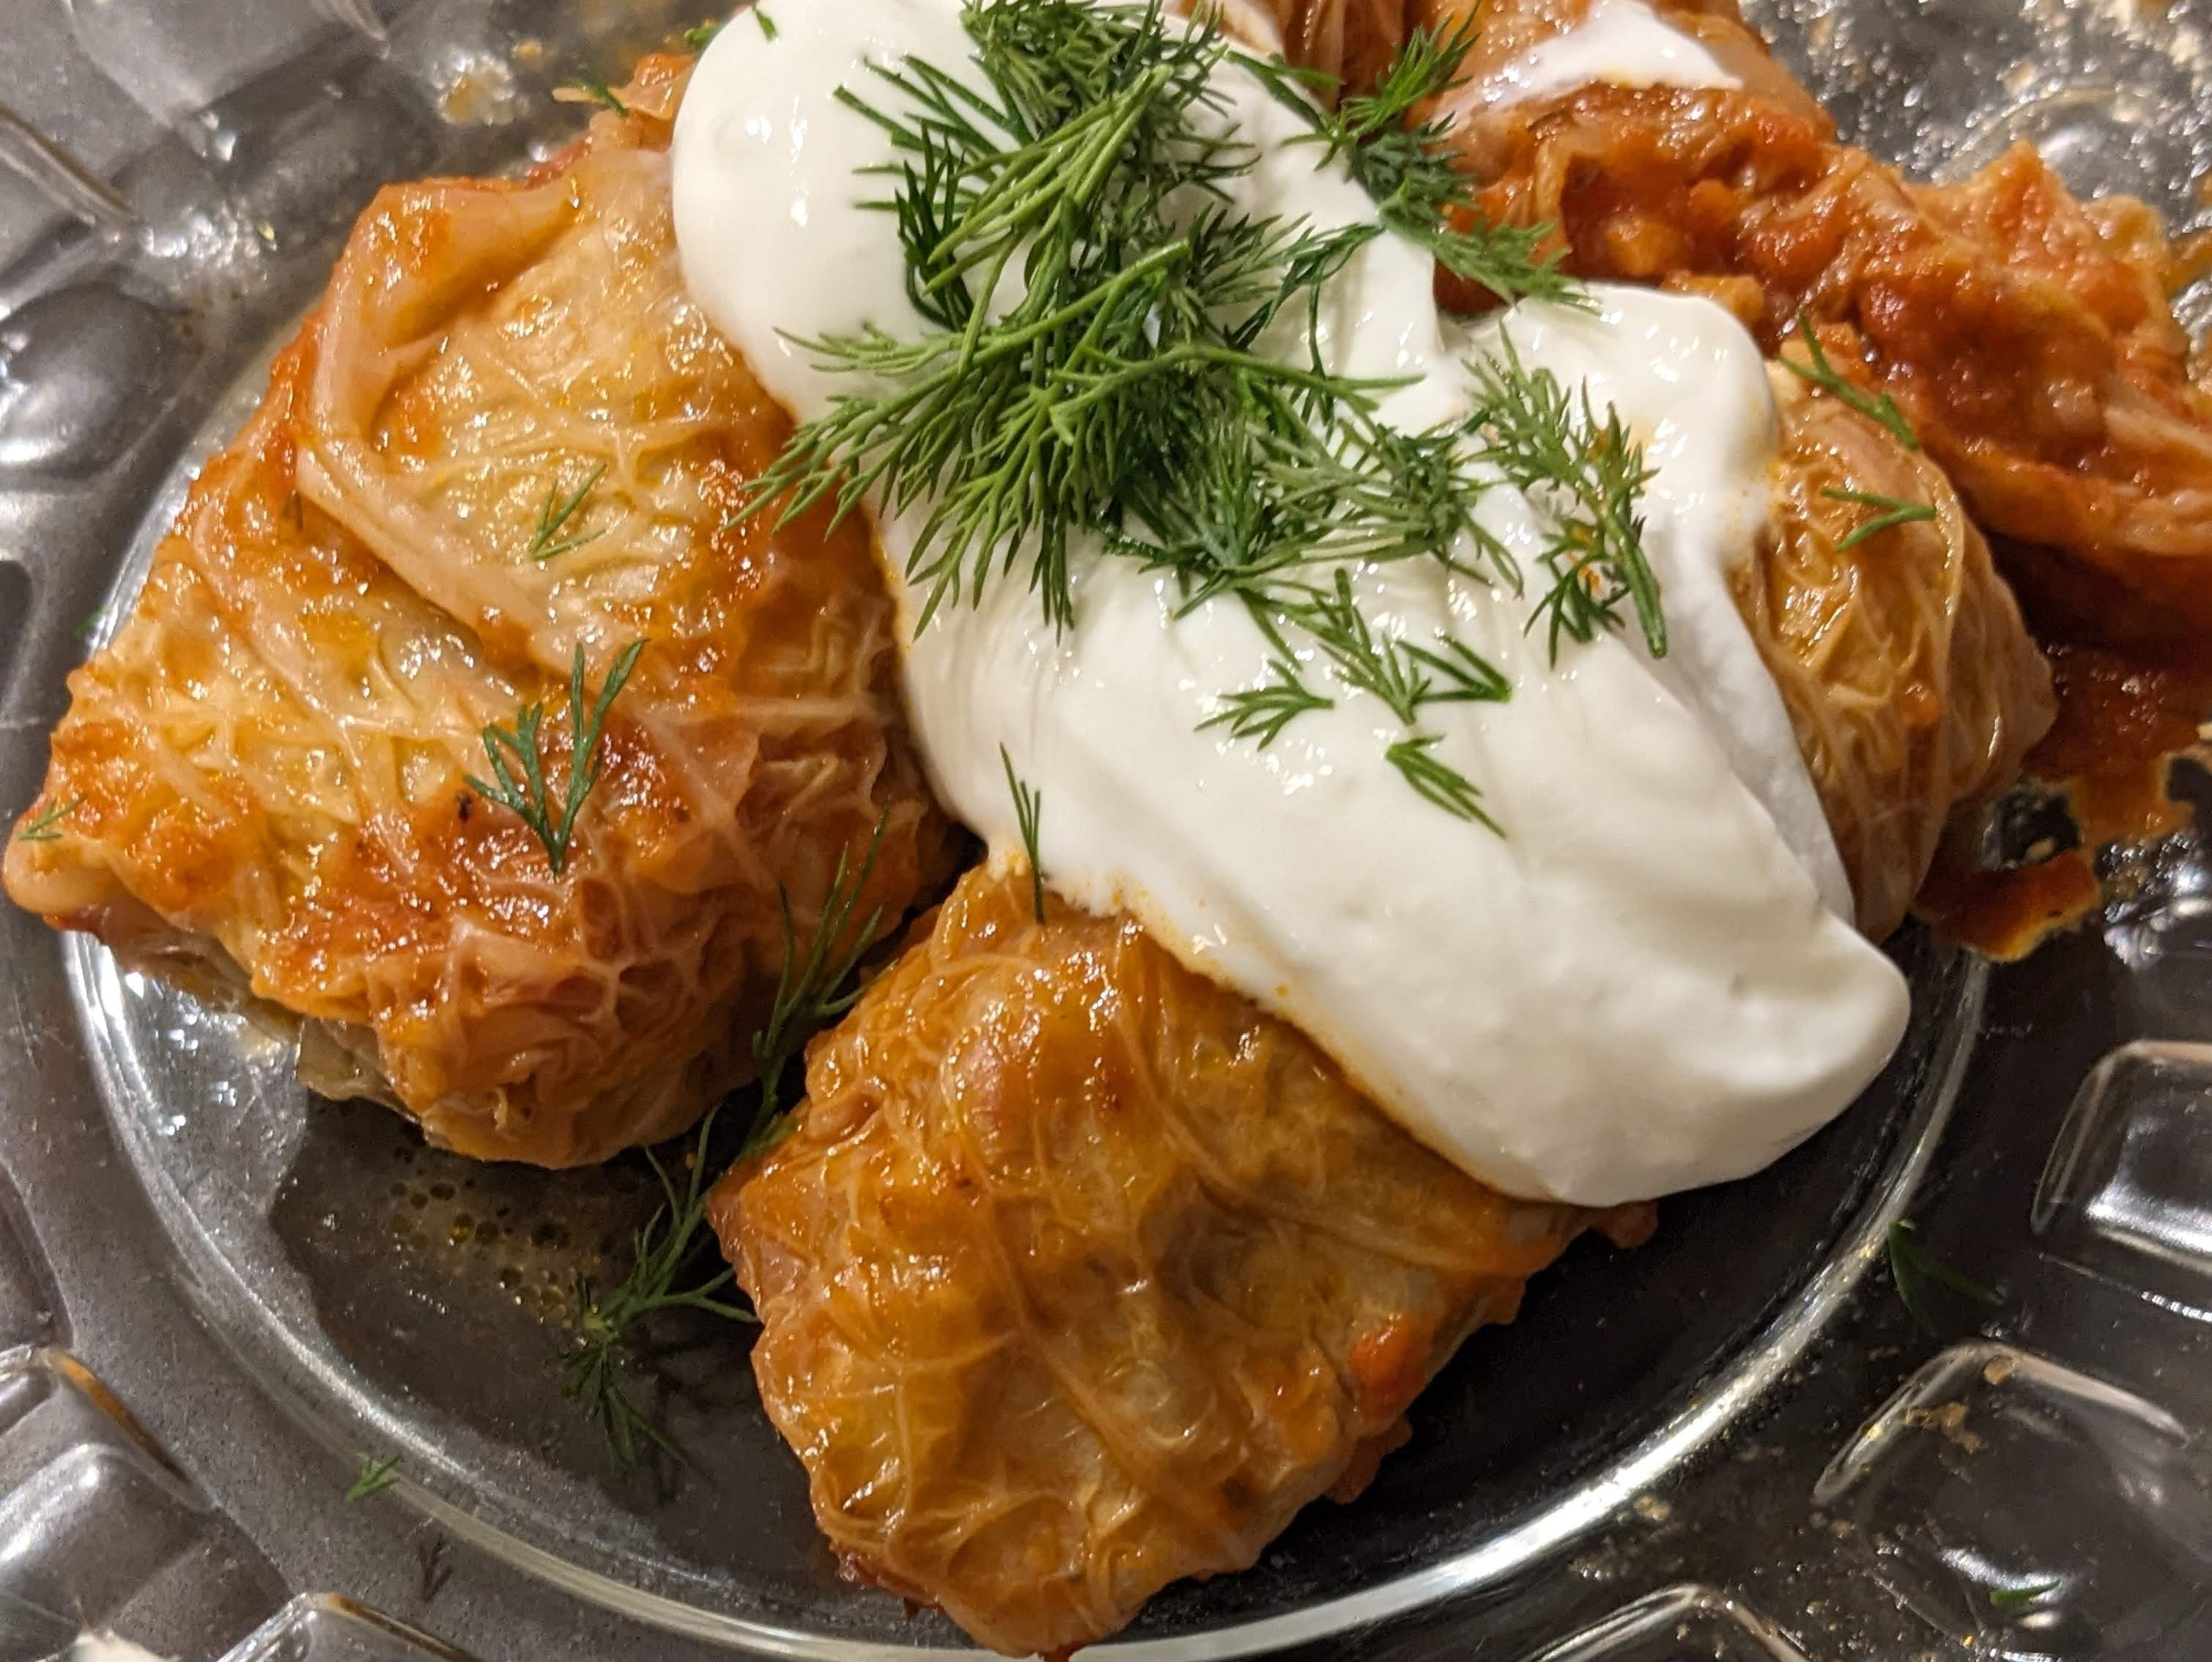
\includegraphics[width=60mm]{dermardiros/images/PXL_20240128_010747331.PORTRAIT.ORIGINAL.jpg}
  \caption{Topped with yogurt and dill!}
  \label{fig:fig}
\end{marginfigure}[20pt]

% \newthought{}
% \bigskip

\begin{enumerate}
    \item Heat water and salt in a small pot.
    \item Remove each cabbage leaf gently and cut out the stem (middle hard part).
    \item Put a the leaves 3 at a time into the boiling water and leave for 1 min until they are tender.
    \item Put each boiled leaf on a plate lined with paper towel. Reserved cabbage water.
    \item In a medium bowl, mix ground beef, rice, onion, salt and pepper.
    \item Place teared cabbage leaves at the bottom of a large wide pot. Roll dolma with meat filling and place each into the pot tightly together, seam-side down. Make 2 layers at most.
    \item Mix 1 cup of water to 3/4 cup Passata and add it to the pot containing the dolma.
    \item Place the pot on the stove, cover and heat on high. Reduce the heat once simmering and cook for 30-40min.
    \item Add more water/Passata if necessary to get the consistency you like, adjust seasoning.
    \item Serve with yogurt and dill/parsley.
\end{enumerate}

\marginnote{
    If have leftover meat mixture, can make kept balls or fill some tomatoes and place them next to the rolled dolma to cook together.
    Can be frozen after cooking/cooling.
    If using 1 whole savoy cabbage, double the filling quantities.
}
\chapter{Mantuh}
\label{ch:mantuh}
\index{meal}
\index{dumplings}
\index{meat}

\marginnote{
    \textbf{Makes 2~full pans} \\
    Prep time: 2-3~hours \\
    Cook time: 30~minutes \\
    \vspace*{\baselineskip}

    \textbf{Ingredients for dough} \\
    4~cups all-purpose flour \\
    ¼~cup milk \\
    ½~tsp salt \\
    1~cup lukewarm water + ¼ to ½~cup more (as much as dough takes) \\
    Oil (to work dough with hands) \\
    \vspace*{\baselineskip}

    \textbf{Ingredients for meat} \\
    1~medium onion, thinly chopped \\
    1~lb ground lean beef \\
    Salt \& pepper to taste \\
    Armenian or Lebanese pepper
}

\textit{Meat-filled dumplings}

Family member: Metzma Lucie

\begin{enumerate}
    \item Chop onion and cook in a medium pot for 1-2~minutes until soft.
    \item Add lean ground beef, salt, pepper and Armenian pepper.
    \item Cook until little or no water is left from the meat.

    % TODO: did we want to split this up into sections?
    \item In a large bowl, mix flour and salt.
    \item Mix in milk using a spoon. Add 1~cup water and mix with hands.
    \item Add a little oil to hands to help dough unstick.
    \item Add ¼ to ½~cup water slowly while mixing, until you get a soft dough.
    \item You can add up to 2~handfuls of oil.

    \item Flatten dough using a rolling pin or a pasta machine.
    \item Cut into 1.5-inch squares, fill with some meat and pinch sides.
    \item Place month on a baking sheet lined with parchment paper, leaving some space between each.
    \item Cook at 350\degree F for about 30~minutes, until evenly browned.
    \item Eat with yogurt, sriracha and sprinkle with sumac!
\end{enumerate}

After first cooking in oven, Sybil would normally cook them in a broth and eat as a soup. You can top with a little yogurt in there too!
Can store cooked in bags in the freezer, reheat in oven before eating.

\twosidecaptionfigure{dermardiros/images/Mantuh.jpg}{dermardiros/images/Mantuh 2.JPG}{(Left) Mantuh making for the Armenian bazar, 2018, (Right) Baked mantuh}{fig:mantuh2}

\chapter{Foul}
\label{ch:foul}
\index{dish}
\index{beans}

\marginnote{
    \textbf{Makes 1 bowl?} \\
    Prep time: 10 minutes \\
    Cook time: 20 minutes \\
    \vspace*{\baselineskip}

    1 can foul, brand? \\
    1 onion, diced \\
    ? Water \\
    ? Lemons, juiced \\
    Olive oil \\
    Cumin \\
    Parsley
}

\textit{Egyptian fava beans}

Family member: Sybil

\begin{enumerate}
    \item Empty the fava beans and bean liquid from the can into a medium pot.
    \item Add some water, the lemon juice and cook the foul until it thickens.
    \item Taste and adjust with cumin.
    \item To serve, top with chopped parsley, a drizzle of olive oil and the onions.
\end{enumerate}

Serve warm with tahini and fresh pita bread.

\chapter{Koubeba}
\label{ch:koubeba}
\index{meal}
\index{meat}

\marginnote{
    \textbf{Makes 1~round baking dish} \\
    Prep time: 45~minutes \\
    Cook time: 1~hour \\
    \vspace*{\baselineskip}
    
    \textbf{Ingredients for koubeba layers} \\
    2~cups bulgur, fin \#1 \\
    500~g ground beef, extra lean \\
    Salt \& pepper \\
    \vspace*{\baselineskip}
    
    \textbf{Ingredients for filling} \\
    500~g ground beef, extra lean \\
    1~onion, diced \\
    All spice \\
    Pine nuts \\
    Corinthian raisins \\
    Salt \& pepper \\
    Melted butter and oil 
}

\textit{Baked kibbeh}

Family member: Sybil

\begin{enumerate}
    \item In a bowl, add the bulgur, cover with hot water and set aside.
    \item Once soaked, use your hand to knead the soaked bulgur for a few minutes, until all is mashed together. Add it to a larger bowl with the ½~kg of ground meat, salt and pepper. Mix everything well and set aside.
    \item For the filling, cook the onion with some oil on a pan until soft. Add the other ½~kg of ground meat and cook until meat is browned. Add the spices, raisins and pine nuts. Cook the filling until evenly browned and let it cool.
    \item Grease a 12-inch round baking dish with olive oil.
    \item Using your hands, spread half of the koubeba mixture evenly on the bottom of the greased baking dish.
    \item Spoon all the filling on top of the bottom layer.
    \item Using the remaining koubeba mixture, spread it evenly on top of the filling and press it until no more middle layer shows. Use water as needed to create a smooth top layer.
    \item Using a large Knife, slice the Koubeba diagonally to form diamond-shaped slices. Poke holes with a souvlaki stick and pour a mixture of melted butter and oil in the holes. You can top with pine nuts over each slice if you want to be fancy and drizzle with a little olive oil.
    \item Bake at 350\degree F for about 45~minutes, until top is browned.
    \item Once cool, eat with yogurt!
\end{enumerate}

\chapter{Souloukefteh}
\label{ch:souloukefteh}
\index{meal}
\index{meat}
\index{soup}
\textit{Soupe boulettes de viande}

Family member: Metzma Lucie

\marginnote[20pt]{\\
    \textbf{Makes 4 servings} \\
    Prep time: \\
    Cook time: 3 1/2-4 hours \\
    \vspace*{\baselineskip}
    
    \textbf{Ingredients for stock} \\
    1 beef shank or 2 veal shanks (about 1 lb) \\
    1 large yellow onion \\ 
    2 bay leaves \\
    8-10 cups of water \\
    1 tsp tomato paste \\
    \vspace*{\baselineskip}

    \textbf{Ingredients for soup} \\
    Reserved stock \\ 
    1 lb ground beef \\
    1/2 large yellow onion \\
    1/4 cup rice, Calrose \\
    1/2 cup parsley, chopped \\
    1 egg \\
    Salt \& pepper to taste
    3 white or Russet potatoes, cubed \\
    Carrots, chopped (optional) \\
    1/4 cup rice, Calrose (or orzo) \\
}

\begin{enumerate}
    \item Add all the ingredients for the stock except the tomato paste in a large pot and bring it to a boil. Cook for 2.5 hours.
    \item Remove the shank, take off the meat and add it to the stock. Remove the onion dd the tomato paste and mix.
    \item In a bowl, grate the onion and mix it with the meat, rice, parsley and egg. Add salt and pepper and let stand for about 15 minutes.
    \item Form 1.5-inch balls of the meat mixture while bringing the stock to a boil.
    \item Add the meatballs and reserved 1/4 cup rice (or orzo). Reduce to a simmer.
    \item After 15 minutes, add the potatoes (and carrots if using) and continue cooking for 30 minutes to 1 hour.
\end{enumerate}

\chapter{Bâtons Salés}
\label{ch:batonsale}
\index{dessert}
\index{cookie}

\marginnote{
    \textbf{Makes 40-60~cookies} \\
    Prep time: 45~minutes \\
    Cook time: 30~minutes \\
    \vspace*{\baselineskip}

    5~cups all-purpose flour \\
    3~tsp baking powder \\
    1~tsp salt \\
    1~cup warm water \\
    1 1/2~cups vegetable oil \\
    1/2~cup zaatar \\
    1~egg \\
    Nigella seeds
}

\textit{Savoury sticks}

Family member: Nene Hermine

\begin{enumerate}
    \item In a large bowl, mix all the ingredients except the egg and nigella seeds. Add an additional flour if needed to obtain a non-sticky soft yet pliable dough.
    \item Shape into 4-5~inch thin ropes. Fold each rope in half then form a twisted rope.
    \item Place on baking sheet lined with parchment.
    \item Lightly brush with egg wash and sprinkle with nigella seeds.
    \item Bake at 350\degree F for about 30~minutes.
\end{enumerate}

Sybil's trick: You can freeze 2/3~of the cookies once they have baked and cooled.

\chapter{Beureg}
\label{ch:beureg}
\index{meal}
\index{spinach}
\index{feta}

\marginnote{
    \textbf{Makes 1~large pan} \\
    Prep time: 1~hour \\
    Cook time: 1~hour \\
    \vspace*{\baselineskip}

    \textbf{Ingredients for dough} \\
    3~cups all-purpose flour \\
    ¾~cup vegetable oil, Canola \\
    ¼~cup butter, melted \\
    1~tsp baking powder \\
    1~egg \\
    1~cup milk, room temperature \\
    \vspace*{\baselineskip}

    \textbf{Ingredients for filling} \\
    1~onion, diced \\
    142~g fresh spinach or 1~packet frozen, thawed \\
    250~g feta, grated \\
    2-3~eggs \\
    Milk \\
    \vspace*{\baselineskip}

    \textbf{Egg wash} \\
    1~egg \\
    Nigella or sesame seeds
}

\textit{Spinach and cheese pie}

Family member: Sybil

\begin{enumerate}
    \item In a large bowl, mix all the ingredients for the dough together until a dough forms. Cover the bowl with plastic wrap and keep aside.
    \item To make the filling, cook the onion with a some oil in a pan.
    \item Add the fresh or thawed spinach, and cook on medium heat.
    \item Pour the mix into a bowl. Once cool, add the grated feta, the eggs and a little bit of milk. Mix well using a fork.
    \item Divide the dough in 2~parts, and roll them out using a rolling pin. Use some flour if needed on the working surface.
    \item In a rectangular dish, place one half. Spread the filling on top. Cover with the second dough.
    \item For egg wash, whisk 1~egg yolk with a little bit of water in a bowl. Brush the egg wash onto the top and sprinkle with nigella or sesame seeds.
    \item Bake at 350\degree F on the top rack for about 1~hour.
\end{enumerate}


\chapter{Quiche}
\label{ch:hamquiche}
\index{meat}
\index{meal}
\index{pie}
\index{brunch}

\marginnote{
    \textbf{Makes 1 quiche} \\
    Prep time: 30-45 minutes \\
    Cook time: 45 minutes \\
    \vspace*{\baselineskip}

    Half the pie dough \\
    320 grams of shredded cheese, Italian 4 cheese \\
    6 slices of ham, cut \\
    5 eggs \\
    1 cup (250 ml) 15\% cooking cream \\
    Pepper 
}

Family member: Sybil

\begin{enumerate}
    \item Prepare a 9 inch pie plate with the pie dough.
    \item In a bowl, mix the cream and eggs with a whisk. Add the cut ham and shredded cheese.
    \item Preheat oven to 350\degree F.
    \item Pour the mix on the pie crust and top with ground pepper.
    \item Bake for 1 hour at 350\degree F.
\end{enumerate}

\marginnote{
    You can replace half of the 15\% cooking cream with milk.
}

\chapter{Ham Quiche}
\label{ch:hamquiche}
\index{meat}
\index{meal}
\index{pie}
\index{brunch}

\marginnote{
    \textbf{Makes 1~quiche} \\
    Prep time: 30-45~minutes \\
    Cook time: 45~minutes \\
    \vspace*{\baselineskip}

    Pastry for one 9-inch piecrust, well chilled, Tenderflake Deep Dish pie crust \\
    Margarine \\
    1~large onion, chopped, about 1~cup \\
    1~tablespoon all purpose flour \\
    120~g/¼~lb of Gruyere cheese \\
    120~g/¼~lb of Swiss cheese \\
    1~slice of smoked ham \\
    3~large eggs \\
    1~cup half-and-half cream
}

Family member: Aunt Joanne

\begin{enumerate}
    \item Prepare a 9-inch piecrust, or take out the Tenderflake Deep Dish pie crust.
    \item In a small skillet over medium heat, melt 2~tablespoons of margarine. Cook the chopped union until tender, about 5~minutes, stirring occasionally. Once cooked, spread it evenly in the pie crust.
    \item Preheat oven to 400\degree F.
    \item Chop the smoked ham slice into little cubes.
    \item Shred both Gruyere and Swiss cheese. In medium bowl, toss the cheeses with flour.
    \item Mix in the cubed ham with the cheeses and spread them over the onion in the piecrust.
    \item Beat 3~eggs with 1~cup of half-and-half cream. Pour it over the shredded cheese and ham mix in piecrust.
    \item Bake for 10~minutes. Reduce the oven to 325\degree F and bake for 30~to 35~minutes longer until knife inserted in center comes out clean.
    \item Let the pie stand 10~minutes, then cut into wedges.
\end{enumerate}

\chapter{Meat Pies}
\label{ch:meatpies}
\index{meat}
\index{meal}
\index{pie}
\index{brunch}

\marginnote{
    \textbf{Makes 6~meat pies} \\
    Prep time: 3~hours \\
    Cook time: 45~minutes, or 20~minutes for partially cooked (frozen) pies \vspace*{\baselineskip}

    5~pounds minced veal (2.3~kg) \\
    4~pounds minced pork (1.8~kg) \\
    2~pounds minced lean beef (907~g or 1~kg) \\
    Small pack of bacon with maple \\
    Becel margarine \\
    1/4~onion chopped in small pieces \\
    5~tsp Provence spices \\
    Black pepper \\
    3~cups of red or white wine \\
    1 1/2~cups of Italian bread crumbs (up to 3~cups if needed) \\
    2~packages of pie dough from Metro (Francois Hubert pie dough 1~kg makes 5~bases) \\
    Flour \\
    2~eggs
}

Family member: Aunt Joanne

\begin{enumerate}
    \item Place the bacon on parchment paper on a tray and cook it in the oven. Once cooked, place it in bowl.
    \item Put margarine in a frying pan and cook the onion until soft; remove it and put it in bowl.
    \item Put margarine in a frying pan and cook the minced meats, sprinkling the Provence spice and pepper as they cook.
    \item When all is cooked, mix the 3~meats, onion and bacon, and split into 2~big casseroles to further cook on stove top. Add the wine, split into both casseroles. Cook for 20~minutes on low heat, stirring occasionally.
    \item Add the breadcrumbs, split into both casseroles containing the meat mixture.
    \item Let stand 10~minutes. If enough liquid is absorbed by the breadcrumbs, no need to add any more. If not, add more breadcrumbs until excess liquid is absorbed. Set aside to cool.
    \item Preheat the oven to 500\degree F.
    \item On a floured work surface, roll out the pie dough and cut it in 6~sections. Line 8-9~inch pie pans with the first circle of pie dough and divide the meat filling into all 6~pans. Roll out remaining pie dough into circles and place a second circle of pie dough over each pie, covering the meat mixture.
    \item Cut some steam vents in the centre of the crust. Seal the edges together with fork, then cut off excess.
    \item In a bowl, beat the eggs and brush the crust with the egg wash. Transfer the pies to the oven.
    \item Reduce temperature to 400\degree F and bake until the meat pies are golden brown, about 45~minutes.
    \item For frozen pies, partially bake them; only bake for 20~minutes and let them cool. Place an aluminum paper on top of each pie and then put them in a large freezer bag. Freeze. To reheat frozen pies, bake about 30~minutes, checking when the crust is golden.
\end{enumerate}

\chapter{Pasta and Meat Sauce}
\label{ch:pastameatsauce}
\index{meat}
\index{meal}
\index{pasta}

\marginnote{
    \textbf{Makes 6-8 portions} \\
    Prep time: 30-45 minutes \\
    Cook time: 5 hours \\
    \vspace*{\baselineskip}

    2 tbsp olive oil \\
    1 finely chopped small onion \\
    1 garlic clove, crushed (optional) \\
    1/2 pound of minced veal \\
    1/2 pound of minced pork \\
    1/2 pound of minced beef \\
    300 g Chianti Red Wine Rosette de Lyon dried sausage by Papille \\
    1 can (796ml) Aylmer Diced Tomatoes with Italian Spices \\
    2 cans (156ml) of Unico Tomato Paste \\
    1 1/4 cups of red wine \\
    2 tsp dried oregano \\
    Fresh basil \\
    1 tsp sugar \\
    Salt \\
    Pepper \\
    Pasta of your choice
}

Family member: Aunt Joanne

\begin{enumerate}
    \item Slice the dried sausage and put it aside.
    \item Heat the olive oil in a skillet and gently cook the onion and garlic, stirring for 10 minutes until softened.
    \item Add the minced veal, pork and beef and cook until they change colour, stirring constantly and breaking up the meat. Stir in the dried sausage.
    \item Purée the diced tomatoes in a blender and pour into a cooking pot. You can also leave them diced as is.
    \item Mix each can of tomato paste in a cup of water and add them to the cooking pot.
    \item Add 1-1/4 cups of red wine. Add sugar, salt and pepper.
    \item Stir in the meat/onion/garlic mixture into the pot.
    \item Add dried oregano and fresh shredded basil and bring to a boil while stirring.
    \item Cover and lower the heat to a gentle simmer for 3 to 4 hours, stirring occasionally.
\end{enumerate}

AJ usually prepares a larger quantity in a very big pot and freezes the sauce in many containers.

\chapter{Biscuits Grand-Mère}
\label{ch:biscuits_grandmere}
\index{dessert}
\index{mahleb}
\index{sesame}
\index{cookies}

\marginnote{
    \textbf{Makes 40-60 cookies} \\
    Prep time: 45 minutes \\
    Cook time: 20 minutes \\
    \vspace*{\baselineskip}

    4 cups all-purpose flour, Robin Hood \\
    2 tsp baking powder \\
    1/2 tsp mahleb, ground \\
    3/4 cup sugar \\
    1/2 cup vegetable oil, Canola \\
    1/2 cup margarine, Becel \\
    1 cup milk \\
    Egg yolks \\
    Sesame seeds
}

\marginalfigure{dermardiros/images/Biscuits metzma.jpg}{Biscuits Grand-Mère}{fig:biscuits_grandmere}

\textit{Circle sesame cookies}

Family member: Metzma Lucie

\begin{enumerate}
    \item In a large bowl, mix the flour, baking powder, mahleb and sugar.
    \item Add the oil and margarine. Add the milk accordingly.
    \item Shape into thin ropes, then into 2-inch circles.
    \item Place on baking sheet lined with parchment.
    \item For egg wash, whisk egg yolks with a little bit of water in a bowl. Brush the egg wash onto cookies and sprinkle with sesame seeds.
    \item Bake at 350\degree F on the top rack for about 20 minutes, rotate pan once after 10 minutes.
\end{enumerate}

\twosidecaptionfigure{dermardiros/images/Family.jpg}{dermardiros/images/Family_boys.jpg}{Metzma's birthday, 2024}{fig:biscuits_grandmere2}
\chapter{Grandma Cake / Gateau à Sybil}
\label{ch:grandma_cake}
\index{dessert}
\index{chocolate}
\index{cake}

\marginnote{
    \textbf{Makes 1 bundt cake} \\
    Prep time: 20 minutes \\
    Cook time: 45 minutes - 1 hour \\
    \vspace*{\baselineskip}

    2 cups sugar \\
    3-4 eggs \\
    1 tsp vanilla extract \\
    3 cups all-purpose flour \\
    3 tsp baking powder \\
    1 cup milk \\
    1 cup vegetable oil \\
    \vspace*{\baselineskip}

    2 tsp cocoa powder
}

\textit{Marble bundt cake}

Family member: Metzma Lucie \& Sybil

\begin{enumerate}
    \item In a large bowl, whisk the sugar, eggs and vanilla.
    \item In another bowl, whisk the flour and baking powder. Add the dry ingredients to the sugar/egg mixture above in 2 times.
    \item Add the milk, then once completely incorporated, add the oil.
    \item Place half of the mix in a separate bowl, and sift in the cocoa powder. Mix it well.
    \item Grease a loaf pan and line with parchment.
    \item Pour the chocolate mix in the pan, then the vanilla. Use a knife to swirl both mixes.
    \item Bake at 350\degree F for 45 minutes to 1 hour.
\end{enumerate}

\twosidecaptionfigure{dermardiros/images/Grandma cake 1.JPG}{dermardiros/images/Grandma cake 2.jpg}{Marble cake with various designs}{fig:grandmacake}

Sybil's alternatives: orange zest and 1 cup chocolate chips, 2 bananas, 1 cup raisins. You can use more cocoa powder if you want to have a deeper chocolate taste.

\chapter{Chocolate Pudding Cake}
\label{ch:chocolatefridgecake}
\index{dessert}
\index{chocolate}
\index{cake}
\index{cookies}

\marginnote{
    \textbf{Makes 1~cake} \\
    Prep time: 20~minutes + chill overnight in the fridge\\
    Cook time: 5~minutes \\
    \vspace*{\baselineskip}

     1~pack of Sheriff chocolate pudding \\
     1~pack of tea biscuits, Dare Traditions Social Tea brand
}

\textit{Chocolate fridge cake with cookies}

Family member: Metzma Lucie \& Dan

\newthought{Vasken} would eat half a pan of this.
\bigskip

\begin{enumerate}
    \item Follow the instructions on the chocolate pudding box.
    \item In a Pyrex or other baking dish, place tea biscuits to make a layer. You may need to break some cookies to cover all the bottom.
    \item While the pudding mixture is still hot, pour a thin layer on top of the cookies.
    \item Repeat layering cookies and pudding until desired height and finish with a layer of pudding at the very top.
    \item Refrigerate overnight.
\end{enumerate}

\twosidecaptionfigure{dermardiros/images/Grandma fridge cake 1.jpg}{dermardiros/images/Grandma fridge cake 2.jpg}{Chocolate cake made by Dan enjoyed with a coffee!}{fig:grandmacake}


\chapter{Khorabiè}
\label{ch:khorabie}
\index{dessert}
\index{cookies}
\index{dates}

\marginnote{
    \textbf{Makes 24+ cookies} \\
    Prep time: 2-3 hours \\
    Cook time: 12-15 minutes \\
    \vspace*{\baselineskip}

    1 cup vegetable oil \\
    1 cup milk \\
    250ml butter, melted (or unsalted margarine) \\
    1/2 packet of Crisco, melted \\
    3 tsp baking powder \\
    1 cup icing sugar \\
    6-6 1/2 cups flour \\
    1 kg dates, in puree (in a packet) \\
    Zest and juice of 1 orange 
}

\textit{Biscuits aux dattes}

Family member: Metzma Lucie


\marginalfigure{dermardiros/images/PXL_20240427_185332023.PORTRAIT.ORIGINAL.jpg}{Khorabiè mold}{fig:khorabie}

% \begin{figure}
%   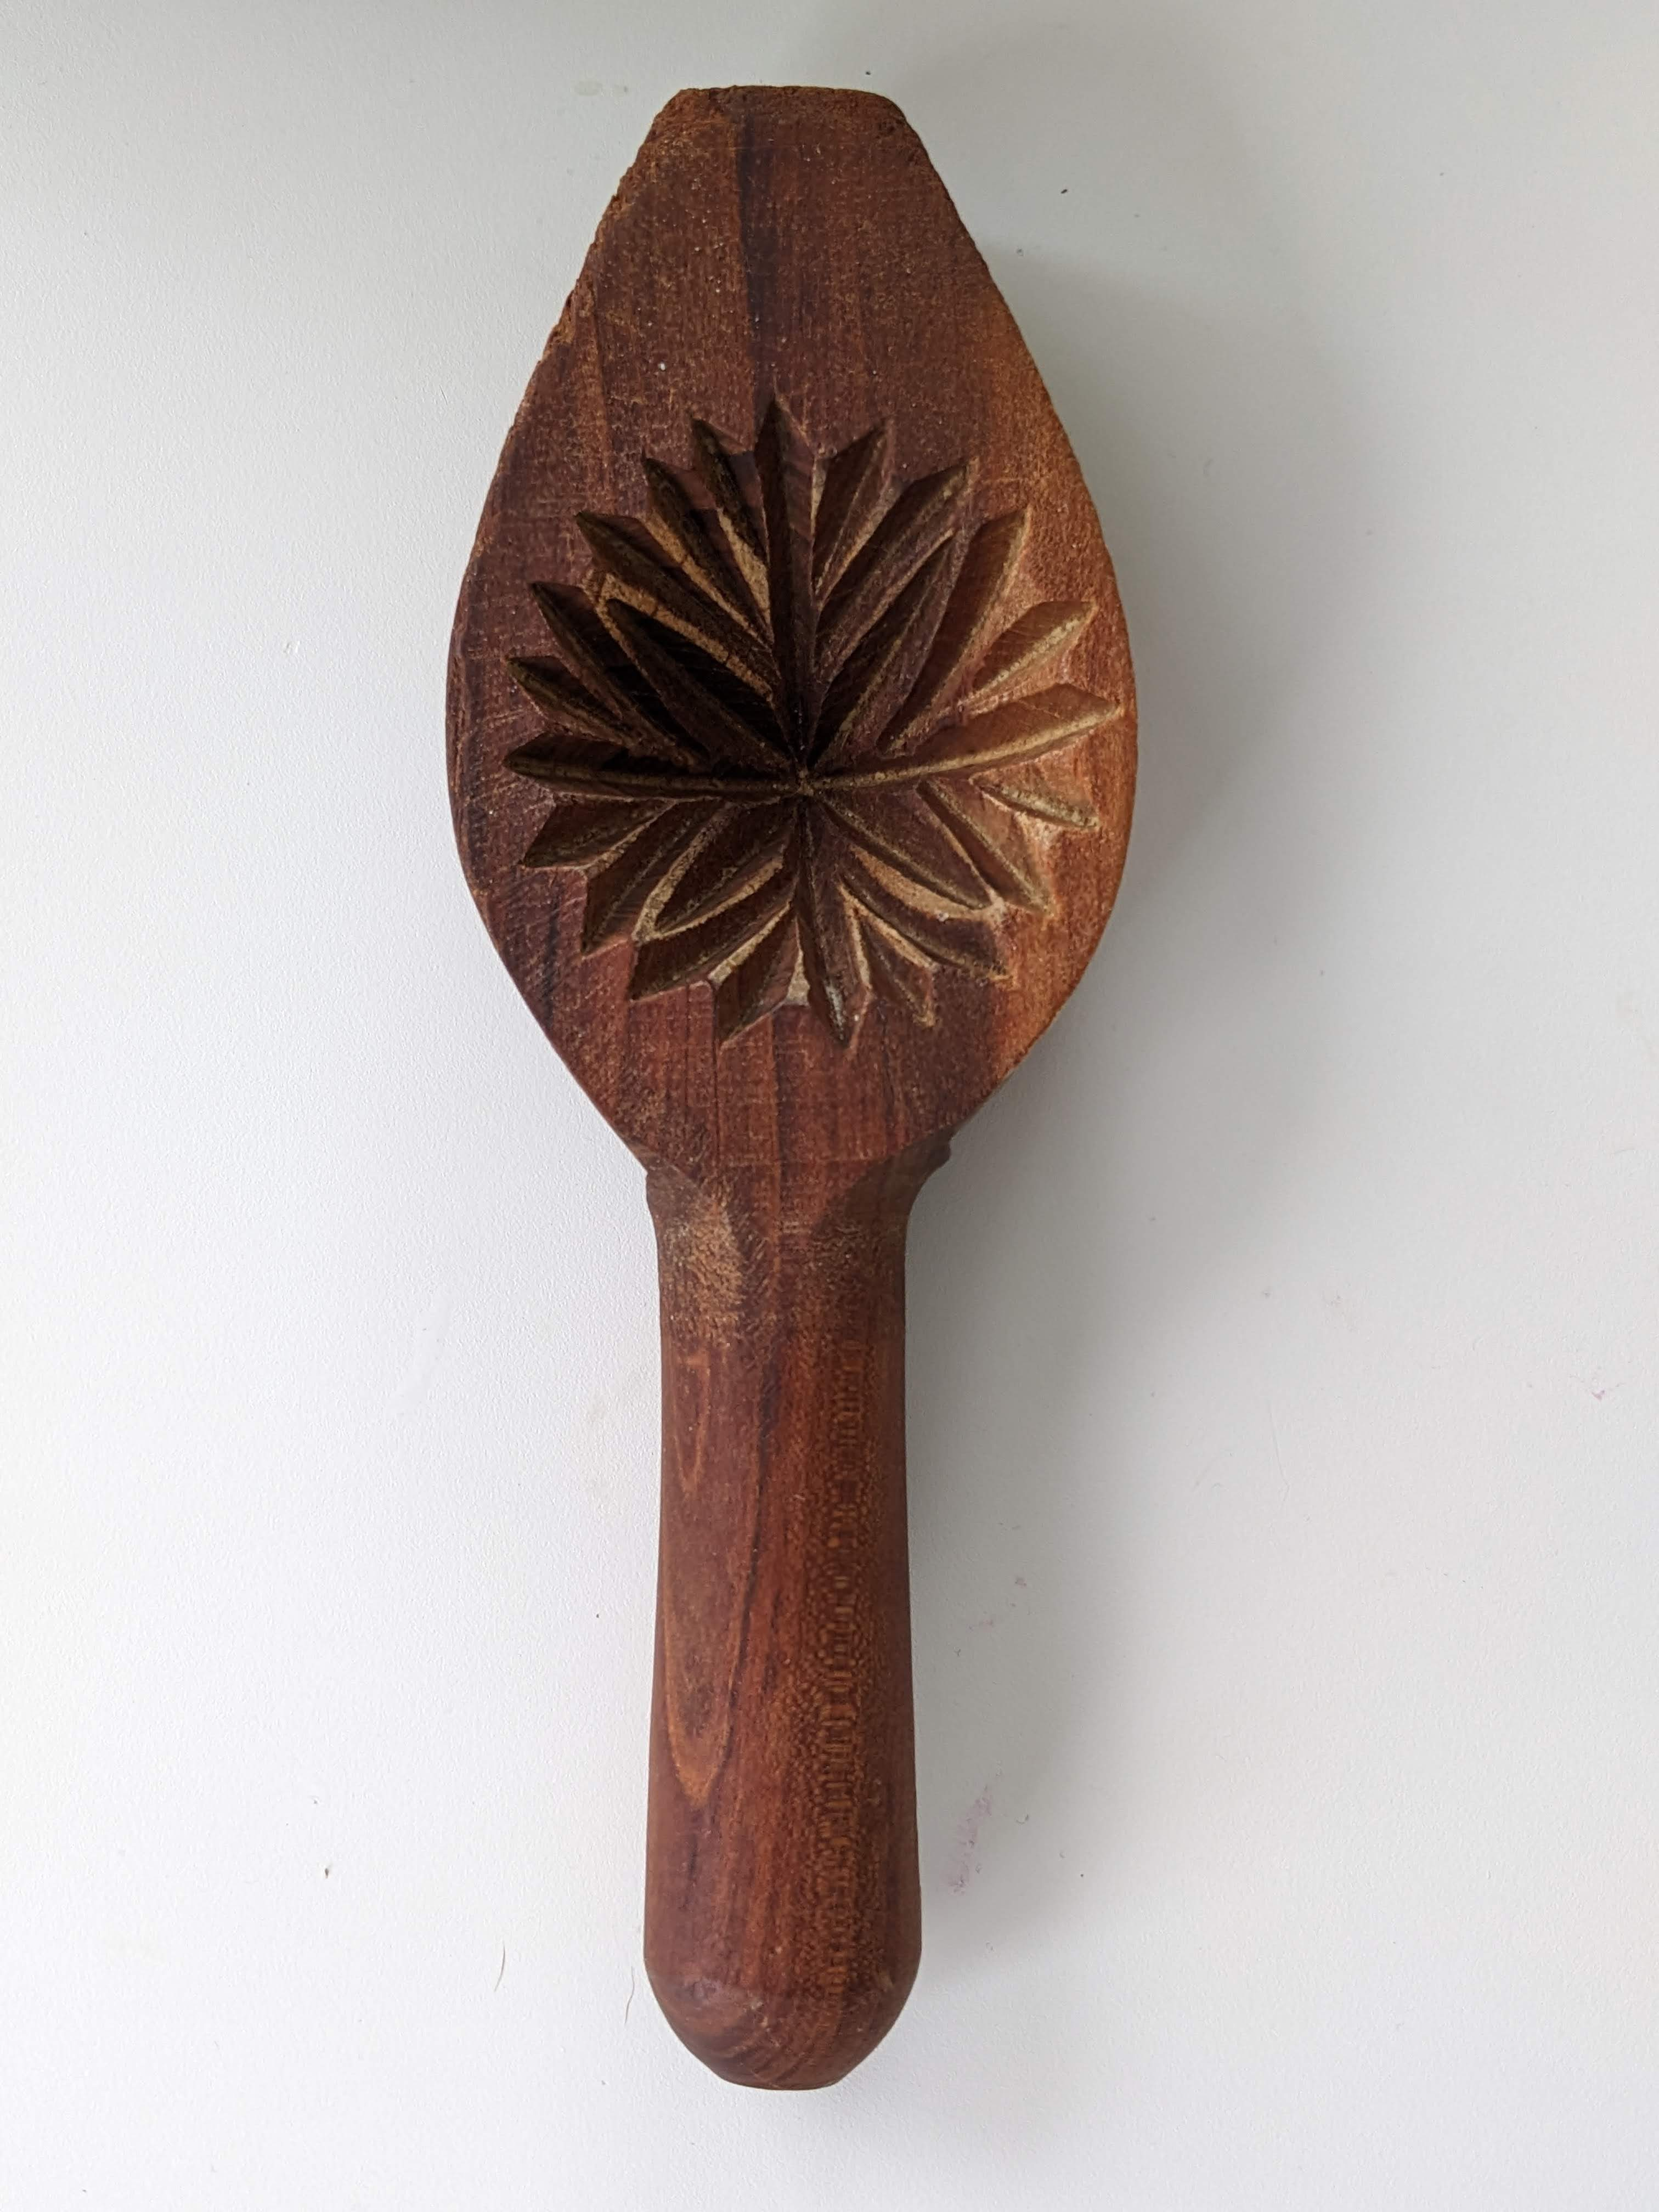
\includegraphics[width=60mm]{dermardiros/images/PXL_20240427_185332023.PORTRAIT.ORIGINAL.jpg}
%   \caption{Khorabiè mold}
% \end{figure}

\begin{enumerate}
    \item In a bowl, mix the oil, milk, melted butter and melted Crisco.
    \item In another bowl, mix the baking powder, icing sugar and flour.
    \item Sift the dry ingredients onto the wet ingredients, then mix with hands until you form a dough. You can add more flour as needed to form a ball.
    \item In a small bowl, mix the dates with the orange zest and orange juice.
    \item Shape balls of dough, make a small well in the center and stuff with the date filling. Enclose the dates in the center with the dough. 
    \item Lightly flour the wooden khorabie mold and gently press the ball inside the mold to obtain a shape on one side.
    \item Place the shaped cookies onto a baking sheet and bake 12-15 minutes on the middle rack at 350\degree F until the tops have a golden color. 
    \item Let cool and sift some icing sugar on top. Enjoy with coffee or tea!
\end{enumerate}

\chapter{Cheureg}
\label{ch:cheureg}
\index{dessert}
\index{bread}
\index{Easter}

\marginnote{
    \textbf{Makes 4-6 braids} \\
    Prep time: 5-6 hours \\
    Cook time: 30 minutes \\
    \vspace*{\baselineskip}

    6 eggs \\
    2 packets of traditional yeast \\
    2 tsp sugar \\
    1/2 tsp water \\
    10 cups all-purpose flour + 1/2 cup, Robin Hood \\
    Mahleb, ground \\
    2 cups of milk, lukewarm \\
    2 cups sugar \\
    1.5 cups of butter, melted \\
    Egg yolks, beaten for egg wash 
}

\textit{Easter bread}

Family member: Great Grandma

\begin{enumerate}
    \item In a large bowl, mix the flour, baking powder, mahleb and sugar.
    \item Add the oil and margarine. Add the milk accordingly.
    \item Shape into thin ropes, then into 2-inch circles.
    \item Place on baking sheet lined with parchment.
    \item In a small bowl, start yeast: place packets of yeast, 2 tsp sugar and water. Let for 15 minutes.
    \item In a large bowl, whisk the flour and mahlep. 
    \item Create a well in the dry ingredients and add the yeast mixture. Incorporate the flour into the yeast slowly.
    \item In a small bowl, beat the eggs slightly. Add them to the flour/yeast mixture above.
    \item In another bowl, add the sugar to the lukewarm milk and mix it. Add it to the flour/yeast/egg mixture and mix well.
    \item Slowly add the melted butter while mixing. Knead the dough until smooth.
    \item Cover the dough, and let proof for 3-4 hours in a bowl covered with plastic wrap.
    \item Punch down the dough, shape into braids. Cover with a clean towel and let rise for 1 hour. Brush the braids with egg wash.
    \item Bake at 350\degree F for about 30 minutes, sprinkle with sugar when cooled.
    If large, thick braids - on bottom rack.
    If small braids - on top rack.
\end{enumerate}

\chapter{Anoushabour}
\label{ch:anoushabour}
\index{dessert}
\index{pudding}

\marginnote{
    \textbf{Makes 1 bowl} \\
    Prep time: 30 minutes + overnight rest \\
    Cook time: 45 minutes \\
    \vspace*{\baselineskip}

    1 cup pearl barley \\
    1/4 cup sugar \\
    Yellow and sultan raisins \\
    Dried apricots, quartered \\
    1/4 tsp rose water or orange blossom water, optional
}

\marginalfigure{dermardiros/images/Anoushabour.JPG}{Anoushabour from New Year's Eve brunch at AJ and Eddy's in 2011!}{fig:anoushabour}

\textit{Sweet barley pudding}

Family member: Sybil

\begin{enumerate}
    \item In a pot, cook pearl barley in 2 cups of water for 10 minutes.
    \item Remove from stove, let cool. Cover and leave overnight.
    \item The next day, the barley should be plump. Add a little more water, the raisins and apricots. Continue to cook for a few minutes. There should be water in the pot (not completely absorbed).
    \item After 15 minutes, add the sugar and continue cooking for 15 minutes more.
    \item Once done, remove from heat, add rose water or orange blossom water if using, and let it cool.
    \item Pour in a large glass bowl and serve.
\end{enumerate}

\chapter{Katnabour}
\label{ch:katnabour}
\index{dessert}
\index{rice}
\index{pudding}

\marginnote{
    \textbf{Makes 1 bowl} \\
    Prep time: 5 minutes \\
    Cook time: 30 minutes \\
    \vspace*{\baselineskip}

    1/2 cup rice, Calrose \\
    3 cups milk, 2\% \\
    3 tbsp sugar 
}

\textit{Rice pudding}

Family member: Sybil

\newthought{Secret tip:} microwave for a few second and serve warm in a small coffee cup with a sprinkle of cinnamon.

% \begin{figure}
%   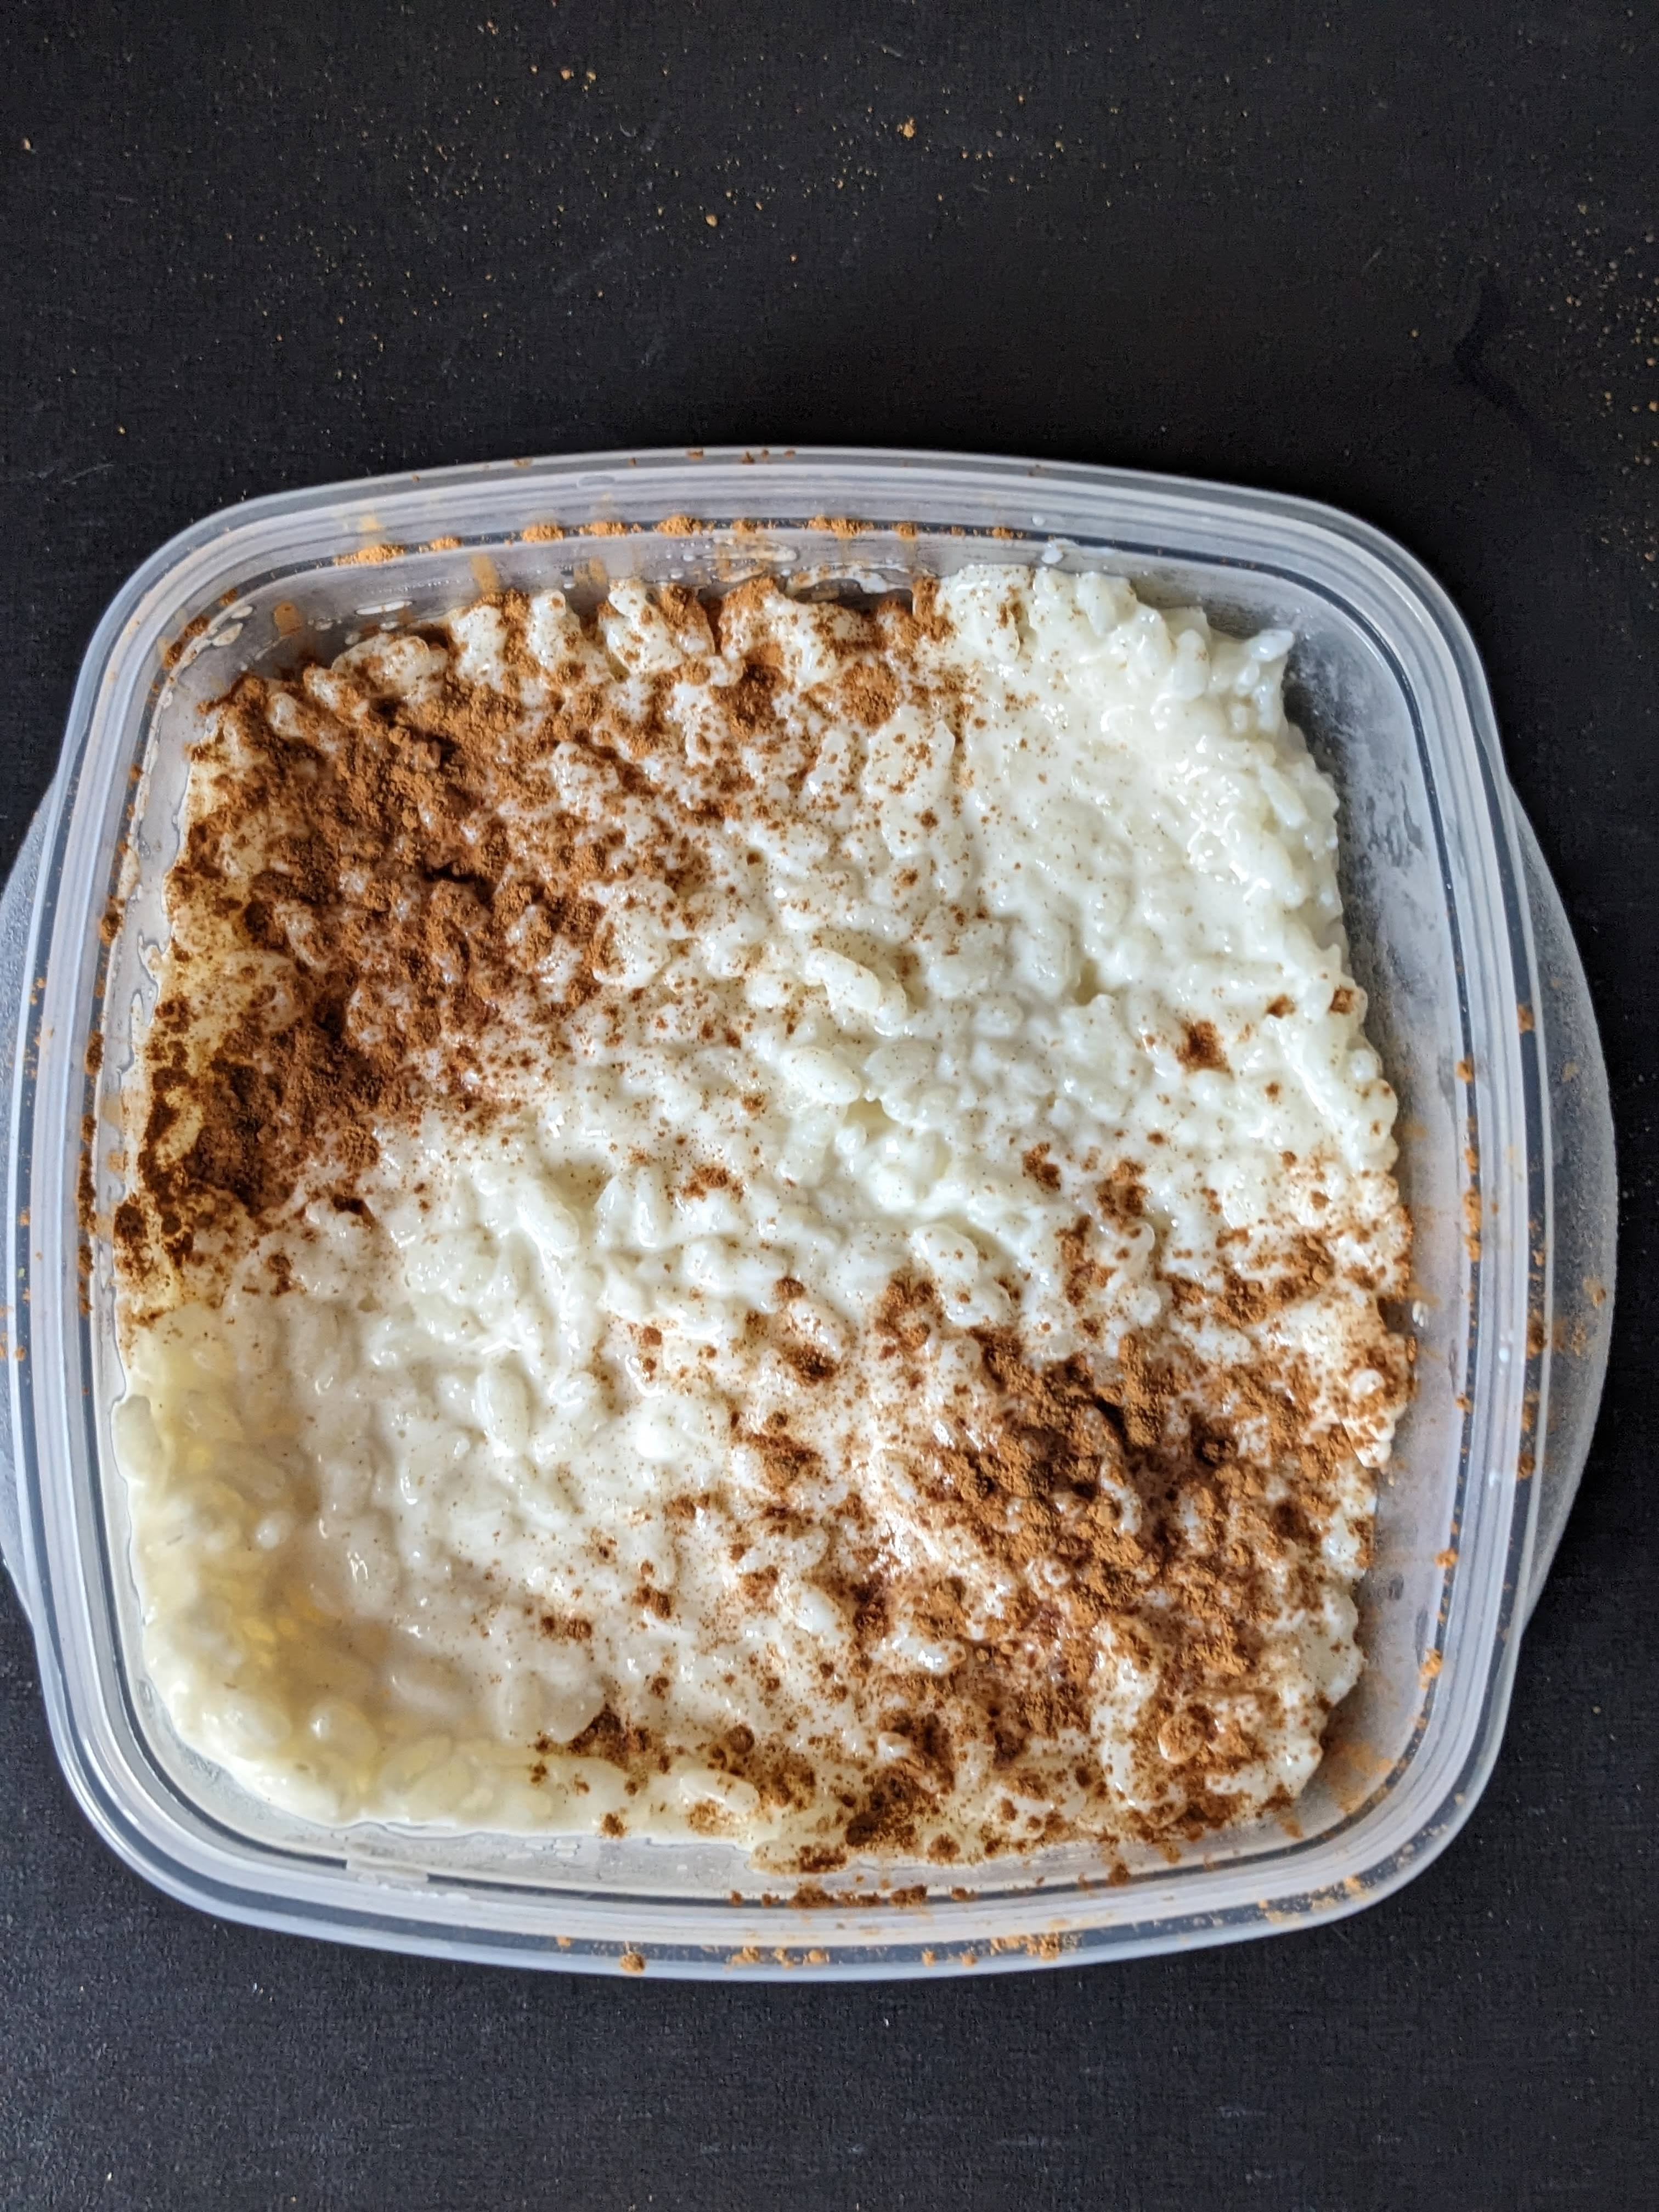
\includegraphics[width=60mm]{dermardiros/images/Rice pudding.jpg}
%   \caption{Anoushabour made in Barcelona}
% \end{figure}

\marginalfigure{dermardiros/images/Rice pudding.jpg}{Anoushabour made in Barcelona}{fig:katnabour}

\begin{enumerate}
    \item In a pot, cook the rice in 1 cup of milk on low heat.
    \item Gradually add 1 cup of milk at a time, once milk has been absorbed.
    \item When all the milk has been added and the rice is cooked, add the sugar. 
    \item Cook on low heat for maximum 5 minutes then set the pot aside to cool.
\end{enumerate}

\chapter{Christmas Yule Log}
\label{ch:yulelog}
\index{dessert}
\index{chocolate}
\index{cake}
\index{Christmas}

Family member: Aunt Joanne

\marginnote[20pt]{\\
    \textbf{Makes 1 yule log} \\
    Prep time: 2-3 hours + setting time in the fridge \\
    Cook time: 15-20 minutes \\
    \vspace*{\baselineskip}

\textbf{Ingredients for the cake:} \\
    5 eggs, separated at room temperature \\
    1 cup confectioners’ sugar \\
    1/8 tsp salt \\
    2 1/2 cups whipping cream \\
    3/4 cup cocoa powder \\
    \vspace*{\baselineskip}

\textbf{Ingredients for the Mocha-Cream Filling:} \\
    3 cups whipping cream \\
    1 cup cocoa powder \\
    1/2 cup confectioners’ sugar \\
    3-4 tbsp Kahlua \\
    \vspace*{\baselineskip}

    \textbf{For decoration (optional):} \\
    Lindt chocolate balls (dark, milk, white) \\
    Raspberries \\
    Chocolate Santa Clause or Snowman \\
}

% \newthought
% \bigskip

\begin{enumerate}
    \item Preheat oven to 400\degree F. Grease the bottom of pan with margarine. Place parchment paper on top, and spray Pam on the parchment paper.
    \item In a large bowl with the mixer at high speed, beat egg whites until soft peaks form. Beating at high speed, gradually sprinkle in 1/2 cup confectioners’ sugar, beating thoroughly after each addition. Continue beating until the egg whites stand in stiff, glossy peaks. Set aside.
    \item In small bowl with same beaters and with the mixer at high speed, beat egg yolks until thick and lemon-colored. Reduce speed to low; beat in the salt, 1/2 cup confectioners’ sugar and 3 tbsp cocoa powder, occasionally scraping bowl with rubber spatula.
    \item Using the wire whisk or rubber spatula, gently fold the yolk mixture into the beaten whites just until the mixture is blended. Spread the batter evenly in the pan and bake 15 minutes or until top springs back when lightly touched with finger.
    \item Prepare a clean cloth towel by sprinkling it with cocoa powder.
    \item When the cake is done, with small spatula, immediately loosen its edges from the side of pan; invert the cake onto the prepared towel. Gently peel the parchment paper from bottom of cake. Roll the towel with the cake from narrow end, jelly-roll fashion. Let it cool completely, placing it seam side down on wire rack.
    \item Meanwhile, prepare the Mocha-Cream Filling. In a large bowl with the mixer at medium speed, beat the whipping cream, cocoa powder, confectioners’ sugar and Kahlua until stiff peaks form.
    \item When the cake is cool, unroll it from the towel and evenly spread the Mocha-Cream Filling on the cake.
    \item Starting at the narrow end, roll up the cake, without the towel this time. Place the cake, seam side down on a platter. Evenly spread the filling on the rolled up cake.
    \item If desired, you can cut a piece at the end of the log cake and place it on the top of the cake – far left side to resemble a knot in the log. Spread the filling on the slice too.
\end{enumerate}

\marginnote{
    You can decorate the top of the log cake either with:
    \vspace*{\baselineskip}
    - Lindt chocolate balls, alternating white, dark, milk chocolate. You can put raspberries between the chocolate balls \\
    - Chocolate Santa Clause or Snowman \\
}

\begin{figure}
  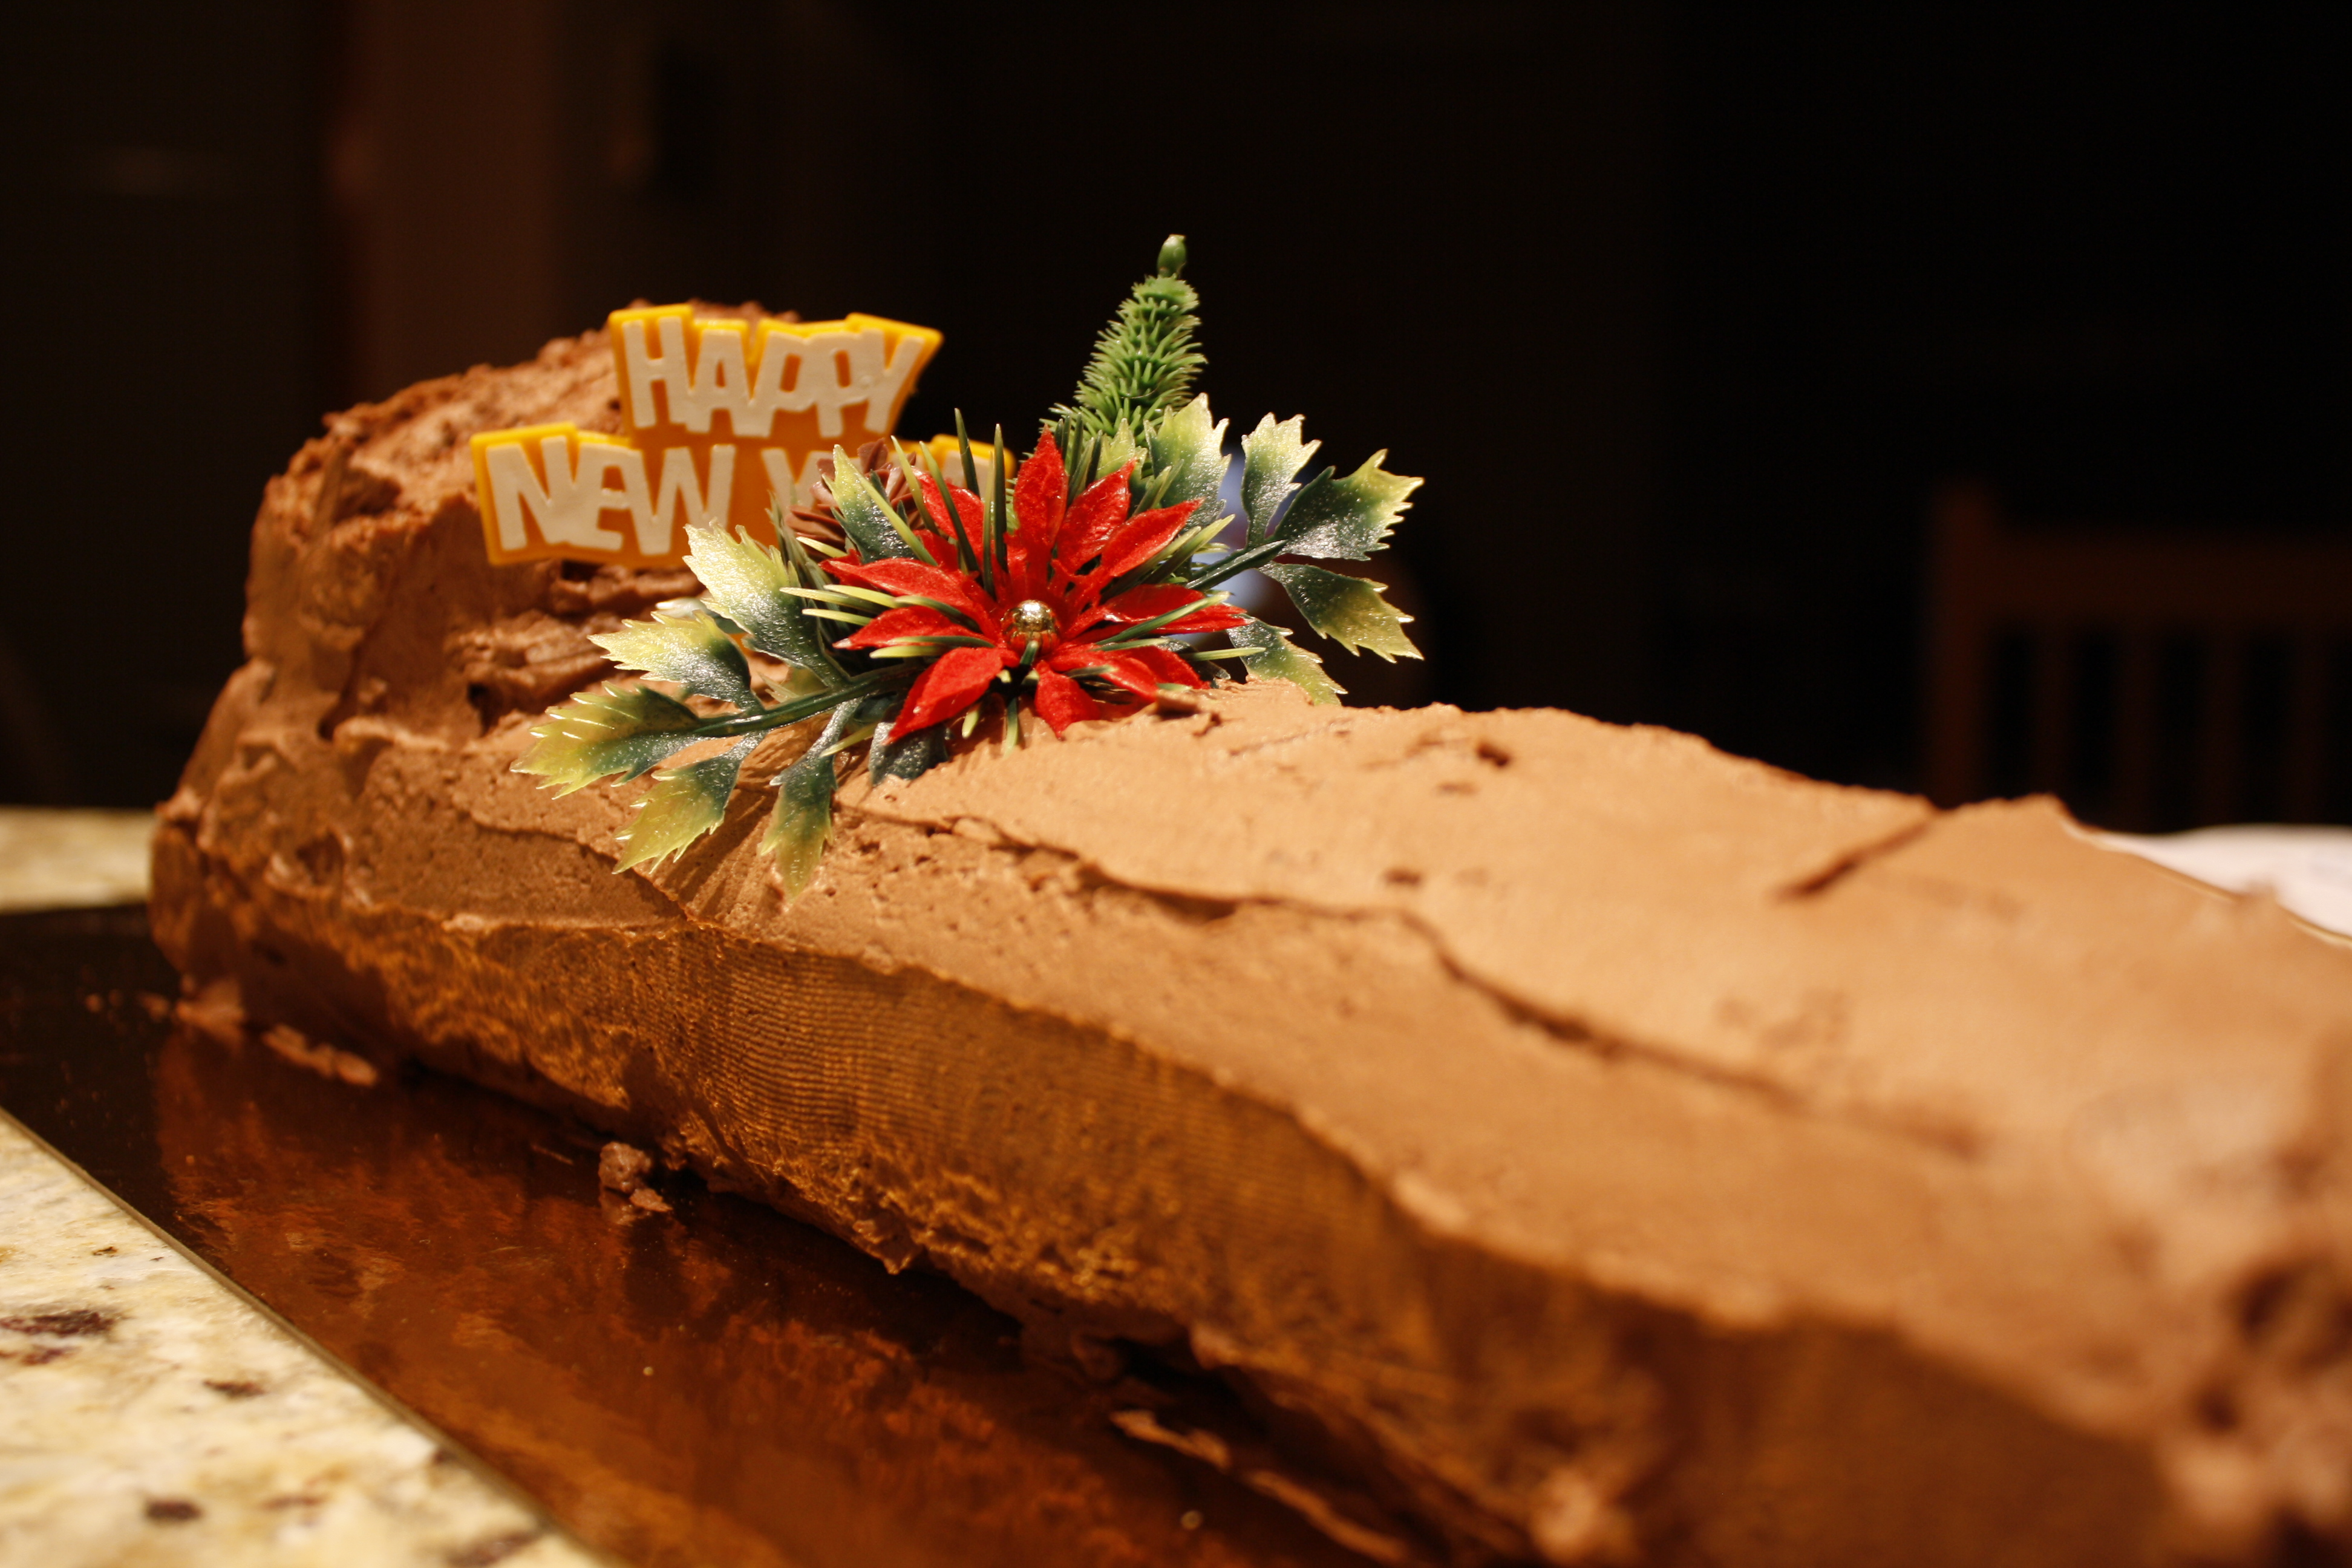
\includegraphics[width=60mm]{dermardiros/images/Logcake.JPG}
    \caption{Yule Log we made with AJ in 2011}
  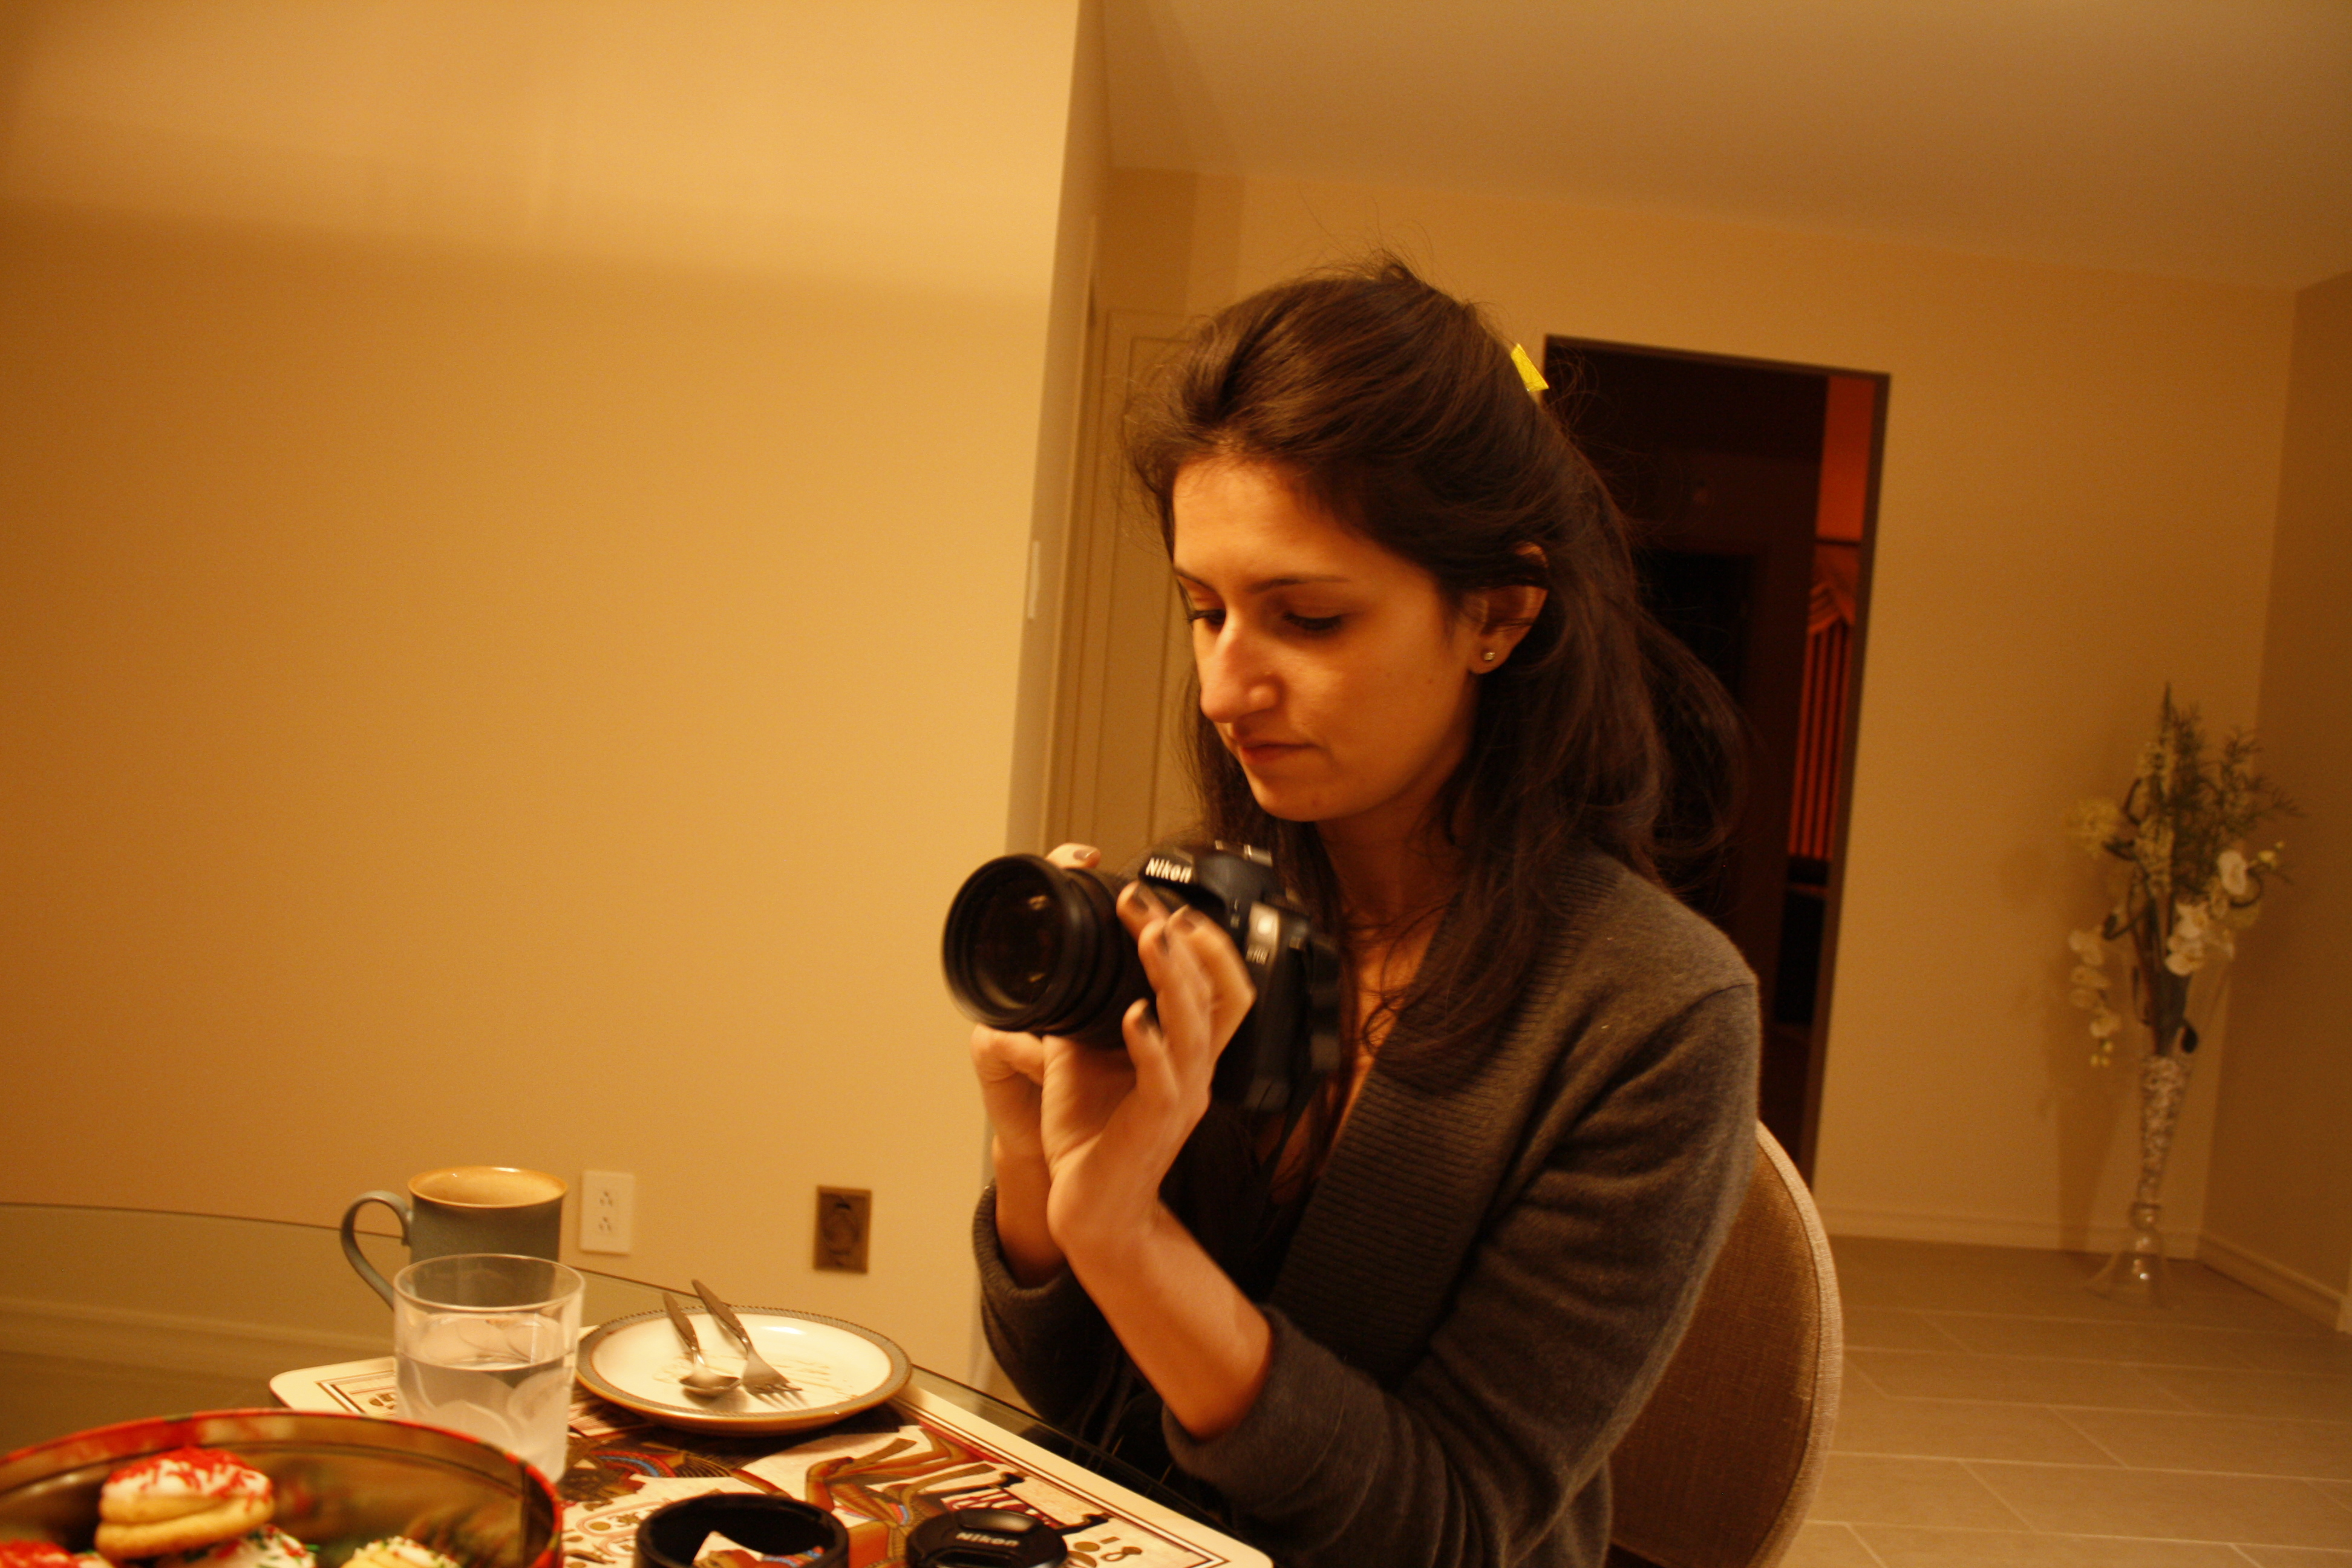
\includegraphics[width=60mm]{dermardiros/images/Logcake 3.JPG}    
\end{figure}
\chapter{Ciambalone}
\label{ch:ciambalone}
\index{dessert}
\index{Christmas}
\index{cake}

\marginnote{
    \textbf{Makes 1 bundt cake} \\
    Prep time: ? minutes \\
    Cook time: 35 minutes \\
    \vspace*{\baselineskip}

    125 ml (½ cup) margarine or butter, room temperature \\
    3 eggs \\
    175 ml (3/4 cups) sugar \\
    50 ml (1/4 cup) oil \\
    5 ml (1 tsp) vanilla extract \\
    175 ml (3/4 cups) milk (keep a little to put on top of batter before sprinkling with sugar) \\
    625 ml (2 ½ cups) all purpose flour \\
    15 ml (3 tsp) baking powder \\
    175 ml (3/4 cups) raisins (can substitute with Hershey’s caramel Chipits) \\
    175 ml (3/4 cups) Hershey’s mini chocolate chips \\
    2 red cherries \\
    2 green cherries 
}

\textit{Italian Bundt Cake}

Family member: Aunt Joanne

\begin{enumerate}
    \item Preheat oven at 180\degree C (350\degree F).
    \item Mix the sugar, butter or margarine, eggs and oil.
    \item Sift the flour and baking powder, and add them to egg mixture alternating with the milk.
    \item Add the vanilla extract and mix.
    \item Add the raisins and chocolate chips and mix with a spoon.
    \item Spray baking Pam on the bundt cake mold and pour the batter in the mold.
    \item Spread the leftover milk on top of the batter.
    \item Cut the cherries in half and place on top of batter (optional). Sprinkle a bit of sugar on top of batter.
    \item Bake for 35 minutes at 180\degree C (350\degree F). Let the cake cool in the mold and remove from mold after 30 minutes.
\end{enumerate}

% \begin{figure}
%   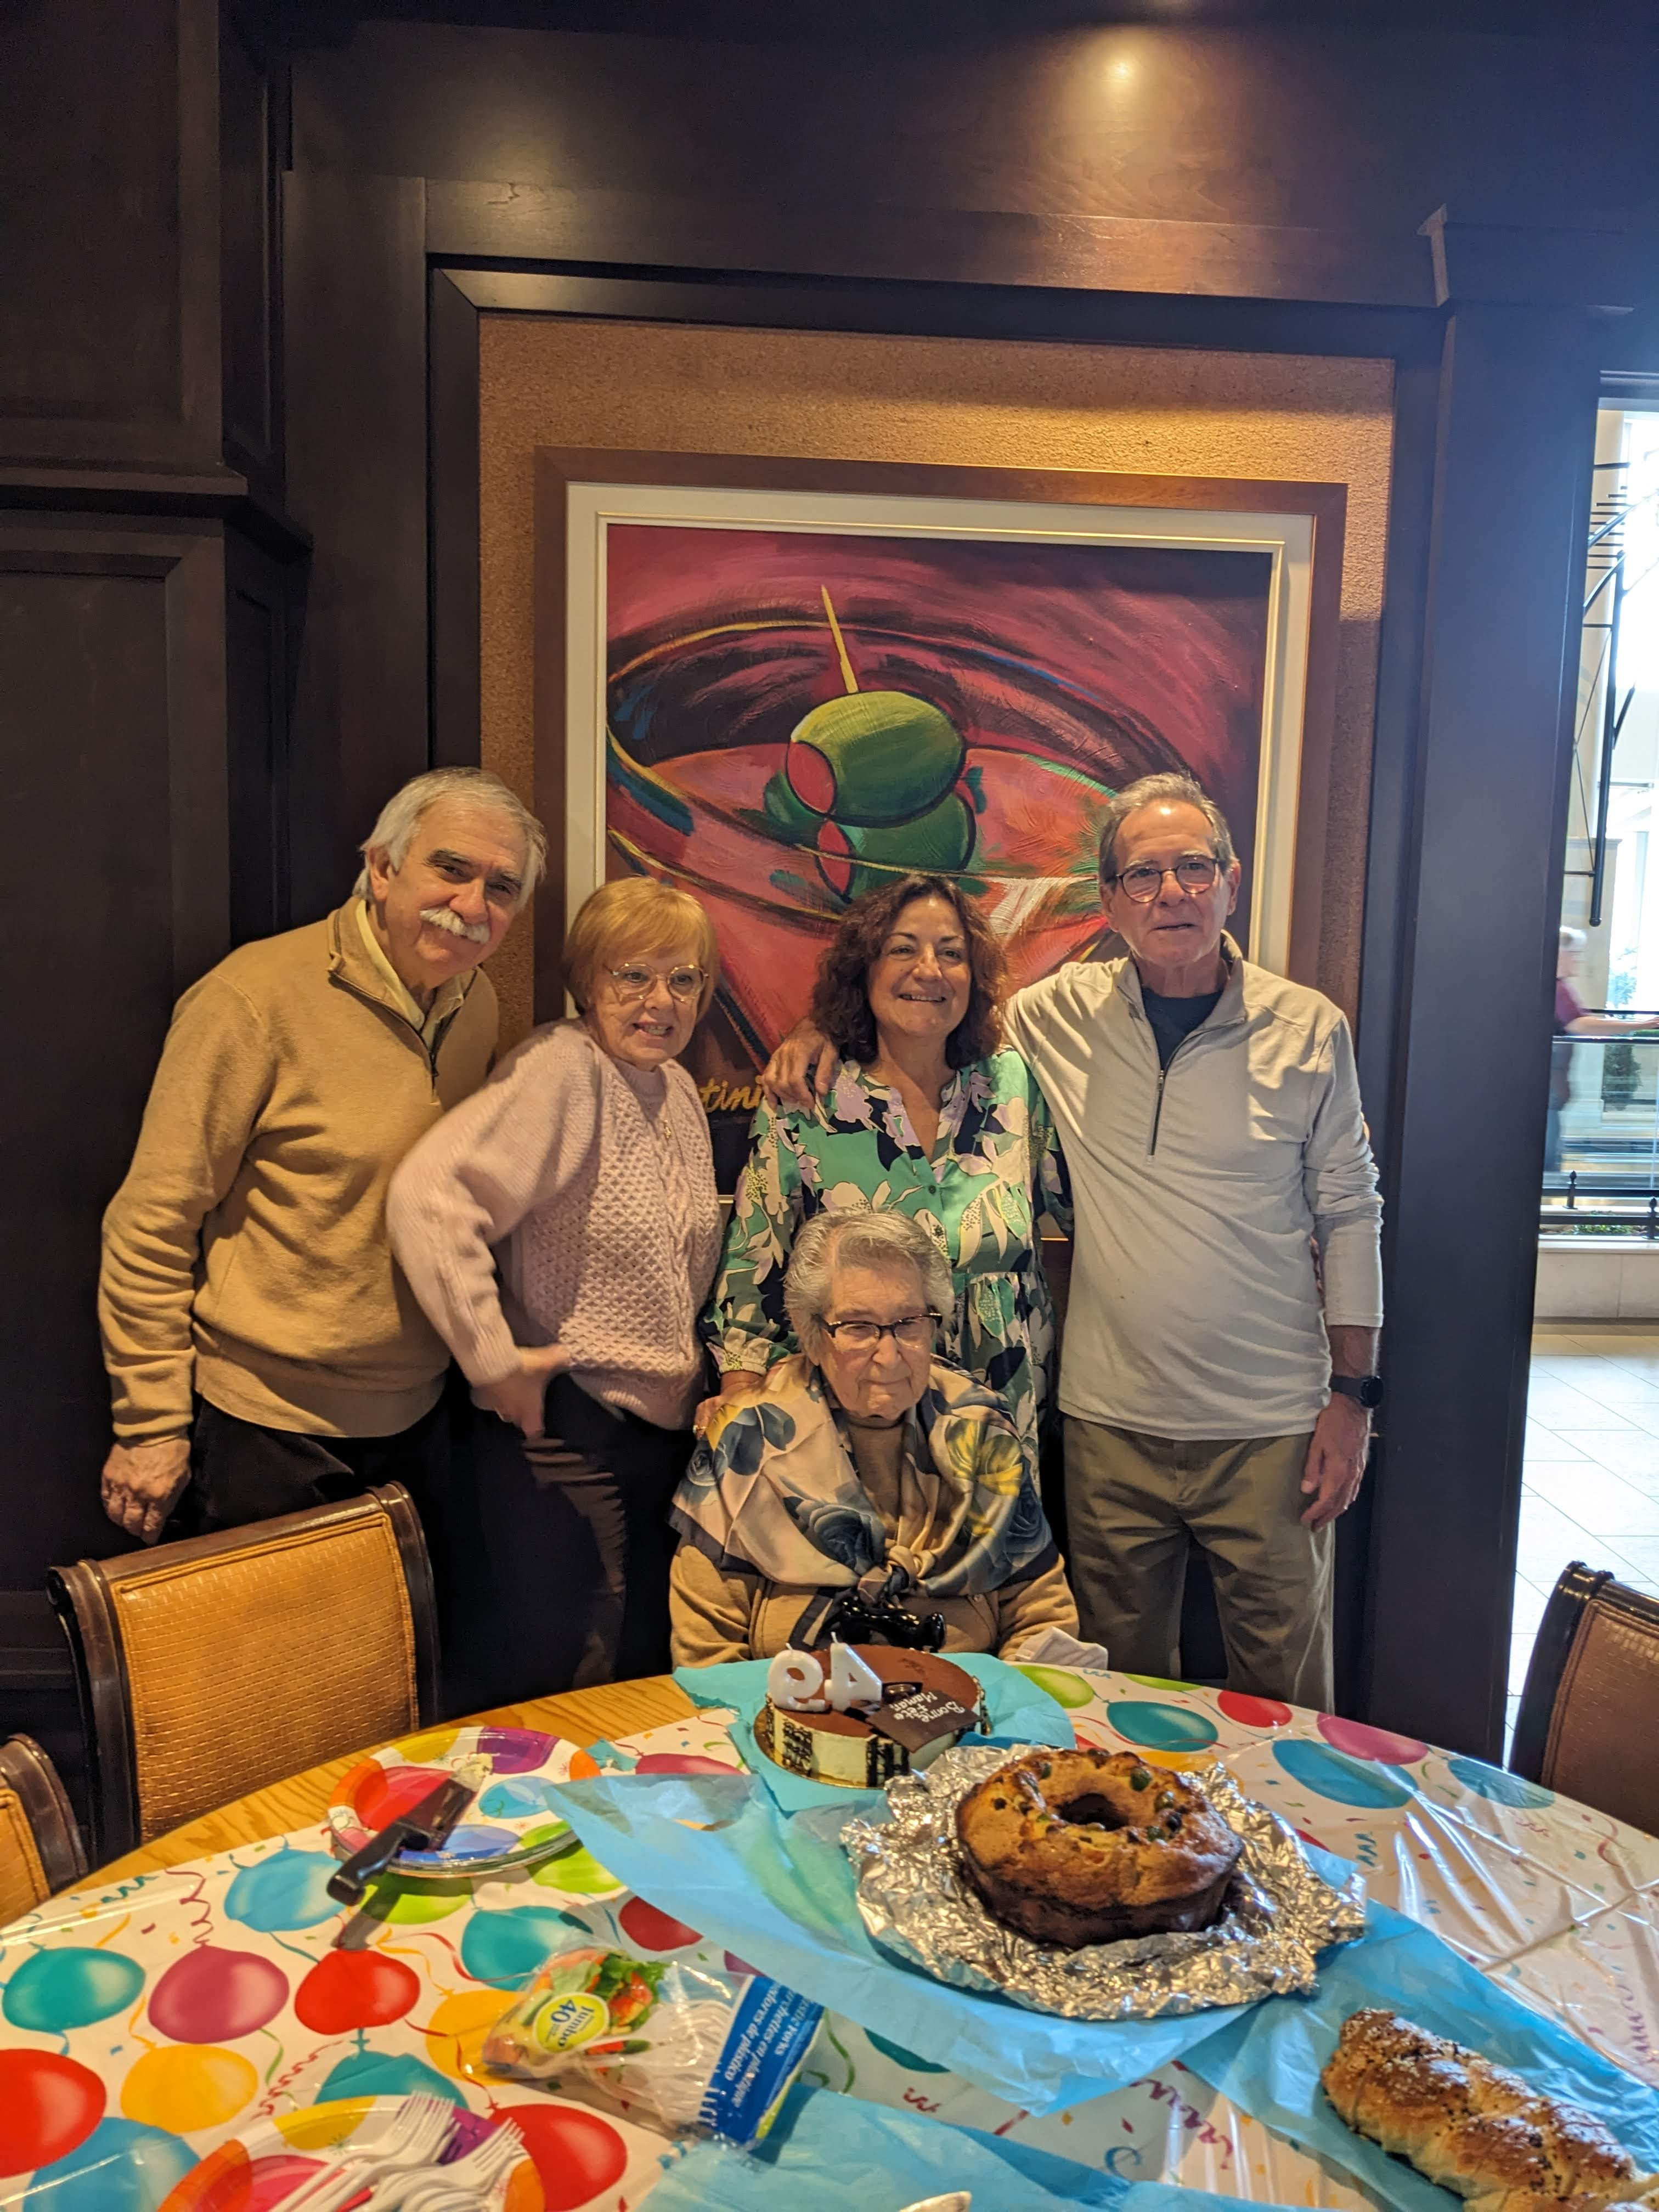
\includegraphics[width=70mm]{dermardiros/images/Ciambalone.jpg}
%     \caption{Grandma Lucie's birthday in 2024}
% \end{figure}

\captionfigure{dermardiros/images/Ciambalone.jpg}{Grandma Lucie's birthday in 2024}{fig:ciambalone}


\chapter{The Best Chewy Chocolate Chip Cookies}
\label{ch:chocolatechip_cookies}
\index{dessert}
\index{cookies}
\index{chocolate}

\marginnote{
    \textbf{Makes 12~cookies} \\
    Prep time: 20~minutes \\
    Cook time: 12-15~minutes \\
    \vspace*{\baselineskip}

    ½~cup granulated sugar (100~g) \\
    ¾~cup brown sugar, packed (165~g) \\
    1~tsp salt
    ⅓~cup unsalted butter, melted (113~g) \\
    1~large egg \\
    1~tsp vanilla extract \\
    1¼~cups all-purpose flour (155~g) \\
    ½~tsp baking soda \\
    4~oz milk or semi-sweet chocolate chunks (110~g) \\
    4~oz dark chocolate chunks (110~g), or your preference
}

\marginalfigure{dermardiros/images/Ballon poire 2023.jpg}{Ballon poire at Clara's birthday, 2023}{fig:chocolatechip_cookies2}

Family member: Emma

\begin{enumerate}
    \item Preheat oven to 350\degree F or 180\degree C.
    \item Bake for 12-15~minutes.
\end{enumerate}

\captionfigure{dermardiros/images/Dzovag's cookies written by Emma.jpeg}{Handwritten recipe}{fig:chocolatechip_cookies}

\chapter{Banana Cake}
\label{ch:bananacake}
\index{dessert}
\index{cake}
\index{banana}

\marginnote{
    \textbf{Makes 1~loaf} \\
    Prep time: 20~minutes \\
    Cook time: 45~minutes \\
    \vspace*{\baselineskip}

    3~ripe bananas \\
    6~tbsp vegetable oil \\
    ½~cup sugar \\
    1~egg \\
    1~tsp vanilla extract\\
    ¼~tsp salt \\
    1½~cups all-purpose flour \\
    1~tsp baking soda \\
    1~tsp baking powder
}

Family member: Dzovag

\marginalfigure{dermardiros/images/Christmas girls.jpg}{Christmas, 2021}{fig:bananacake}

\begin{enumerate}
    \item Preheat oven to 350\degree F.
    \item In a bowl, mix the bananas and vegetable oil together.
    \item Add the sugar, egg, vanilla extract and salt. Mix well.
    \item In another bowl, mix the flour, baking soda and baking powder. Add the dry ingredients to the other bowl containing the wet ingredients.
    \item Once well mixed, pour into a greased loaf pan.
    \item Bake for 12-15~minutes.
\end{enumerate}

% \include{dermardiros/cheureg}  % images in \dermardiros\images
\restoregeometry

\part{Monanteras Family}
\chapter{Potatoes with Eggs}
\label{ch:eggswithpotatoes}
\index{eggs}
\index{potatoes}
\index{dinner}
\index{breakfast}

\marginnote{
    \textbf{Makes 4+ servings} \\
    Prep time: 15~hours \\
    Cook time: 20~minutes \\
    \vspace*{\baselineskip}

    Potatoes \\
    Eggs \\
    Olive oil \\
    Mitzithra or Pecorino romano, grated
}

\textit{Patates me avga}

Family member: Grandma Elisavet

\newthought{Grandma Elisavet} would make \textgreek{πατάτες με αυγά} often for my dad and uncle when they were little. It was a meal that was easily put together and can sustain you for hours! Everytime we would visit our house in Dara, grandma would always have a place ready for us when we arrived because she knew we had travelled a long way and were hungry.

\begin{enumerate}
    \item Peel and cut the potatoes into wedges. Place them in a bowl of cold water.
    \item Heat a large frying pan, add some olive oil. When hot, add the potatoes and fry them. Once cooked, remove and set them aside on a plate.
    \item Add the eggs to the hot pan, mix them while they cook (scramble them).
    \item As the eggs cook, add back the potatoes. Continue mixing with a spatula while the eggs cook.
    \item Put the potatoes and eggs onto a large place and sprinkle lots of grated cheese. Serve warm!
\end{enumerate}

\twosidecaptionfigure{monanteras/images/Dara.pdf}{monanteras/images/Grandma elisavet.jpg}{(Left) The house, (Right) In front of the house in Dara, Tripoli}{fig:eggswithpotatoes}

\chapter{Fakes}
\label{ch:fakes}
\index{meal}
\index{lentils}
\index{soup}

\marginnote{
    \textbf{Makes 6-8~servings} \\
    Prep time: 30~minutes + overnight soaking \\
    Cook time: 2~hours \\
    \vspace*{\baselineskip}
    
    2½~cups green lentils, dry \\
    1~white onion \\
    3~tbsp olive oil \\
    2~garlic cloves, thinly sliced \\
    1~can tomato sauce, Hunt's (213~ml) \\
    3~bay leaves \\
    1~pinch salt \\
    Carrots, sliced (optional) 
}

\textit{Lentil soup}

Family member: Mom

\begin{enumerate}
    \item Soak lentils in cold water overnight (around 12~hours). The next day, drain out the water using a sieve.
    \item In a medium pot, grate onion and add 3~tbsp olive oil.
    \item Heat on high and cook until the onion is soft. Add drained lentils and cook.
    \item Add the tomato sauce. Bring the pot over the sink and fill half the pot with water.
    \item Continue heating, add the bay leaves, salt, garlic and carrots if using. Bring to a boil and reduce heat to Medium to keep to a simmer.
    \item Simmer until the soup thickens and lentils are cooked, about 1~hour and 30~minutes.
\end{enumerate}

Eat with toasted sourdough bread and a piece of feta! Normally we halve this recipe and add paprika and pepper for taste. You can also add the garlic while browning the onions.

\chapter{Fassolakia}
\label{ch:fassolakia}
\index{meal}
\index{green beans}
\index{tomato}

\marginnote{
    \textbf{Makes 8+ servings} \\
    Prep time: 15-20 minutes \\
    Cook time: 1-2 hours \\
    \vspace*{\baselineskip}

    1 large onion, chopped \\
    1 bag green beans \\
    1 can tomato sauce, Hunt's (213ml) \\
    1/2 cup parsley, chopped \\
    Salt \\
    Oil \\
    3-5 red potatoes, peeled and quartered (keep in cold water)
}

\textit{Green beans with potatoes}

Family member: Mom

\marginalfigure{monanteras/images/Green beans 1.jpg}{Fassolakia}{fig:fassolakia}

\begin{enumerate}
    \item Wash green beans and remove both edges.
    \item Drizzle a little of oil in a large pot, add onion once heated. Cook on medium heat.
    \item When the onion is translucent, add the green beans and mix. Add the tomato sauce, stir and add water until all the beans are covered.
    \item Add chopped parsley, salt and mix.
    \item Bring to a boil and keep it simmering uncovered until the beans are softened, about 45 minutes.
    \item Add the potatoes and keep cooking. Add a little water if necessary to cover potatoes.
    \item When you can poke the potatoes with a knife and the sauce has reduced, remove the pot from the heat and cover. Let cool for about 1 hour before eating.
\end{enumerate}

Eat with a large piece of feta and village bread!

\chapter{Mavromatika}
\label{ch:mavromatika}
\index{meal}
\index{spinach}
\index{beans}

\marginnote{
    \textbf{Makes 6 servings} \\
    Prep time: 20 minutes \\
    Cook time: 2 hours + overnight soaking \\
    \vspace*{\baselineskip}

    1/2 mug of black eyed peas, dried (or 1/2 cup) \\
    1 medium onion, grated \\
    1/2 - 1 can tomato sauce, Hunt’s (213 ml) \\
    2 bags of spinach, fresh \\
    Olive oil 
}

\textit{Spinach stew with black eye peas}

Family member: Mom

\begin{enumerate}
    \item Soak black eyed peas in water overnight.
    \item The next day, drain the water. Put them in a pot with water and bring them to a simmer. Cook for about 20-30 minutes until almost done and strain.
    \item In a large pot, bring water to a boil. Add spinach and cook until soft, for about 15 minutes. Strain the spinach on top of the black eyes peas.
    \item Heat a medium pot and add oil. Cook onion until softened, then add the beans and the spinach. Add the tomato sauce, 2 cans of water, salt and pepper.
    \item Simmer until reduced and thickened. During cooking, you can add more water if thickens too much, to get desired consistency.
    \item After about 1 hour to 1 hour and a half, check the beans for doneness, then turn off heat and let cool.
\end{enumerate}

To speed things up, I would use 1 can of black eyed peas and skip Steps 1 and 2. It is quicker to make and would take a total of 45 min to cook.

Also really good with, you guessed it, a slice of village bread and a large piece of feta!

\chapter{Kolokithokeftedes}
\label{ch:kolokithokeftedes}
\index{side}
\index{zucchini}
\index{feta}

\marginnote{
    \textbf{Makes 16~patties} \\
    Prep time: 20~minutes \\
    Cook time: 30~minutes \\
    \vspace*{\baselineskip}

    4~zucchinis, grated \\
    4~tbsp fresh mint, chopped \\
    1~cup green onions, chopped \\
    3~tbsp parsley, chopped \\
    ¾~cup feta, crumbled \\
    2~eggs \\
    2~tsp cumin \\
    ½~tsp pepper \\
    1~tsp garlic powder \\
    ¾ - 1~cup breadcrumbs \\
    1~tbsp oil
}

\marginalfigure{monanteras/images/Zucchini fritter.jpg}{Kolokithokeftedes}{fig:kolokithokeftedes}

\textit{Zucchini fritters}

Family member: Grandma Eleni

\begin{enumerate}
    \item Squeeze out the excess water from the zucchinis using a towel.
    \item In a large bowl, add all the ingredients and mix. Start by adding ¾~cup of the breadcrumbs, and add more if the mix is wet and sticky.
    \item Shape into 3-inch patties.
    \item Lightly flour the patties and fry until golden brown.
\end{enumerate}

Best eaten warm, next to grilled meat.

\chapter{Hilopites with Chicken}
\label{ch:hilopites}
\index{meal}
\index{chicken}
\index{pasta}

\marginnote{
    \textbf{Makes 6-8~servings} \\
    Prep time: 15-30~minutes \\
    Cook time: 2~hours \\
    \vspace*{\baselineskip}

    1~large onion \\
    1~garlic clove \\
    About 11~chicken drumsticks, without skin \\
    Salt \\
    Pepper \\
    ½~can tomato sauce, Hunt's, 213~ml, or 1~full can \\
    1~tbsp tomato paste, optional \\
    1~cup hilopites, or orzo/pasta
}

\textit{Homemade egg pasta in broth with chicken}

Family member: Mom

\newthought{Grandma} \textgreek{Ελισσάβετ} makes \textgreek{χυλοπήτες} every summer in Greece and brings them to us when she comes back to Canada. Mom would make this dish with grandma's homemade, but you can find \textgreek{χυλοπήτες} at Greek supermarkets like Marché PA and Atlantis.

\begin{enumerate}
    \item In a large pot, grate the onion and add some olive oil. Heat on high.
    \item When it starts to sizzle, stir with a wooden spoon and add the chicken drumsticks. Season with salt and pepper and stir until chicken is lightly browned.
    \item Add the ½~or 1~can of tomato sauce and tomato paste, if using.
    \item Add about 3~cups of water, mix and reduce heat.
    \item Cook for 1½~hours until reduced and left with about 2~cups liquid.
    \item Remove the chicken and while keeping liquid on a simmer, add the hilopites.
    \item Add another ½~cup water and cook on a low simmer for 10-15~minutes until the hilopites are cooked. Can add a little more water if too thick.
    \item Once hilopites are cooked and soup has thickened, remove from the heat and add back the chicken.
\end{enumerate}

Serve with lots of grated Romano or Parmesan. Can also make the hilopites without chicken.

\chapter{Oven Roasted Chicken with Potatoes}
\label{ch:chickenandpotatoes}
\index{meal}
\index{chicken}
\index{potatoes}

\marginnote{
    \textbf{Makes 4 servings} \\
    Prep time: 25 minutes \\
    Cook time: 1 hour and 30 minutes \\
    \vspace*{\baselineskip}

    1 whole chicken, cut in half with the neck removed \\
    1-2 lemons, squeezed \\
    4-5 red potatoes, peeled and quartered, put in water \\
    Carrots, bell peppers, onions, peeled and sliced \\
    Olive oil \\
    Salt \\
    Pepper \\
    Oregano \\
    Paprika
}

Family member: Mom

\begin{enumerate}
    \item In a large pan, place chicken flat down.
    \item In a large bowl, add the sliced potatoes and season with salt, pepper, oregano, paprika and olive oil. Toss the potatoes to coat them well, and add them to the chicken.
    \item Add what ever vegetables you like to the pan: carrots, bell peppers, onions.
    \item Add about 2 cups of water and the lemon juice. Sprinkle everything with salt, pepper, oregano and paprika, drizzle with olive oil.
    \item Bake at 350\degree F for 1 hour to 1 hour and a half, or until you can pierce the potatoes with a fork. Add more lemon juice or water if necessary.
\end{enumerate}

\chapter{Meat Sauce}
\label{ch:meatsauce}
\index{meal}
\index{meat}
\index{pasta}

Family member: Mom

\marginnote[20pt]{\\
    \textbf{Makes 6+ servings} \\
    Prep time: 20 minutes \\
    Cook time: 2 hours \\
    \vspace*{\baselineskip}

    1650 g ground beef, extra lean \\
    1 jar of Catelli Garden Select Tomato \& Basil Pasta Sauce (640ml) \\
    1 can tomato juice, Heinz (540 ml) \\
    1 onion, diced \\
    Salt and pepper \\
    Olive oil \\
    Pecorino cheese, Chelmos Greek or other \\
    \vspace*{\baselineskip}
}

\begin{figure}
    \includegraphics[width=60mm]{monanteras/images/Meatsauce no cheese.jpg}
    \includegraphics[width=60mm]{monanteras/images/Meatsauce with cheese.jpg}
\end{figure}

\marginnote{
    We found that using 650g of ground beef, half the jar of Catelli and half the tomato juice can, makes enough for 2 people (with lots of leftovers). It took us a little over an hour to cook half the quantity - Elsa \& Vaski
}

\begin{enumerate}
    \item Heat oil in a medium to large sized saucepot and cook the onion.
    \item Add the minced meat and cook well, until browned. Add the tomato juice, salt and pepper. Using the Heinz tomato juice can, add 2 cans of water to the pot and stir. Cover the pot and allow to cook over medium heat for approximately 1 hour.
    \item When the sauce has thickened and is almost ready, add the jar of Catelli Garden Select and stir very well. Cover the pot and let it cook for 30-45 minutes.
    \item The sauce is ready when it starts to thicken. Boil your pasta: add 1 tsp of salt to a pot of boiling water and prepare the spaghetti according to the instructions on the package.
    \item Top with meat sauce and sprinkle with lots of pecorino cheese. ENJOY :)
\end{enumerate}

\chapter{Lasagna}
\label{ch:lasagna}
\index{meal}
\index{pasta}
\index{meat}
\index{cheese}

\marginnote{
    \textbf{Makes 8+ servings} \\
    Prep time: 30-45 minutes \\
    Cook time: 35 minutes \\
    \vspace*{\baselineskip}

    \textbf{One recipe of Meat sauce, page~\pageref{ch:meatsauce}} \\
    \vspace*{\baselineskip}

    454 g (1 pkg) Ricotta cheese \\
    285 g (1 pkg) frozen chopped spinach, thawed and drained \\
    2 eggs, lightly beaten \\
    500 g lasagna noodles, Primo (around 12 sheets) \\
    1 jar of Catelli Garden Select Tomato \& Basil Pasta Sauce (640ml) \\
    Shredded mozzarella cheese \\
    Grated Pecorino cheese, Chelmos Greek or mitzithra
}

Family member: Mom

\newthought{Lasagna} was a comforting dinner Mom used to make on Sundays. We would get yelled at for eating the top layer of pieces (: You can omit the ricotta \& spinach layer if you want and make it a very meat and cheesy lasagna!

\begin{enumerate}
    \item Preheat oven to 350\degree F and grease a 9~x~13-inch ovenproof dish with Pam spray.
    \item Cook the lasagna noodles according to the package instructions. Once done, set aside.
    \item In a bowl, mix the ricotta cheese, eggs and spinach.
    \item Spread a thin layer of Garden Select Pasta Sauce, approximately 4 tbsp, in the bottom of the ovenproof dish. Top with 4 lasagna sheets or more, enough to cover the whole bottom of the dish.
    \item Top with the prepared meat sauce. Add another 2 tbsp of the Pasta Sauce on top and sprinkle with 2 tbsp of Pecorino cheese.
    \item Top with the lasagna sheets. On top, spread all of the prepared spinach mixture and top with more sheets of lasagna.
    \item Top with more meat sauce, 2 tbsp of Pasta Sauce on top and another 2 tbsp of Pecorino cheese.
    \item Top with lasagna noodles and remaining meat sauce. Sprinkle enough shredded mozzarella to cover all the meat sauce and some more of the Pecorino cheese.
    \item Bake for 35-45 minutes, or until the top is golden and bubbly and the corners are crusty. Let cool before cutting into slices! Enjoy :)
\end{enumerate}

Leave the frozen spinach on the counter for a few hours to defrost. Squeeze out the liquid as much as you can before adding it to the egg and ricotta.


\chapter{Gemista}
\label{ch:gemista}
\index{meal}
\index{rice}
\index{vegetables}
\index{meat}

\marginnote{
    \textbf{Makes 8+ servings} \\
    Prep time: 45 minutes \\
    Cook time: 1 hour \\
    \vspace*{\baselineskip}
    
    ? g ground beef, extra lean \\
    ? long grain rice, rinsed \\
    6 medium-sized tomatoes \\
    2 red bell peppers \\
    2 green bell peppers \\
    2 garlic cloves \\
    1 cup olive oil \\
    1 cup fresh parsley, chopped \\
    1 cup fresh mint, chopped \\
    1 can tomato juice, Heinz (540 ml) \\
    1 large onion, thinly chopped \\
    4 red potatoes, peeled and cut into wedges \\
    Breadcrumbs \\
    Salt, pepper and oregano \\
    Grated Pecorino cheese, Chelmos Greek
}

\textit{Tomatoes and peppers stuffed with meat and rice}

Family member: Mom

\newthought {Gemista} are vegetables stuffed with rice, minced meat and herbs cooked with potatoes in a tomato sauce. They are usually made with tomatoes, bell peppers, zucchini, eggplants... My grandmother even stuffed potatoes because I didn't like vegetables as a child! \textgreek{Καλή όρεξη}!

% \begin{figure}
%   \includegraphics[width=60mm]{monanteras/images/Cooked gemista.jpg}
% \end{figure}

\marginalfigure{monanteras/images/Cooked gemista.jpg}{Gemista}{fig:gemista}

\begin{enumerate}
    \item Preheat oven to 350\degree F and grease a 9X13-inch ovenproof dish with Pam spray.
    \item Wash the tomatoes and remove the stems. Slice the tops off each tomato, leaving a bit of flesh attached. Carefully remove the flesh out of each tomato and place it into a bowl. Place each one of the tomatoes into the prepared baking dish and place their tops aside.
    \item Cut the top of the peppers, clean the inside of each and place them in the baking dish, place their tops aside.
    \item Heat 1/2 cup of olive oil in a pot and cook the onion. Once softened, add the garlic and stir well. Add the minced meat, rice, parsley and mint, and stir well. Season with salt and pepper, and cook until the meat has browned. Add the insides of the tomatoes and 1/2 can of Heinz tomato juice. Stir well.
    \item Using a spoon, stuff the tomatoes and the peppers until a little below the rim and cover with their tops. Arrange the sliced potatoes around the \textgreek{Γεμιστά}.
    \item Pour the remaining 1/2 can of tomato juice as well as 1/2 cup water in the pan. Drizzle the other 1/2 cup olive oil over the tomatoes and potatoes. Season with salt, pepper and oregano. Add some breadcrumbs and grated Pecorino cheese on the tops.
    \item Bake in the preheated oven uncovered for 60-70 minutes, or until the tomatoes are golden on top. The potatoes should be easily pierced with a knife.
\end{enumerate}


\chapter{Roasted Lamb and Potatoes}
\label{ch:lambpotatoes}
\index{meal}
\index{lamb}
\index{Easter}

\marginnote{
    \textbf{Makes 8+ servings} \\
    Prep time: 45~minutes \\
    Cook time: 1½ - 2~hours \\
    \vspace*{\baselineskip}

    1~leg of lamb \\
    Salt \\
    Pepper \\
    3~cloves of garlic, chopped \\
    Olive oil \\
    Oregano \\
    2~lemons, juiced \\
    4~red potatoes, peeled and quartered
}

Family member: Mom \& Dad

\begin{enumerate}
    \item Preheat oven to 350\degree F.
    \item Prepare the leg of lamb: cut the leg into pieces or leave it whole and add it to a large bowl.  Add olive oil, salt, freshly ground pepper and oregano on all its sides, and toss it well. Pierce the leg with a knife and put the pieces of garlic inside. Place the lamb in a large baking dish or roasting pan.
    \item In a bowl, toss the potatoes with olive oil, salt, pepper and oregano and add them to the baking dish.
    \item Pour the lemon juice on the lamb and potatoes, then add 1~cup of water.
    \item Place in the oven uncovered for 1~hour and a half, or until the potatoes are soft and can be pierced easily with a knife. You can add 30~minutes to make sure there the top of the lamb is crispy!
\end{enumerate}

\twosidecaptionfigure{monanteras/images/Lamb.jpg}{monanteras/images/Lamb 2.jpg}{(Left) Lamb before putting it in the oven, (Right) Lamb after cooking}{fig:lambpotatoes}

% \chapter{The Chocolate Cake}
\label{ch:chocolatecake}
\index{dessert}
\index{cake}
\index{chocolate}

\marginnote{
    \textbf{Makes 1 cake} \\
    Prep time: ? minutes \\
    Cook time: ? minutes \\
    \vspace*{\baselineskip}

    \textbf{Ingredients for cake} \\
    3 eggs \\
    227g butter (1/2 block) \\
    1 cup milk \\
    2 cups sugar \\
    3 cups all-purpose flour, ? \\
    3 tbsp cocoa powder
    1 tbsp baking powder \\
    Vanilla extract \\
    Zest of 1 orange \\

    \textbf{Ingredients for chocolate ganache} \\
    3 cups sugar
    2 cups water

    \textbf{Ingredients for syrup} \\
    1 cup water \\
    1 cup sugar \\
    1 tbsp lemon juice
}

\textit{A Very Chocolatey Cake with Syrup and Maraschino Cherries}

Family member: Grandma Eleni

% {{{ The follwing is from ChatGPT, to be updated...
\begin{enumerate}
    \item Preheat the oven to 180°C (350°F). Grease and flour a 9-inch cake pan.
    \item In a mixing bowl, cream the butter and sugar until light and fluffy. Add the eggs one at a time, beating well after each addition.
    \item Mix in the vanilla extract and orange zest.
    \item Sift together the flour, cocoa powder, and baking powder. Gradually add the dry ingredients to the wet mixture, alternating with the milk. Mix until just combined.
    \item Pour the batter into the prepared pan and bake for 45 minutes, or until a toothpick inserted in the center comes out clean.
    \item While the cake is baking, prepare the syrup. In a saucepan, combine water, sugar, and lemon juice. Bring to a boil, then simmer for 5 minutes. Set aside to cool.
    % this one doesn't make sense... but the chocolate ganache also is missing ingredients
    \item For the ganache, heat the cream in a saucepan until just about to boil. Remove from heat and pour over chopped dark chocolate. Let sit for 5 minutes, then stir until smooth.
    \item Once the cake is baked, allow it to cool slightly, then poke small holes all over the surface with a skewer. Drizzle the syrup evenly over the cake.
    \item Spread the ganache over the top and sides of the cake. Decorate with maraschino cherries or as desired.
\end{enumerate}

Grandma Eleni's cake is always a hit at family gatherings, with its moist texture and rich chocolate flavor.
% }}}

\twosidecaptionfigure{monanteras/images/Chocolate cake 2.jpg}{monanteras/images/Chocolate cake.jpg}{(Left) Celebrating Grandma's 80$^{th}$ birthday, (Right) The Chocolate Cake}{fig:chocolatecake}

\chapter{Easter Koulourakia}
\label{ch:easter_koulourakia}
\index{dessert}
\index{cookies}
\index{Easter}

\marginnote{
    \textbf{Makes 45 cookies} \\
    Prep time: 20-30 minutes \\
    Cook time: 12-15 minutes \\
    \vspace*{\baselineskip}

    4 cups all-purpose flour (Five Roses preferably) \\
    3 eggs, separated \\
    1 1/4 cups sugar \\
    3/4 cup butter, unsalted, melted and cooled \\
    1 tsp ammonia powder \\
    2 tsp baking powder \\
    3/4 tsp vanilla powder (or 1 tsp vanilla extract) 
}

\textit{The White Cookies}

Family member: Grandma Eleni

\marginalfigure{monanteras/images/Easter koulourakia.jpg}{Easter koulourakia}{fig:easter_koulourakia}

\newthought{Grandma} \textgreek{Ελένη} would make \textgreek{κουλουράκια} every Easter. They are best eaten soon after baking with a coffee or dipped in milk. Since she made a large batch, she would keep them stored in Tupperwares, which made them soft. We all preferred them that way!

\begin{enumerate}
    \item In a large bowl, mix the flour with the baking powder and vanilla powder (if using).
    \item In bowl, beat the egg whites with a small amount of sugar using a mixer to obtain a meringue. Place in the fridge.
    \item Warm milk, remove from the heat and add ammonia powder. Stir until it foams and set it aside. Be careful - it smells strong!
    \item Using a mixer, beat the egg yolks with the remaining sugar, slowly add the melted butter and foamy milk/ammonia while mixing. Using a spatula, fold in the egg whites.
    \item Slowly add the dry ingredients to the wet ingredients, add as much as the dry as needed (normally use 3 1/2 - 4 cups).
    \item Mix with a spatula (or hands), scrape the sides of the bowl. Add very little oil to hands and mix with hands to form a dough. It should unstick from the bowl.
    \item Shape into balls, then thin ropes and twists, pretzels and koulouria.
    \item Place on baking sheets lined with parchment, brush with the reserved egg yolks and sprinkle with almond flakes.
    \item Bake at 350\degree F for 8 minutes, turn the baking sheet and for another 6-8 minutes.
\end{enumerate}

% \begin{figure}
%   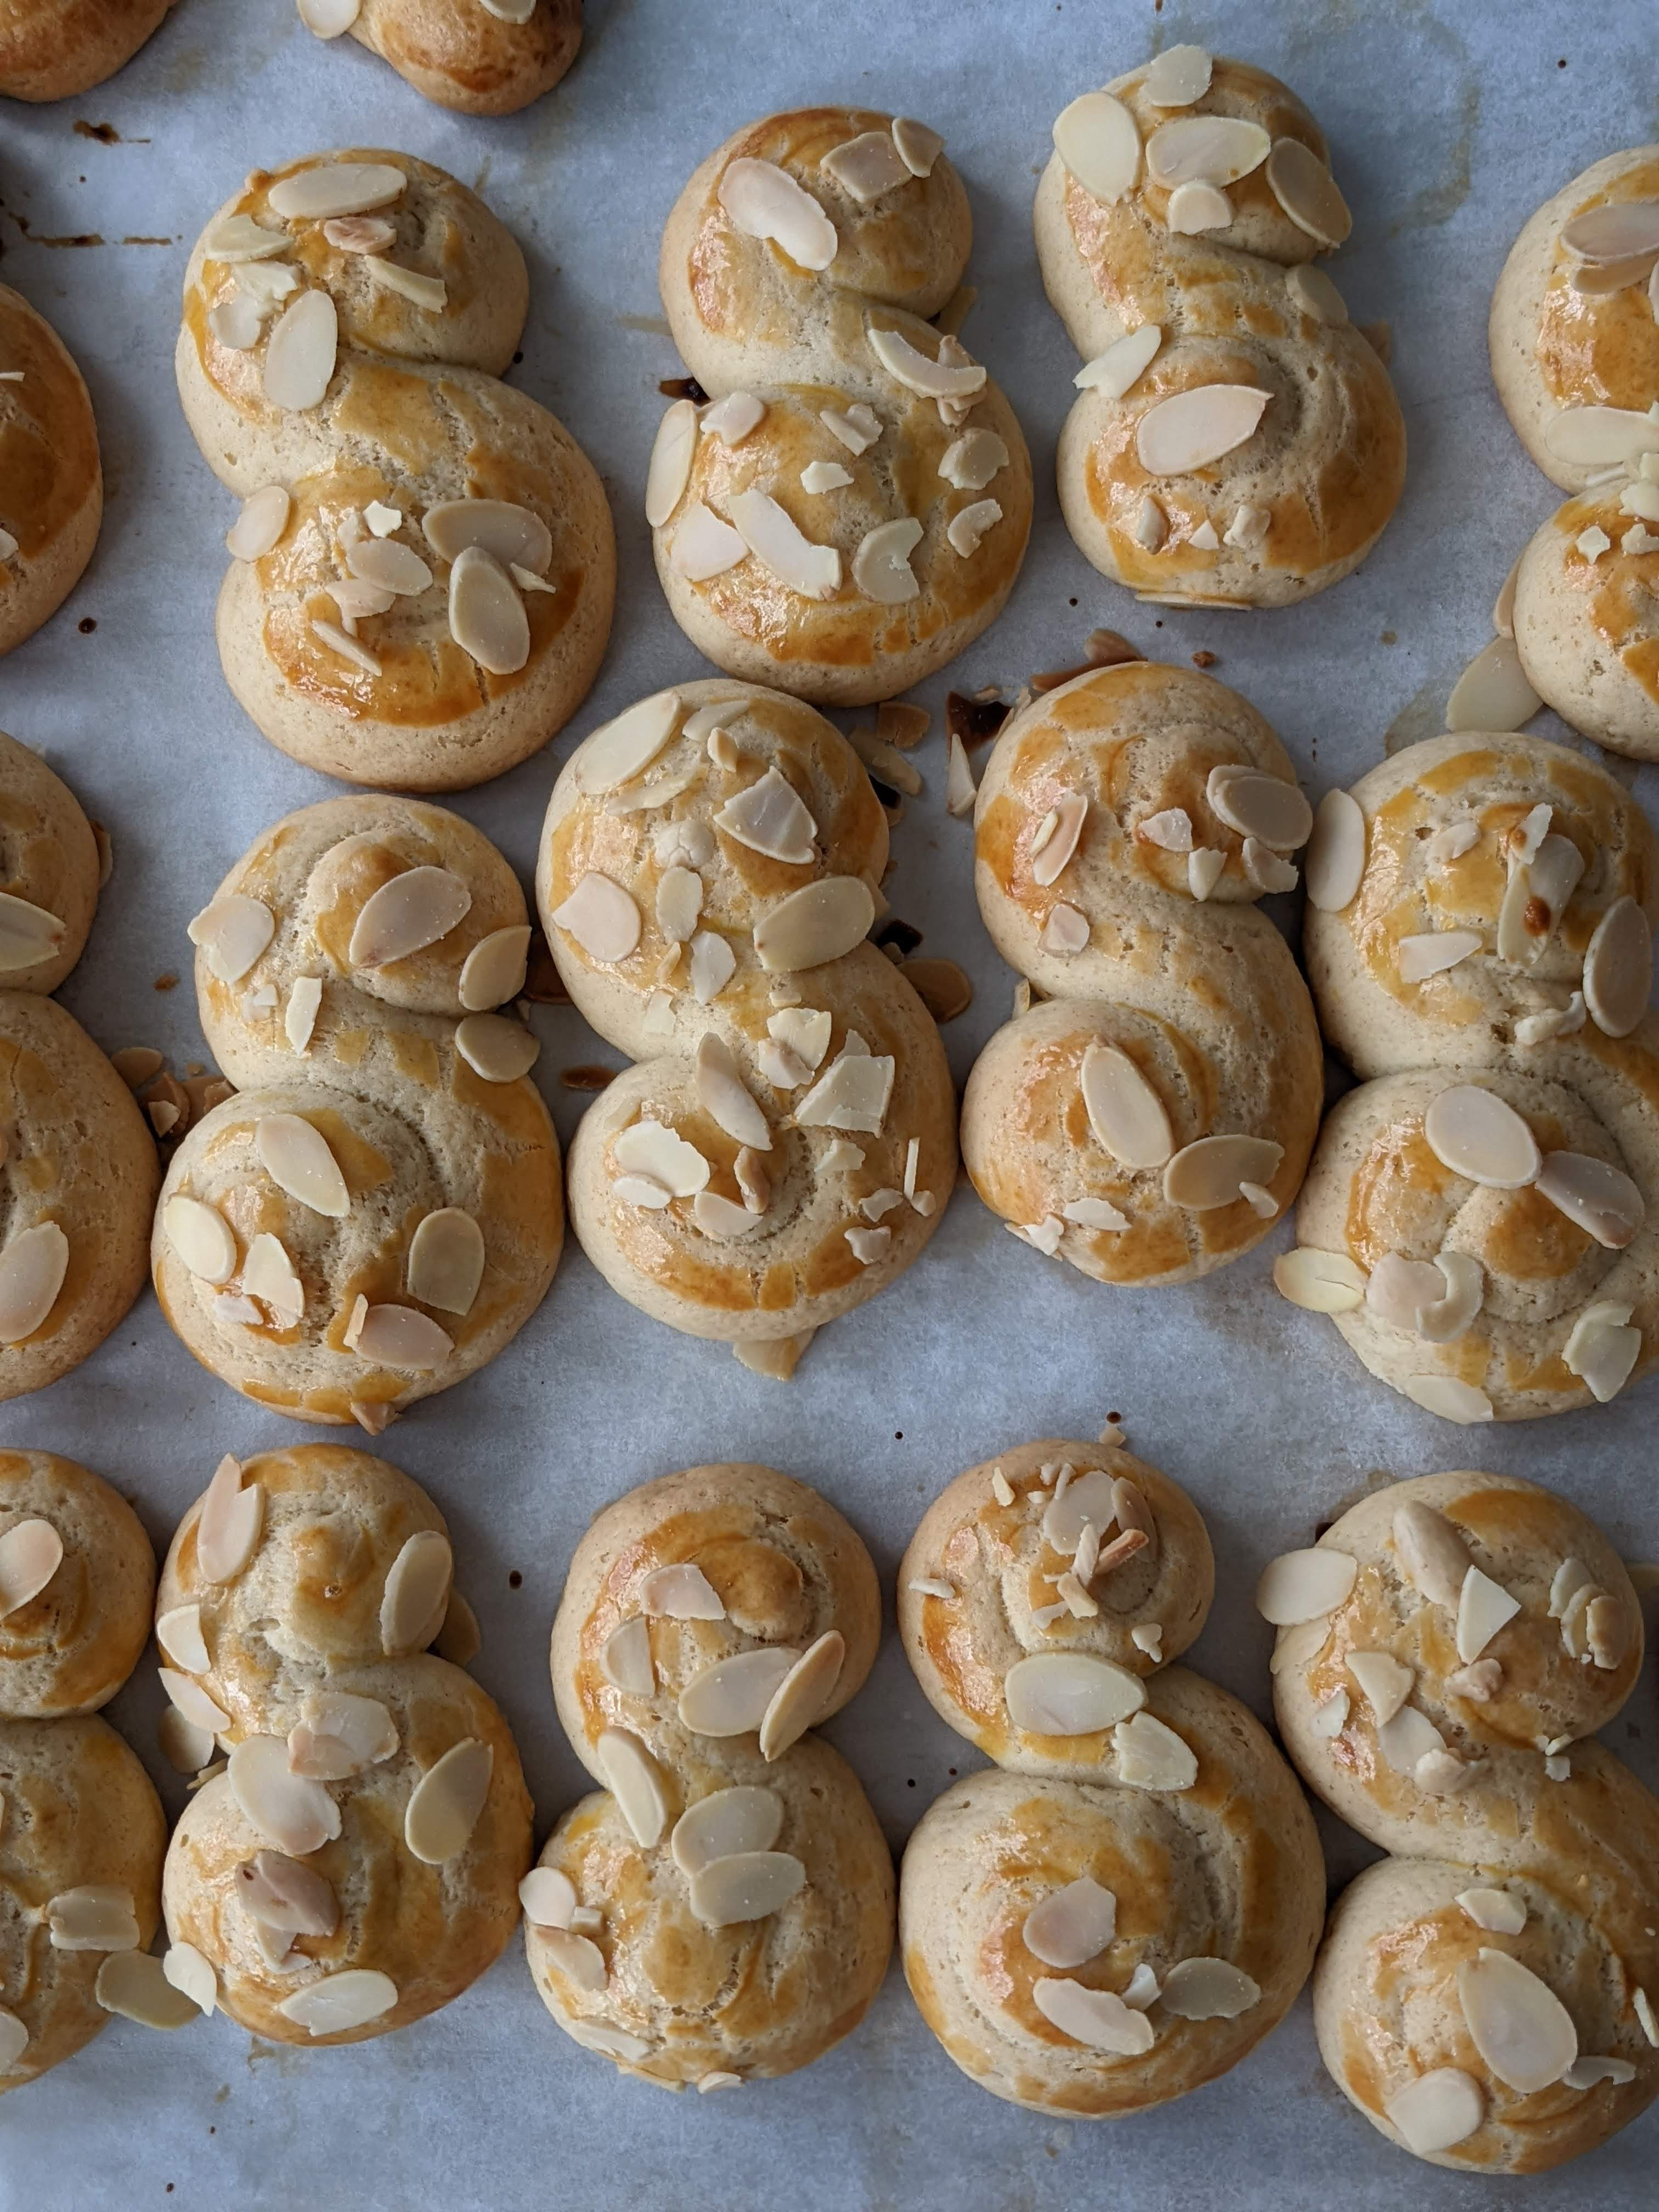
\includegraphics[width=60mm]{monanteras/images/Easter koulourakia.jpg}
% \end{figure}
%
% \begin{figure}
%   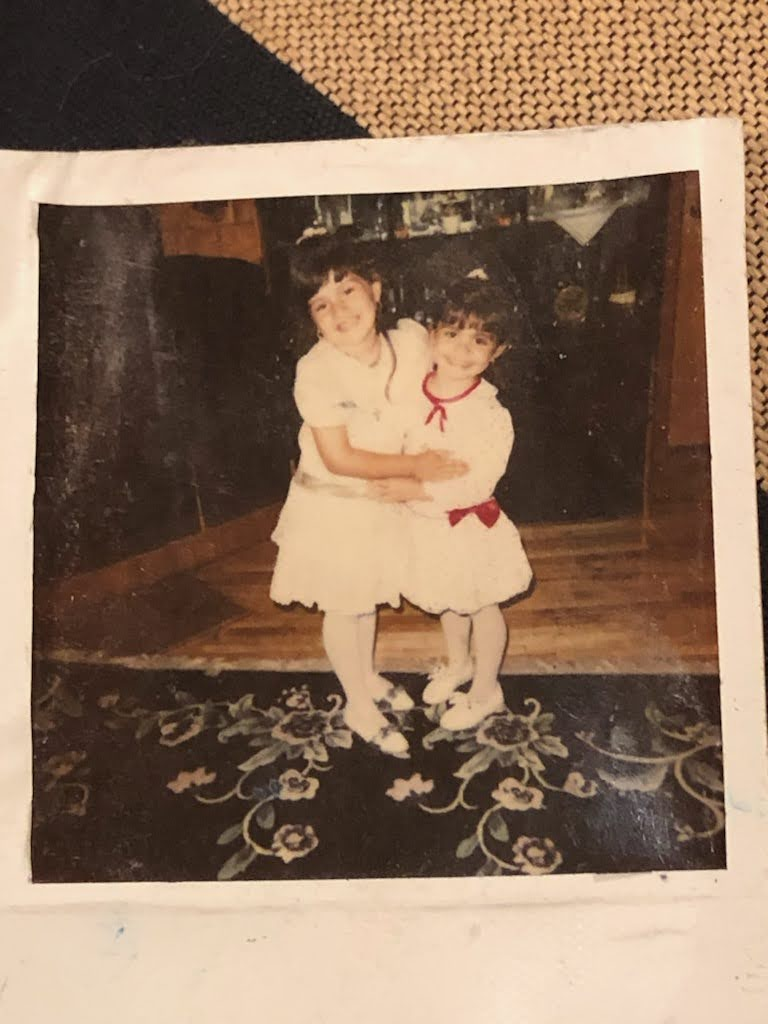
\includegraphics[width=60mm]{monanteras/images/IMG_20241009_171710.jpg}
%   \caption{Us in our Easter outfits, with our white Easter shoes}
% \end{figure}

\captionfigure{monanteras/images/IMG_20241009_171710.jpg}{Elsa and Helen in Easter outfits, with white Easter shoes!}{fig:easter_koulourakia_2}


\chapter{Painted Easter Eggs}
\label{ch:eastereggs}
\index{Easter}

\marginnote{
    \textbf{Makes 48 painted eggs} \\
    Prep time: 10 minutes \\
    Cook time: 20 minutes \\
    \vspace*{\baselineskip}

    \textbf{Ingredients for cookies} \\
    48 eggs \\
    1 pack of Red Dye for Eggs, Rida \\
    1/2 cup vinegar \\
    Vegetable oil
}

Family member: Mom

\marginalfigure{monanteras/images/Eggs 7.jpg}{Red Easter eggs}{fig:eastereggs}

\newthought{After every} Easter dinner we would all gather around the table to break the painted eggs. At the end, we would have egg shell on the entire table and our hands would be red! And every year, a different person would have the "strongest" egg!     The dye can be found at Greek bakeries such as at Afroditi or Serano Bakery in Laval. Mom found this method to yield the deepest red colored eggs.

\begin{enumerate}
    \item Boil the eggs and cool them.
    \item Empty the color in the pot filled with 1 liter of lukewarm water and the vinegar.
    \item Add enough eggs to be fully covered with the colored water. After 5 minutes, remove the eggs and place them on paper towel to drain the water.
    \item Wipe the eggs with some vegetable oil.
    \item Using the same colored water, do the same with the rest of the eggs.
\end{enumerate}

\twosidecaptionfigure{monanteras/images/Easter eggs with grandma.jpg}{monanteras/images/Eggs 3.jpg}{Easter with Grandma Eleni}{fig:eastereggs_2}
\twosidecaptionfigure{monanteras/images/Eggs 5.jpg}{monanteras/images/Eggs 4.jpg}{Big batch of Easter eggs}{fig:eastereggs_3}

% \chapter{Moustokouloura}
\label{ch:moustokouloura}
\index{dessert}
\index{cookies}
\index{molasses}

\marginnote{
    \textbf{Makes 48 cookies} \\
    Prep time: 2-3 hours \\
    Cook time: 12-15 minutes \\
    \vspace*{\baselineskip}

    4 1/2 cups all-purpose flour, sifted \\
    1/2 tsp cinnamon \\
    1/2 tsp cloves \\
    1 tsp baking powder \\
    1 tsp ammonia powder \\
    2 eggs \\
    3/4 cup sugar \\
    1/2 vegetable oil \\
    1/2 orange juice (fresh is better) \\
    1/2 cup molasses
}

\textit{The brown cookies}

Family member: Grandma Eleni

\newthought{The Brown Cookies} is what we called these cookies. Since \textgreek{μούστο} (grape must) was not easy to find in Canada, Grandma \textgreek{Ελένη} replaced it with molasses. They are a bit tricky to shape, so use some vegetable oil on your hands while shaping.

\begin{enumerate}
    \item In a bowl, mix the cinnamon, cloves, baking powder and ammonia. Add about half of the flour and whisk together. Keep the other flour aside.
    \item In a large mixing bowl, beat the eggs with the sugar. Slowly add the oil, orange juice and molasses while beating.
    \item Add the dry ingredients (half the flour with the spices and baking powder) to the wet ingredients slowly while mixing. Scrape down the sides of the bowl, and let the dough rest for about 15 min.
    \item Restart the mixer and add some of the flour that was kept aside, as much as needed to form a ball. You might not have to use it all.
    \item Place a little bit of vegetable oil in a small bowl and use it to wet hands. Use hands to knead the dough slightly. Dough might be sticky, but use some oil to wet hands. Roll into small balls then into strings, then shape into twists, pretzels and small koulourakia.
    \item Place the shaped cookies onto baking sheets and bake 12-15 minutes on the upper rack at 350\degree F until the tops have a golden color.
\end{enumerate}

Eat soon after baking, and once cooled, stored in a large Tupperware. This allows them to be soft and can be kept for a long time if you can resist.

\twosidecaptionfigure{monanteras/images/Moustokouloura.jpg}{monanteras/images/Moustokouloura recipe.jpg}{Moustokouloura}{fig:moustokouloura}

\chapter{Karidopita}
\label{ch:karidopita}
\index{dessert}
\index{cake}
\index{walnut}

\marginnote{
    \textbf{Makes ?} \\
    Prep time: ? minutes \\
    Cook time: ? minutes \\
    \vspace*{\baselineskip}

    \textbf{Ingredients for cake} \\
    2 1/2 cups all-purpose flour (Monarch Cake \& pastry flour **put picture**) \\
    8 eggs \\
    2 cups sugar \\
    1 cup gingerale \\
    1 cup walnuts \\
    1 cup vegetable oil \\
    1 tsp baking soda \\
    1 tsp baking powder \\
    1/2 tsp cinnamon \\
    1/2 tsp cloves \\
    \vspace*{\baselineskip}

    \textbf{Ingredients for syrup} \\
    3 cups sugar \\
    2 cups water 
}

\textit{Walnut cake with syrup}

Family member: Grandma Eleni

\newthought{Helen} made this recipe for a work lunch and everyone was obsessed with them!

\begin{enumerate}
    \item In a large bowl, mix all the ingredients for the cake using a whisk. Leave the gingerale for last.
    \item Pour into a 12~x~18 inch sized metal pan. Bake at 350\degree F for ? minutes.
    \item While cake is baking, make the syrup. Put the sugar and water in a medium pot and mix. Heat until it simmers and let it boil for 5 minutes. Remove from the heat and let it cool.
    \item Once the cake is done and has a golden colour, remove from the oven. Pour all of the cooled syrup onto the warm cake.
    \item Let the cake cool and cut into diamond shapes.
\end{enumerate}

% TODO:
Koupa used by grandma for this recipe is equivalent to ? ml.


\chapter{Portokalopita}
\label{ch:portokalopita}
\index{dessert}
\index{cake}
\index{orange}

\marginnote{
    \textbf{Makes 15 servings} \\
    Prep time: 45 minutes \\
    Cook time: 50 minutes - 1 hour \\
    \vspace*{\baselineskip}

    \textbf{Ingredients for cake} \\
    450g phyllo sheets (1 pack) \\
    4 eggs \\
    3/4 cup sugar \\
    Zest from 2 oranges \\
    1 cup Greek yogurt \\
    1/4 tsp salt \\
    1 tsp baking soda \\
    1 tsp baking powder \\
    1 cup vegetable oil \\
    1/2 cup orange juice, freshly squeezed \\
    1 tsp vanilla extract \\
    Vegetable oil for greasing the baking pan
    \vspace*{\baselineskip}

    \textbf{Ingredients for syrup} \\
    1 1/2 cups sugar \\
    1 1/2 cups water \\
    1/3 cup orange juice \\
    1 cinnamon stick \\
    1/4 tsp orange blossom water, optional 
}

\textit{Orange Phyllo Cake}

Family member: Helen

\newthought{Another recipe} Helen made for a work potluck. Approved by her Greek manager who loves this dessert!

\begin{enumerate}
    \item Start by drying out the phyllo. Preheat the oven to 200\degree F. Open up the phyllo sheets, and one by one, scrunch them up, starting from the short side. After scrunching a sheet, place it on a baking pan and do the same with the entire pack of phyllo. You will need 2 baking sheets to for all the phyllo. Bake them in the middle and bottom racks of the oven for 10 minutes. After the 10 minutes, flip the phyllo sheet over and bake for an additional 8 minutes. Turn off the oven, keep the oven door open slightly and leave the phyllo in the oven to dry it out. Once completely dry use your hands to crumble the phyllo into small pieces, and set them aside.
    \item Meanwhile, prepare the syrup: combine the water, sugar, orange juice, cinnamon stick and orange blossom water in a pot. Bring them to a boil, then reduce the heat to a simmer. Simmer for 15 minutes then let it cool.
    \item Preheat the oven to 350\degree F. In the large mixing bowl, beat the eggs and the sugar for 3-4 minutes, until it is a pale yellow colour.
    \item Add the orange zest, Greek yoghurt, vanilla extract, baking powder, baking soda and salt, and mix until just combined.
    \item Add the oil and the orange juice to the bowl, and mix to combine well with the rest of the ingredients.
    \item Using a rubber spatula begin to incorporate your dried out and torn phyllo into the cake batter, a little bit at a time.
    \item Pour the mixture into a 9x13 inch sized baking dish (Pyrex). Bake for 50-60 minutes.
    \item Once the cake is done and has a golden color, remove from the oven. Immediately pierce it in several places with a long clean souvlaki stick. \item Pour all of the cooled syrup onto the warm cake, one ladle at a time. Allow each ladle to be absorbed into the cake before adding the next one. Repeat until all of the syrup has been used.
    \item Let the cake cool before cutting, to allow the syrup to be fully absorbed.
\end{enumerate}

\begin{figure}
  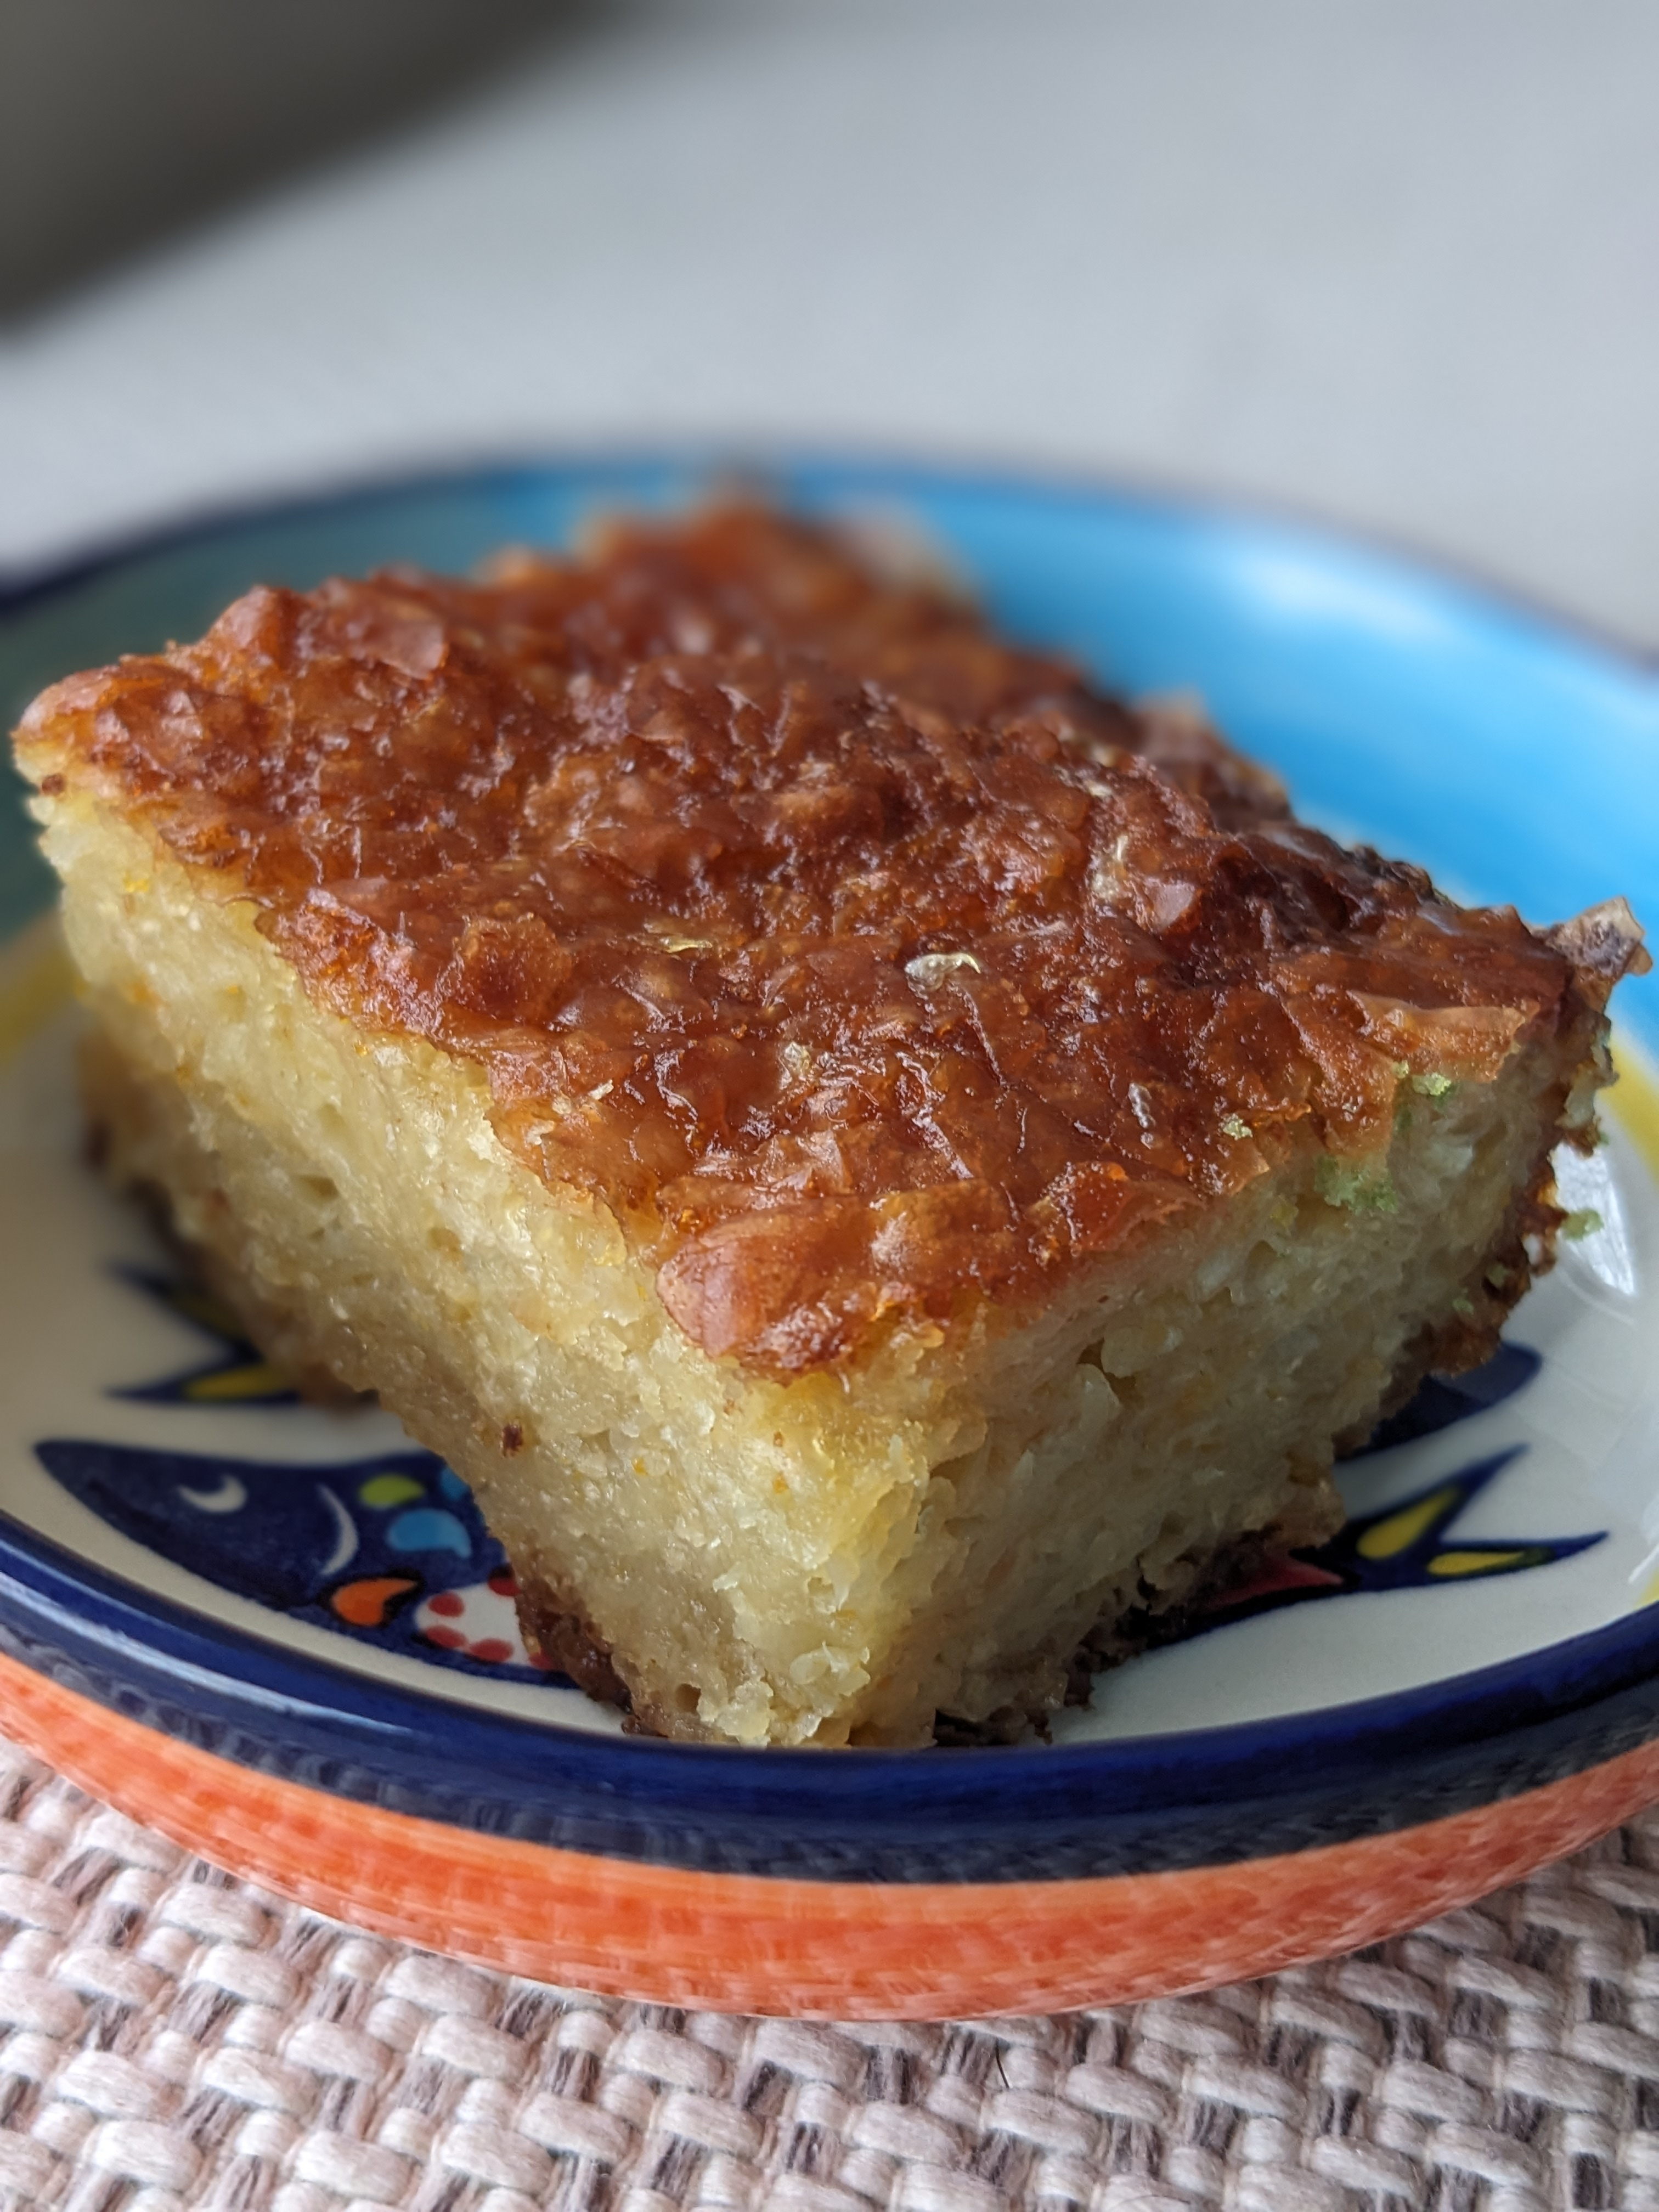
\includegraphics[width=60mm]{monanteras/images/portokalopita.jpg}
\end{figure}
\begin{figure}
  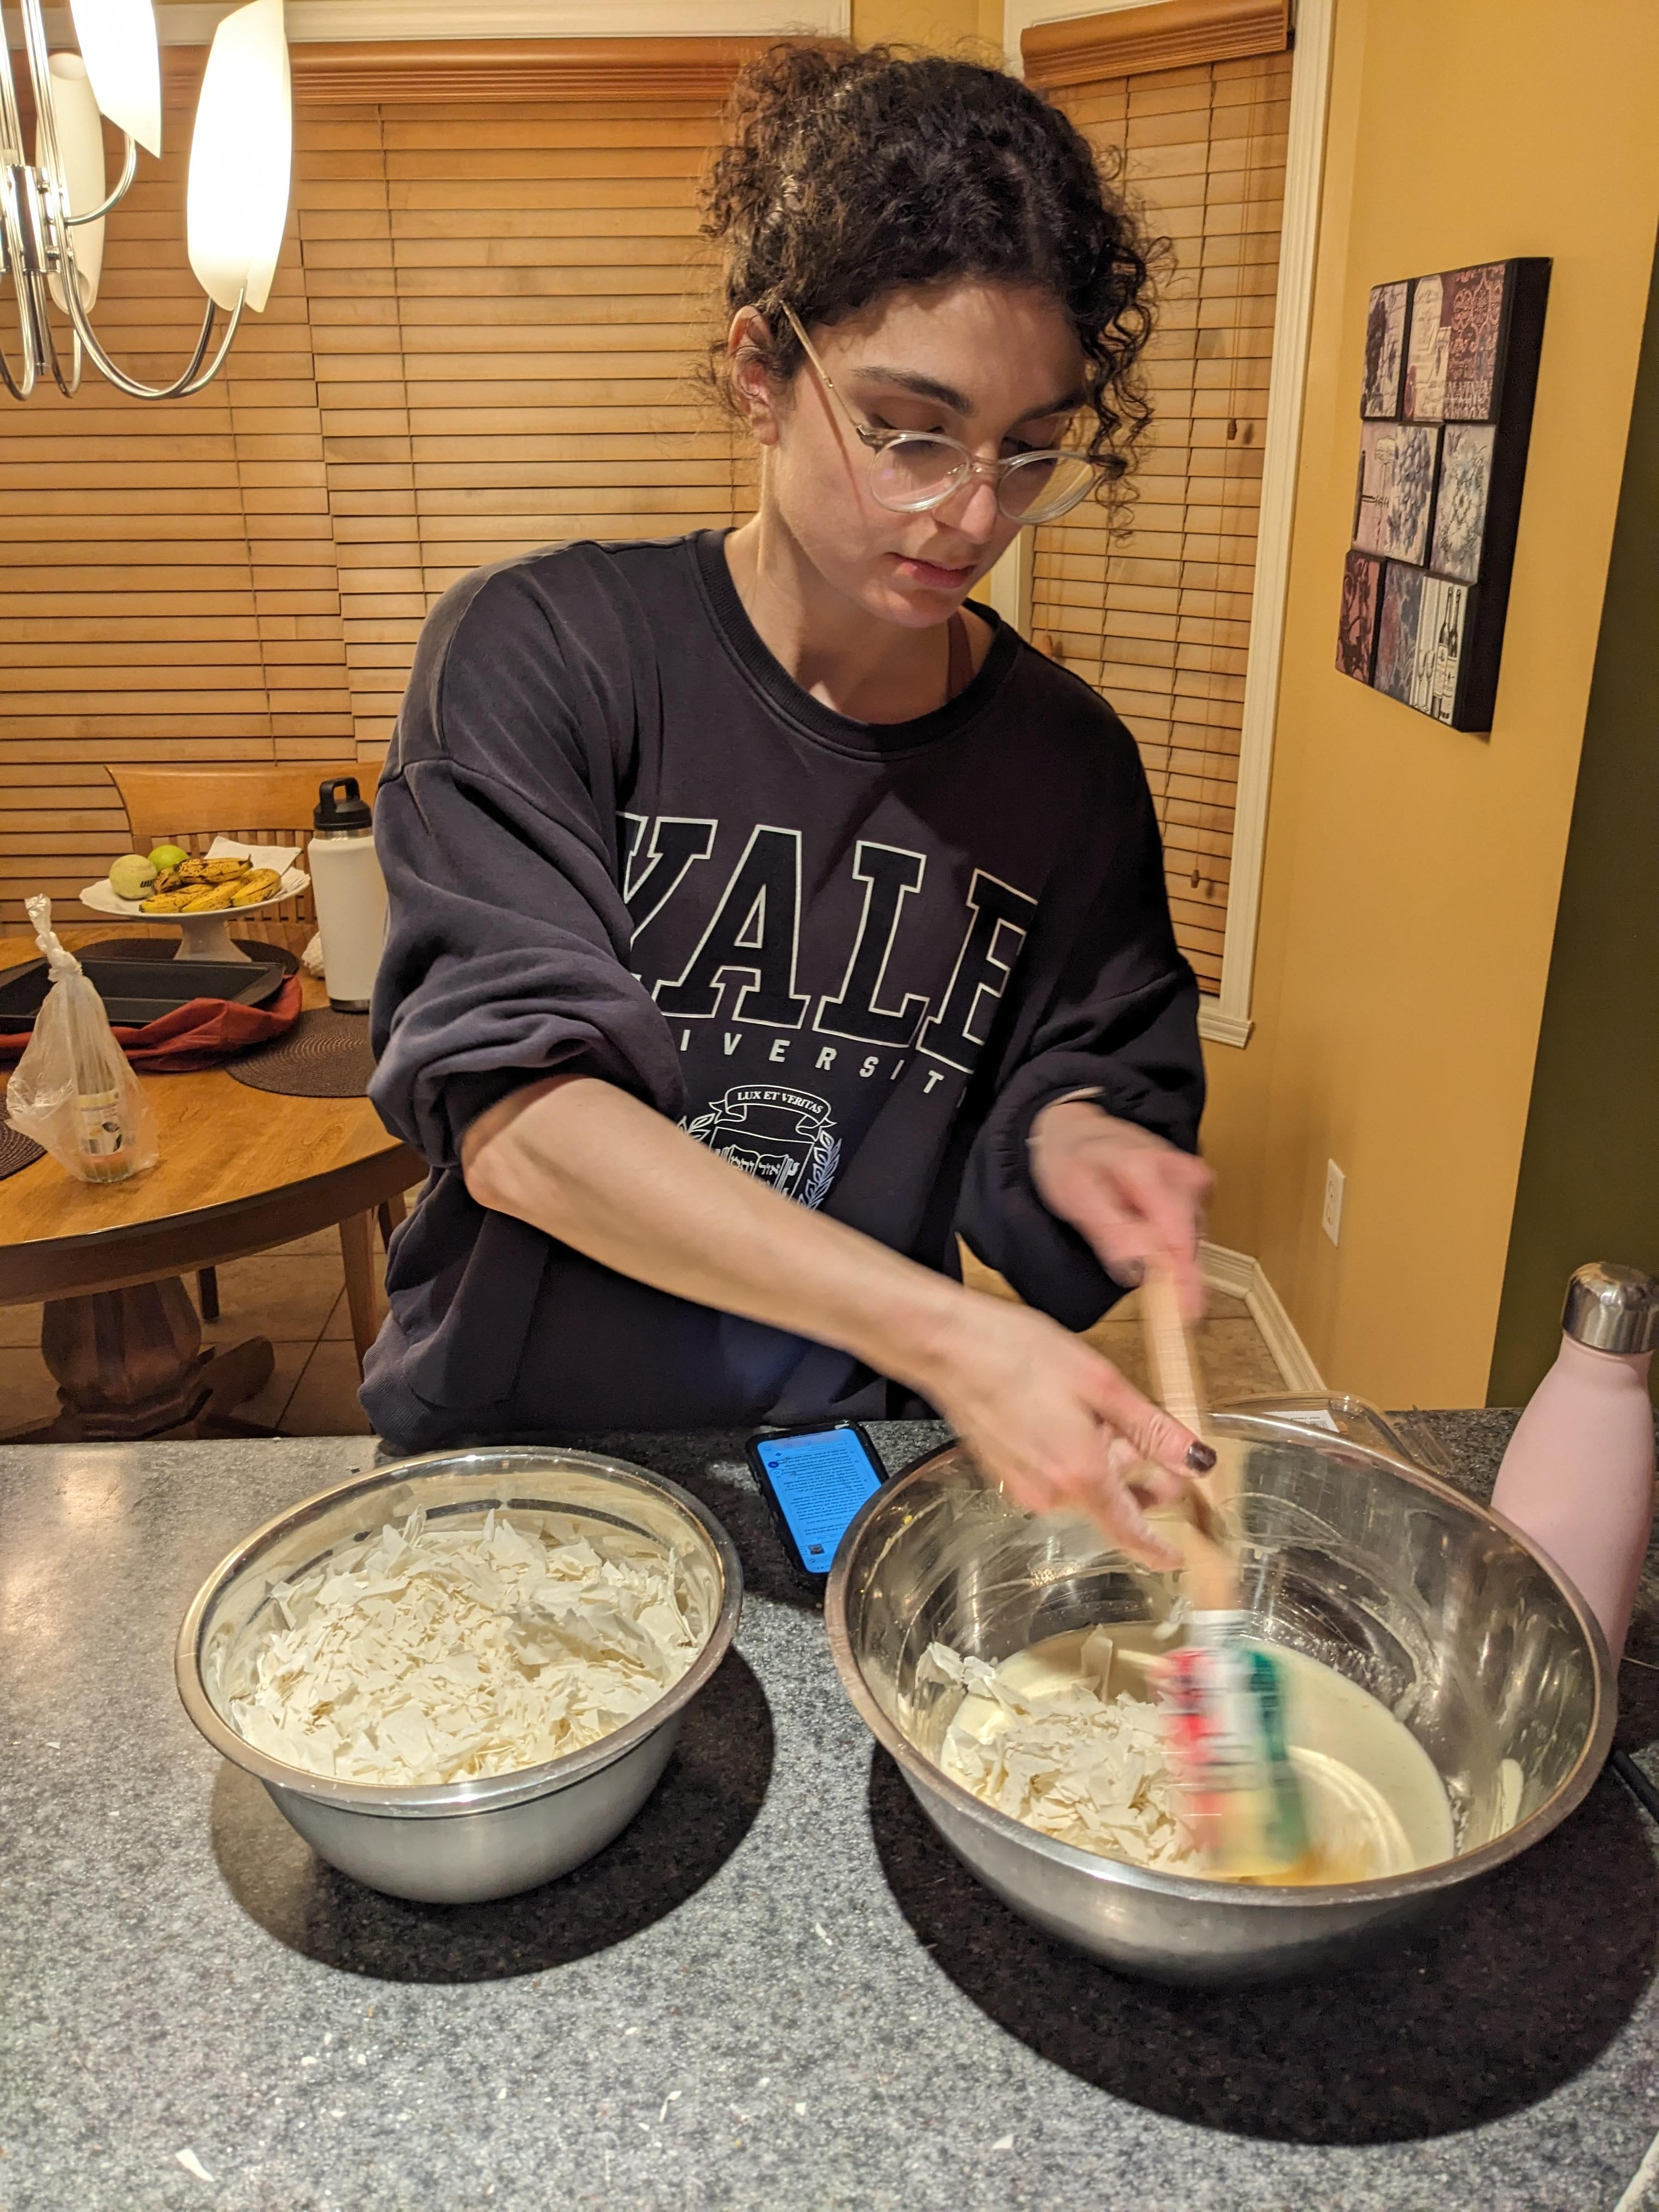
\includegraphics[width=60mm]{monanteras/images/portokalopita2.jpg}
\end{figure}

You can decorate each piece of portokalopita with slices of oranges or keep it simple. Gets better with time :)


\chapter{Melomakarona}
\label{ch:melomakarona}
\index{dessert}
\index{cookies}
\index{walnut}
\textit{Honey Cookies with Walnuts and Syrup}

Family member: Grandma Eleni

\marginnote[20pt]{\\
    \textbf{Makes ? cookies} \\
    Prep time: ? minutes \\
    Cook time: 30 minutes \\
    \vspace*{\baselineskip}

    \textbf{Ingredients for cake} \\
    7 cups all purpose flour, Five Roses
    3 cups vegetable oil
    1/2 cup sugar \\
    1/2 cup orange juice, freshly squeezed \\
    1/2 cup beer \\
    2 tsp cinnamon \\
    1 tsp cloves \\
    3 tsp baking powder \\
    \vspace*{\baselineskip}
    
    \textbf{Ingredients for syrup and decoration} \\
    Greek honey \\
    1/2 cup sugar \\
    1/2 cup water \\
    Walnuts, crushed \\
}

\begin{enumerate}
    \item In a large bowl, mix all the ingredients for the melomakarona. Start with 6 cups flour, and add more to get texture needed to shape.
    \item Place the shapes melomakarona on a baking sheet. Bake at 350\degree F for about 30 minutes or until slightly golden.
    \item Once the cookies are done and have a golden color, remove from the oven. Let the cookies cool. 
    \item To make the syrup, put the ingredients in a medium pot and mix. Heat until it simmers and let it boil for 5 minutes. Remove from the heat.
    \item Once the cookies have cooled, put the warm syrup in a large bowl. Dip the cookies one by one, on both sides with a fork in the syrup. Place them on a cooling rack for excess syrup to drip
    \item Decorate with crushed walnuts before storing them in a large Tupperware.
\end{enumerate}

\marginnote{Koupa used by grandma for this recipe is equivalent to ? ml.}
\chapter{Diples}
\label{ch:diples}
\index{dessert}
\index{honey}
\index{Christmas}

\marginnote{
    \textbf{Makes 12+ servings} \\
    Prep time: 45~minutes \\
    Cook time: 1~hour \\
    \vspace*{\baselineskip}

    4~eggs \\
    4~small water glasses of sugar \\
    Flour, all-purpose, as much as the dough takes \\
    Greek honey \\
    Walnuts, crushed \\
    Cinnamon
}

\marginalfigure{monanteras/images/Diples.jpg}{Diples from a bakery in the town of Levidi, Arcadia}{fig:diples}

\textit{Greek honey dipped fried pastries}

Family member: Grandma Elisavet

\newthought{Every Christmas} my grandma would make \textgreek{δίπλες}. A traditional Greek dessert from the Peloponnessos, diples are light and airy fried dough dipped in honey, walnuts and dusted with cinnamon. They can be kept for 1-2~weeks in a plastic container, lined with plastic wrap.

\begin{enumerate}
    \item In a large bowl, mix the eggs with the sugar.
    \item Add flour, and mix until you can form a dough, mix slowly. If too stiff, add water bit by bit. If too soft, add some flour.
    \item Using a rolling pin, roll out the dough until you have thin sheets. Cut them into strips, then rectangles.
    \item Heat oil in a frying pan. One by one, fry the dough sheets. When they start to puff up, use a fork to roll them and form a cylinder. Once they start to colour, remove them onto a plate lined with paper.
    \item Warm honey in a small pot. Once the diples have cooled down, drizzle some honey on top, add crushed walnuts and a sprinkle of cinnamon. Serve with coffee after Christmas dinner!
\end{enumerate}

\chapter{Lemon Cake}
\label{ch:Lemoncake}
\index{dessert}
\index{cake}
\index{lemon}

\marginnote{
    \textbf{Makes 1 Pyrex dish} \\
    Prep time: 30 minutes + overnight chilling\\
    Cook time: 0 minutes \\
    \vspace*{\baselineskip}

    3 packets Lemon pie mix, Dr. Oetker Shirriff \\
    1 can of peaches \\
    1 tsp cornstarch \\
    1 packet tea cookies, Goglu \\
    \vspace*{\baselineskip}
    
    \textbf{Ingredients for decoration} \\
    Nutriwhip, or Coolwhip, or Heavy whipping cream \\
    Maraschino cherries \\
    Slivered almonds
}

\begin{marginfigure}[20pt]
  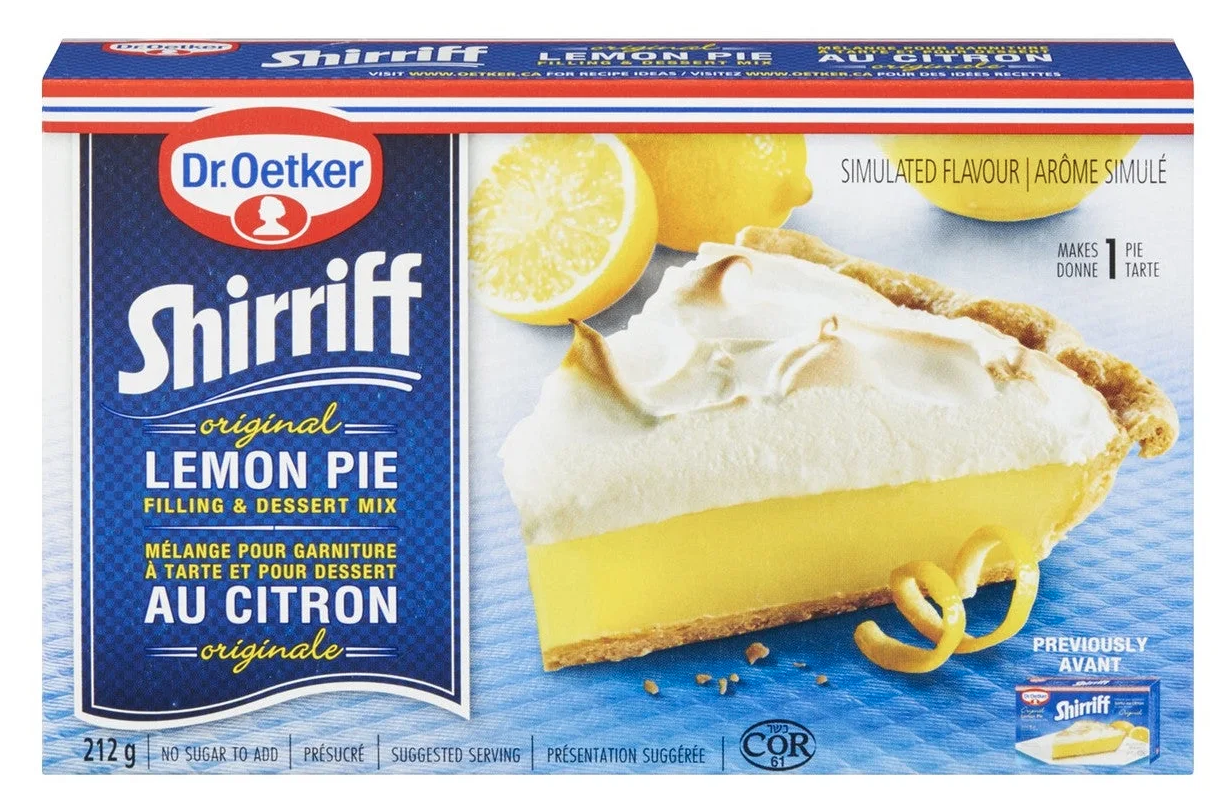
\includegraphics[width=60mm]{monanteras/images/Shirriff Lemon pie mix.png}
  \caption{Shirriff Lemon pie mix}
\end{marginfigure}

\textit{Lemon no-bake cake with peaches}

Family member: Grandma Eleni

\newthought{I have} vague memories of eating this cake during summertime on my grandma's balcony, when it was really hot and sunny. The sourness and refreshing lemon was perfect during summertime.

\begin{enumerate}
    \item Dip Goglu cookies in the juice of the canned peaches, and line them at the bottom of a large rectangular glass Pyrex.
    \item Prepare the 3 packets of Lemon pie mix following the directions. Pour the lemon mix on top of the cookies.
    \item In a small pot, warm the peach juice. Once it is boiling, add 1 tsp cornstarch and whisk until smoothe and thickened. Pour it evenly on top of the lemon curd.
    \item Whip the Nutriwhip (or Heavy cream if using) and spread it evenly on top. Add enough to create a nice 1-2 inch layer and create waves with a spoon or small spatula. 
    \item Decorate with maraschino cherries, slivered almonds, and some peaches if desired. Keep in fridge until ready to serve.
\end{enumerate}

\begin{figure}
  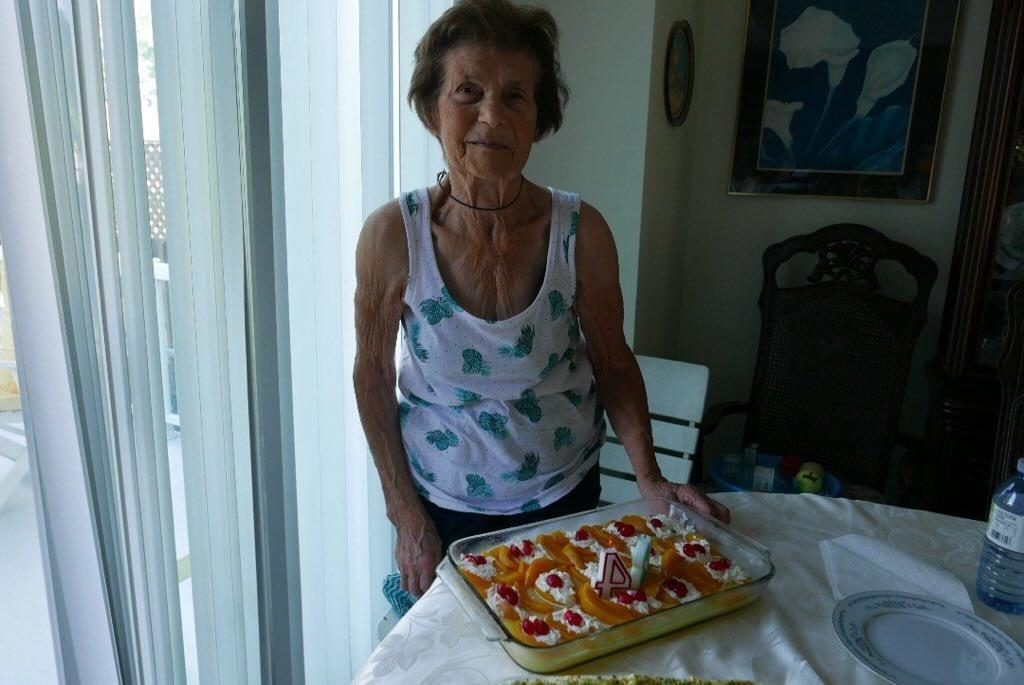
\includegraphics[width=80mm]{monanteras/images/Lemon cake.jpg}
    \caption{Celebrating Grandma's 84th birthday}
\end{figure}
\begin{figure}
  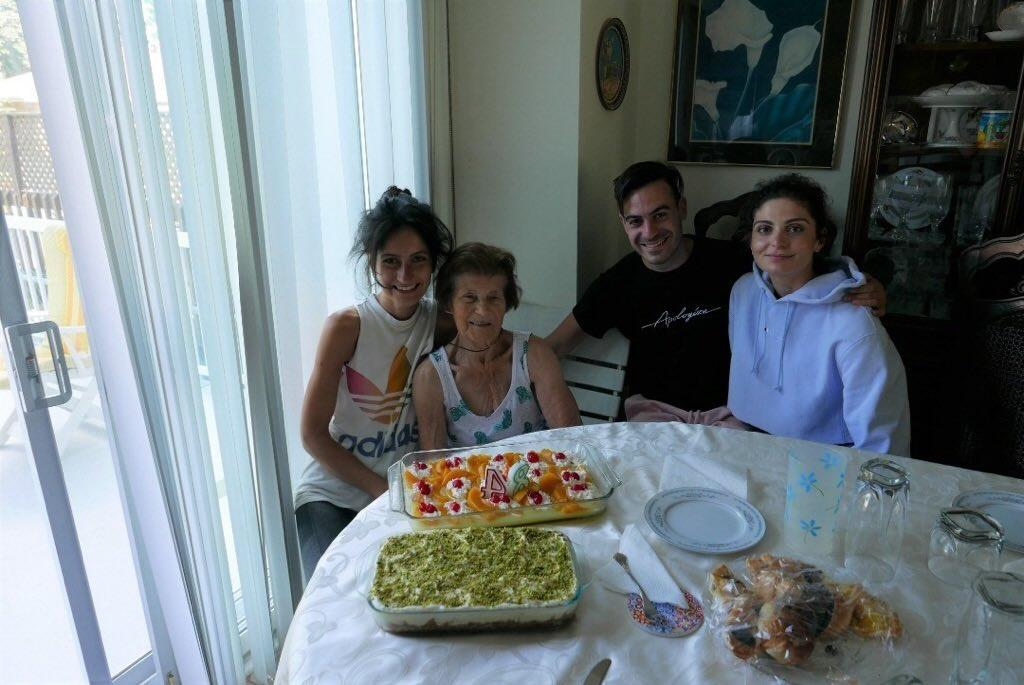
\includegraphics[width=80mm]{monanteras/images/Lemon cake 2.jpg}
\end{figure}

\chapter{Tsoureki}
\label{ch:tsoureki}
\index{dessert}
\index{bread}
\index{mahleb}
\index{Easter}

\marginnote{
    \textbf{Makes ? round braids} \\
    Prep time: 6+ hours \\
    Cook time: 30-45~minutes \\
    \vspace*{\baselineskip}

    \textbf{Ingredients for dough} \\
    11~cups all purpose flour, Five Roses \\
    1½~cups sugar \\
    1½~cups milk \\
    1½~cups butter, melted and cooled \\
    8~eggs \\
    1~tsp mahleb \\
    ½~tsp salt \\
    2~packets active yeast \\
    \vspace*{\baselineskip}

    \textbf{Ingredients to bake} \\
    Aluminium foil \\
    Colored Easter eggs \\
    2~eggs, for egg wash \\
    Slivered almonds
}

\textit{Easter bread}

Family member: Grandma Eleni

\newthought{Easter} is not Easter without \textgreek{τσουρέκι}! I can just think of the delicious smell as they're baking in the oven. If you would like to add a red Easter Egg, you can do so while shaping and bake it in the oven. Grandma \textgreek{Ελένη} would crumple a piece of foil and place it in the center of the circle to hold the shape while it bakes. Once cooled, she would remove the foil and replace it with a Easter Egg.

\begin{enumerate}
    \item In a small bowl, put the yeast with a little bit of sugar and warm water. Mix and leave it for half an hour.
    \item After half an hour, mix all the ingredients for the dough in a large bowl and leave it uncovered for 1~hour.
    \item Once 1~hour has passed, shape in braids and let them rise uncovered for 6~hours.
    \item Shape pieces of foil into small cylinders and place in the middle of each bun, where the painted eggs will go. Brush with egg wash and decorated with slivered almonds.
    \item Bake at 350-400\degree F until the tops have a golden colour and tsourekia are baked.
    \item Let cool for a few hours. Remove the foil and replace with coloured Easter eggs.
\end{enumerate}

\captionfigure{monanteras/images/Grandma eleni.JPG}{Grandma Eleni}{fig:tsoureki}

\chapter{Bikini Ladies}
\label{ch:bikiniladies}
\index{dessert}
\index{cookies}
\index{molasses}
\index{Christmas}
\textit{Gingerbread Cookies}

Family member: Elsa \& Helen

\marginnote[20pt]{\\
    \textbf{Makes 24 cookies} \\
    Prep time: 2+ hours \\
    Cook time: 7-10 minutes \\
    \vspace*{\baselineskip}

    \textbf{Ingredients for cookies} \\
    227g butter, room temperature \\
    1 cup brown sugar \\
    1/4 cup molasses \\
    1 egg \\
    2 3/4 cups all-purpose flour \\
    2 tsp cinnamon \\
    1/2 tsp cloves \\
    1 tbsp ginger \\
    2 tsp baking powder \\
    Pinch salt \\
    \vspace*{\baselineskip}
    
    \textbf{Ingredients for royal icing} \\
    2 egg whites \\
    2 tsp lemon juice \\
    3 cups icing sugar, sifted \\
}
\begin{marginfigure}[20pt]
  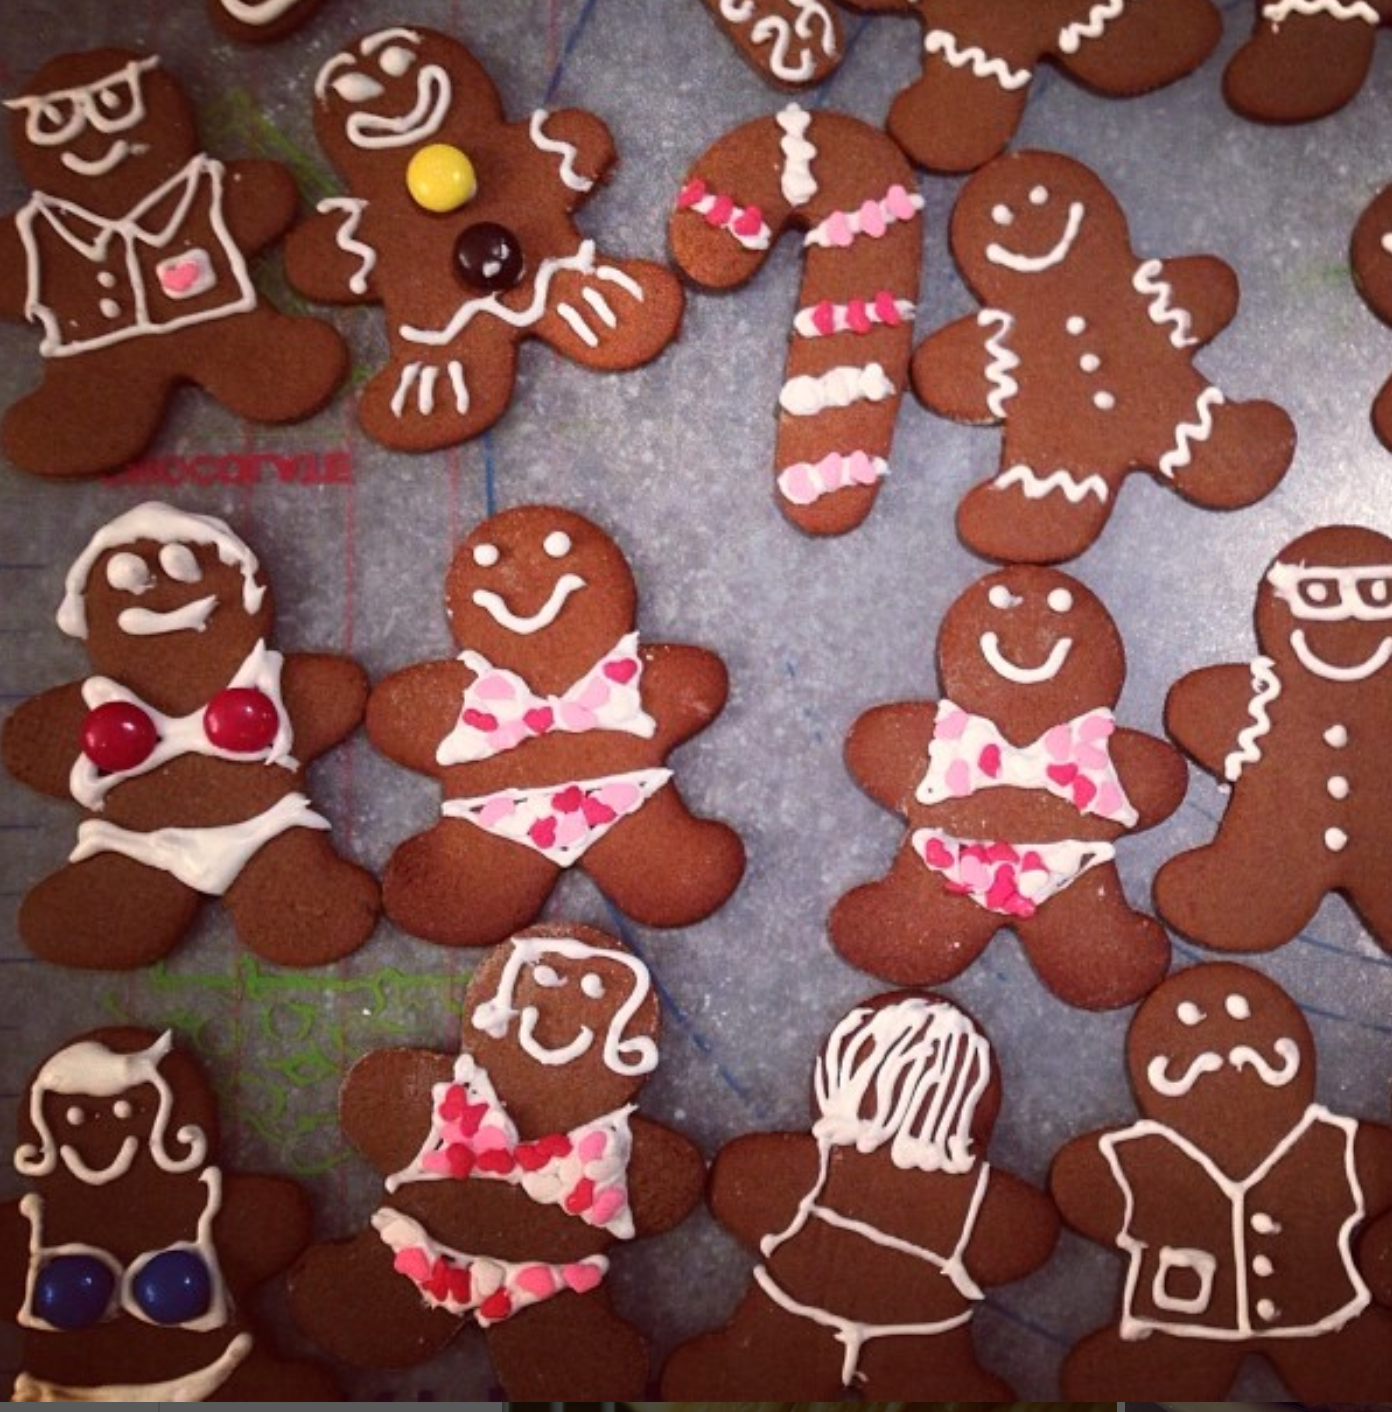
\includegraphics[width=60mm]{monanteras/images/Bikini ladies.png}
  \caption{Bikini Ladies and Hipsters}
  \label{fig:fig}
\end{marginfigure}[20pt]

\newthought{Bikini Ladies} were created because we were dreaming of the beach while we were making gingerbread cookies during winter in Montreal!

\begin{enumerate}
    \item Using a mixer, cream the butter, brown sugar and molasses until pale and fluffy. Add egg and beat until well mixed.
    \item In a large bowl, whisk the flour, spices, baking powder and salt. 
    \item Gradually add the dry ingredients to the wet, scraping down the sides of the bowl. 
    \item Shape the dough into 2 rectangles, wrap in Saran Wrap and refrigerate for 1-2 hours. Meanwhile, make royal icing following the instructions below.
    \item Once the dough is cold, flour the counter and roll it out. Keep the other dough in the refrigerator. Cut into desired shapes using Christmassy cookie cutters and place onto a baking sheet lined with parchment paper. 
    \item Chill for 30 minutes, then bake at 350\degree F for 10-12 minutes, turning midway.
    \item To make the royal icing, whisk the egg whites with lemon juice in a mixing bowl. Add the sifted icing sugar in 1 time and whisk until all is incorporated, stopping the mixer once to scrape down the sides of the bowl. If the icing is too runny, add a little more sifted icing sugar. 
    \item Cover the bowl with a damp towel to avoid a crust forming and drying out of the icing while you cook the cookies.
    \item Once the cookies have cooled down, decorate the Bikini Ladies using icing, sprinkles, candies and M \& Ms.
\end{enumerate}

\part{Elsa \& Vasken}
\chapter{Gigantes Plaki}
\label{ch:gigantes-plaki}
\index{salad}
\index{tomato}
\index{beans}

\marginnote{
    \textbf{Makes 6-8~servings} \\
    Prep time: 20~minutes \\
    Cook time: 2~hours + overnight soaking \\
    \vspace*{\baselineskip}

    500~g gigantes (lima) beans, dried and soaked in cold water overnight \\
    1~medium onion, finely chopped \\
    4-5~tbsp parsley, chopped \\
    ½~tsp celery, finely chopped \\
    1~garlic clove, minced \\
    ½~cup olive oil \\
    ¼~cup hot water + ¼~cup more if needed \\
    400~g can diced tomatoes \\
    Pinch dried oregano \\
    Salt \& pepper to taste
}

\textit{Lima beans in tomato sauce}

Family member: Elsa \& Vaski

\marginalfigure{velsa/images/Gigantes.jpg}{Gigantes}{fig:gigantes-plaki}

\newthought{Who doesn't love} a bowl of gigantes plaki with a hearty sourdough bread and a generous slice of feta?

\bigskip

\begin{enumerate}
    \item Soak the gigantes beans in cold water overnight.
    \item The next day, drain the water.
    \item On the stove, heat olive oil in a large pot (or Creuset). Add the onion and cook until translucent. Add garlic and cook 1~minute more.
    \item Add the gigantes beans and hot water. Cook for about 30~minutes on the stove top.
    \item Add the diced tomatoes, parsley, celery (if using), oregano, salt and pepper. Place in the oven at 350\degree F.
    \item Simmer until reduced and thickened, and can add the ¼~cup extra water to get wanted consistency.
    \item After about 1~hour, check peas for doneness, remove from oven and let cool.
    \item Top with more fresh parsley, serve with toasted village bread and feta.
\end{enumerate}

Do not over-stir the beans while cooking or will become mushy.
Reminds me of Fassolada or Vaski's mom's beans.

\chapter{Roasted Beet Salad with Ricotta}
\label{ch:roasted-beet-salad}
\index{salad}
\index{beet}
\index{ricotta}

\marginnote{
    \textbf{Makes 4-6~servings} \\
    Prep time: 20~minutes \\
    Cook time: 45~minutes \\
    \vspace*{\baselineskip}

    1~kg red and yellow beets, peeled and sliced \\
    1~grapefruit and 1~orange, cut into supremes and keep 1~tbsp juice of each \\
    2~tsp lemon juice \\
    1~small shallot, minced \\
    1~tbsp honey \\
    2~tbsp parsley, chopped \\
    75~g-100~g ricotta, or goat cheese \\
    55~g pistachios, toasted and chopped \\
    Olive oil \\
    Rosemary, fresh \\
    Salt \& pepper to taste
}

Family member: Elsa \& Vaski

\begin{enumerate}
    \item In a large bowl, toss beets with olive oil, rosemary, salt and pepper. If using yellow and red beets, toss separately. Place in aluminum foil pouches, onto a baking sheet and roast about 45~minutes at 400\degree F, or until you can easily poked them with a knife. Cool.
    \item Make vinaigrette: Take ½~the pistachios and grind into a coarse powder using the mortar and pestle. In a small bowl, combine the ground pistachios with the orange and grapefruit juices, lemon juice, shallot, honey, parsley and about 3~tbsp of olive oil. Whisk until well combined. Place the different coloured beets in 2~different bowls and toss them each with the vinaigrette. Season with salt and pepper.
    \item On a pretty plate, spread some of the ricotta or goat cheese and place the beets in the middle. Place the supremes of citrus and drizzle some of the vinaigrette. Add chopped parsley, chopped pistachios and some dollops of ricotta and goat cheese.
\end{enumerate}

Can keep in the fridge for a little while before serving.
Really good next to a grilled meat or lamb dish with potatoes.

\chapter{Kourabie}
\label{ch:kourabie}
\index{dessert}
\index{cookies}
\index{Christmas}

\marginnote{
    \textbf{Makes 25-30 cookies} \\
    Prep time: 45 minutes \\
    Cook time: 15-20 minutes \\
    \vspace*{\baselineskip}

    400g all-purpose flour \\
    250g butter, cold and cut into small cubes \\
    200g almonds, blanched whole \\
    1 tbsp baking powder \\
    75g icing sugar, sifted \\
    1 tbsp rosewater \\
    1/2 tsp vanilla extract \\
    1 pinch salt \\
    Icing sugar for powdering
}

\begin{marginfigure}
  \includegraphics[width=60mm]{velsa/images/Kourabie.jpg}
\end{marginfigure}

\textit{Shortbread cookies with powdered sugar and almonds}

Family member: Elsa \& Vaski

\begin{enumerate}
    \item Preheat oven to 400\degree F and toast 150g of the almonds for 7-8 minutes. Once completely cooled, pulse in a food processor until coarsely chopped and pieces remain so the cookies will be crunchy. Place them aside in a small bowl.
    \item In a food processor, add 50g of the raw almonds and blend until powdered. Set aside in another bowl.
    \item In the food processor, add the cold butter and powdered sugar. Mix for 10-15 seconds until the butter is reduced in size, almost the size of peas. Add the 50g raw powdered almonds, a pinch of salt, the rosewater and vanilla. Mix for 10-20 seconds to combine and scrape the sides. Add the baking powder and flour and mix again for 10-15 seconds.
    \item Place the mixture in a larger bowl, add the 150g toasted  chopped almonds and mix lightly with your hands.
    \item Preheat oven to 350\degree F and layer 2 baking sheets with parchment paper.
    \item Roll dough into 1 tbsp (30g) balls and place them on the baking sheets. Slightly put with your finger in the middle, to form a little dimple. Place in the fridge for 10-15 minutes before baking.
    \item Bake for 15-20 minutes until the cookies are faintly golden on the top and colored on the bottom. Be careful not to overbake them.
    \item Let them completely cool before dusting them with powdered sugar.
\end{enumerate}

\chapter{The Hybrid: Cheureg/Tsoureki}
\label{ch:cheureg}
\index{dessert}
\index{bread}
\index{mahleb}
\index{Easter}

\marginnote{
    \textbf{Makes 6 medium braids} \\
    Prep time: 5-6 hours \\
    Cook time: 30-45 minutes \\
    \vspace*{\baselineskip}

    \textbf{Dry ingredients} \\
    2-1/4 tsp instant yeast \\
    2 tsp mahleb \\
    2.5 g mastiha, freshly ground \\
    830 g AP flour, Robin Hood \\
    267 g sugar \\
    1/2 tsp salt \\
    \vspace*{\baselineskip}

    \textbf{Wet ingredients} \\
    84 g water, room T \\
    334 g whole milk, room T \\
    4 eggs, room T \\

    227 g unsalted butter, room T, very soft and cut into cubes \\
    \vspace*{\baselineskip}

    \textbf{Before baking} \\
    2 egg yolks and 1 egg white, for egg wash \\
    Slivered almonds
}

\textit{Easter bread}

Family member: Elsa \& Vaski

\newthought{Our recipe} is based on Vaski's Family Choreg recipe with a few modifications! It contains both mahleb and \textgreek{μαστίχα}. Make sure to use All purpose flour not bread flour, yields a more fluffy \mbox{Cheureg/Tsoureki}.

\begin{enumerate}
    \item In a mixing bowl, whisk the dry ingredients. In another bowl, whisk wet ingredients together. Gradually add wet ingredients to dry ingredients while mixing. Mix for 5 minutes with the paddle. Let rest for a few minutes.
    \item Mix for 5-7 minutes while adding about 90g additional flour until dough comes together and sides start to unstick. Switch to hook attachment. (If dough already has come together don't add any additional flour).
    \item Add 1/3 of the butter and mix until fully incorporated before adding another third. Do the same for the last third of the butter.
    \item Mix on medium until dough is smooth, has unstuck from the sides of the bowl and passes the windowpane test. Approximately 20 minutes of mixing total. Place dough in a bowl, cover with plastic wrap and let rise for 90 minutes in a warm place - in the oven with lights on/oven off works well!
    \item Divide dough into 80g and shape into balls. Shape into small logs and into 6 braids. If you have extra strands you can make individual kaiser buns. Let rise 1 hour to 1 hour and a half.
    \item Meanwhile, preheat the oven to 350\degree F.
    \item Brush with egg wash and add slivered almonds on top of each braid. Bake for 20 minutes, rotate pans and place another plan under pans (double) and bake for another 7 to 10+ minutes or until brown. Larger braids can be baked for 35 minutes.
    \item Cool, share with family/friends and enjoy with coffee!
\end{enumerate}

\twosidecaptionfigure{velsa/images/PXL_20240331_211621965.PORTRAIT.ORIGINAL.jpg}{velsa/images/PXL_20240331_230346663.PORTRAIT.ORIGINAL.jpg}{Tsoureki/Cheureg hybrid pre and post baking}{fig:cheureg}

\captionfigure{velsa/images/Tsoureki braid_Aki.PNG}{Four-braid braiding instructions}{fig:cheureg_braid}

% \chapter{The Best Chocolate Babka Ever}
\label{ch:babka}
\index{dessert}
\index{bread}
\index{chocolate}

\marginnote{
    \textbf{Makes 2 medium loaves or 1 giant loaf} \\
    Prep time:  hours \\
    Cook time:  minutes \\
    \vspace*{\baselineskip}

    2 ¼ tsp instant yeast \\
    2 tsp mahleb
}

\marginalfigure{velsa/images/Babka.png}{Babka}{fig:babka}

Family member: Elsa \& Vaski

\begin{enumerate}
    \item In a mixing bowl, whisk the dry ingredients. In another bowl, whisk wet ingredients together. Gradually add wet ingredients to dry ingredients while mixing. Mix for 5 minutes with the paddle. Let rest for a few minutes.
\end{enumerate}

\twosidecaptionfigure{velsa/images/PXL_20230513_194822519.jpg}{velsa/images/Babka at picnic.jpg}{Babka}{fig:babka2}

% % picture with Vaski
% {velsa/images/PXL_20230513_193701113.jpg}

% \chapter{Chocolate Chip Cookies}
\label{ch:extra-choco-chip-cookies}
\index{dessert}
\index{cookies}
\index{dessert!cookies}  % sub-category
\index{chocolate}


\marginnote[20pt]{\\
    \textbf{Makes 12 cookies} \\ \vspace*{\baselineskip}
    
    8 tablespoons of salted butter \\
    1/2 cup white sugar (I like to use raw cane sugar with a coarser texture) \\
    1/4 cup packed light brown sugar \\
    1 teaspoon vanilla \\
    1 egg \\
    1 1/2 cups all purpose flour (6.75 ounces) \\
    1/2 teaspoon baking soda \\
    1/4 teaspoon salt (but I always add a little extra) \\
    3/4 cup chocolate chips (I use a combination of chocolate chips and chocolate chunks)
}

\begin{figure}
  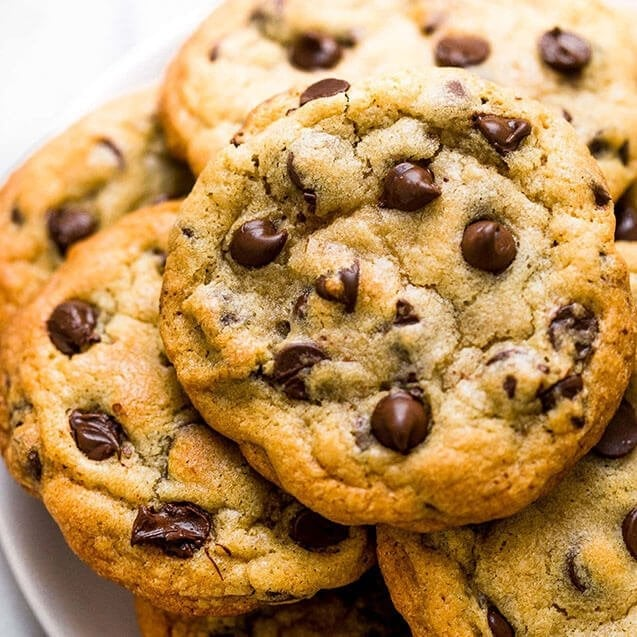
\includegraphics[width=44mm]{extra/images/BAKERY-STYLE-CHOCOLATE-CHIP-COOKIES-9-637x637-1.jpg}
  \caption{This is a cookie}
  \label{fig:marginfig}
\end{figure}


\newthought{These are the best} soft chocolate chip cookies! No chilling required. Just ultra thick, soft, classic chocolate chip cookies!

These cookies remind me of countless afternoons spent in my grandma's warm kitchen, the scent of vanilla and chocolate filling the air as we whipped up batches of these delightful treats. I can still picture her hands expertly mixing the dough, each ingredient added with care and precision. Together, we would scoop out heaping tablespoons of dough onto the baking sheets, eagerly anticipating the moment when we could sink our teeth into the warm, gooey cookies fresh from the oven.

\section{Cute}

My grandma's secret to the perfect chocolate chip cookies was simple: she never chilled the dough. Instead, she relied on a careful balance of ingredients to achieve cookies that were ultra thick, soft, and packed with chocolatey goodness. As they baked, the cookies would spread just enough to create a delicate crispness around the edges, while remaining wonderfully soft and chewy in the center.
My grandma's secret to the perfect chocolate chip cookies was simple: she never chilled the dough. Instead, she relied on a careful balance of ingredients to achieve cookies that were ultra thick, soft, and packed with chocolatey goodness. As they baked, the cookies would spread just enough to create a delicate crispness around the edges, while remaining wonderfully soft and chewy in the center.

\paragraph{Eat me!}

With each bite, memories of laughter and love flooded back, reminding me of the special bond I shared with my grandma in her kitchen. Though she may no longer be with us, her legacy lives on in every batch of these classic chocolate chip cookies, bringing comfort and joy to all who are lucky enough to enjoy them.

\bigskip

\begin{enumerate}
    \item Preheat the oven to 350 degrees. Microwave the butter for about 40 seconds to just barely melt it. It shouldn’t be hot – but it should be almost entirely in liquid form.

    \item Using a stand mixer or electric beaters, beat the butter with the sugars until creamy. Add the vanilla and the egg; beat on low speed until just incorporated – 10-15 seconds or so (if you beat the egg for too long, the cookies will be stiff).

    \item Add the flour, baking soda, and salt. Mix until crumbles form. Use your hands to press the crumbles together into a dough. It should form one large ball that is easy to handle (right at the stage between “wet” dough and “dry” dough). Add the chocolate chips and incorporate with your hands.

    \item Roll the dough into 12 large balls (or 9 for HUGELY awesome cookies) and place on a cookie sheet. Bake for 9-11 minutes until the cookies look puffy and dry and just barely golden. Warning, friends: DO NOT OVERBAKE. This advice is probably written on every cookie recipe everywhere, but this is essential for keeping the cookies soft. Take them out even if they look like they’re not done yet (see picture in the post). They’ll be pale and puffy.

    \item Let them cool on the pan for a good 30 minutes or so (I mean, okay, eat four or five but then let the rest of them cool). They will sink down and turn into these dense, buttery, soft cookies that are the best in all the land. These should stay soft for many days if kept in an airtight container. I also like to freeze them.
\end{enumerate}


%%
% The back matter contains appendices, bibliographies, indices, glossaries, etc.

\backmatter

% \bibliography{sample-handout}
% \bibliographystyle{plainnat}

\printindex

\end{document}
